% Filename map3d.tex
% Author: Rob MacLeod
%
% Last update: Sun Sep 24 16:41:08 2000 by Rob MacLeod
%    - Version 5.0Beta release edition
% Last update: Mon Jul 23 13:28:30 2001 by Rob MacLeod
%    - release 5.2
% Last update: Fri Mar 1 20:00:00 2002 by Bryan Worthen
%    - release 5.3
% Last update: Sun Feb  2 01:26:43 2003 by Rob MacLeod
%    - release 5.4
% Last update: Tue Mar 29 01:26:43 2004 by Bryan Worthen
%    - release 6.0
% Last update: Wed Jun 30 13:28:30 2004 by Bryan Worthen
%    - release 6.1
% Last update: Thu May 19 11:27:04 2005 by Rob Macleod
%    - release 6.3
% Last update: Fri Aug 26 11:27:04 2005 by Bryan Worthen
%    - release 6.4
% Last update: Fri Feb 16 08:15:11 2007 by Rob Macleod
%    - release 6.5
%%%%%%%%%%%%%%%%%%%%%%%%%%%%%%%%%%%%%%%%%%%%%%%%%%%%%%%%%%%%%%%%%%%%%
\documentclass[11pt]{article}
\usepackage{graphicx}
\usepackage{fancyhdr}
\usepackage{html}
\usepackage{manual-map3d}
\usepackage[superscript]{cite}

%\pagestyle{fancy}
\setlength{\parskip}{\smallskipamount} 
\setcounter{tocdepth}{2}
\newcommand{\pscont}{{\em pscont\/}}
\newcommand{\map}{{\em map3d\/}}
\newcommand{\mapgl}{{\em map3dGL\/}}
\newcommand{\graphicsio}{\emph{graphicsio}}
\newcommand{\eg}{{\em e.g.,}}
\newcommand{\ie}{{\em i.e.,}}
\newcommand{\etc}{{\em etc,}}
\newcommand{\splitline}{\begin{center}\rule{13cm}{.7mm}\end{center}}
\renewcommand{\topfraction}{1.0}
\renewcommand{\bottomfraction}{1.0}
\renewcommand{\textfraction}{.0}
\newcommand{\rob}{Rob MacLeod (macleod@cvrti.utah.edu)}
\newcommand{\file}[1]{\texttt{#1}}
\newcommand{\var}[1]{\texttt{#1}}
% Make sure to change this command with each new version!!
\newcommand{\version}{6.5}
\sloppy
%%%%%%%%%%%%%%%%%%%%%%%%%%%%%%%%%%%%%%%%%%%%%%%%%%%%%%%%%%%%%%%%%%%%%
\begin{document}

\thispagestyle{empty}
% -*-latex-*-
% Document name: title.tex
% Creator: Rob MacLeod [macleod@vissgi.cvrti.utah.edu]
% Last update: September 2, 2000 by Rob MacLeod
%    - created
% Last update: Sun Sep 24 16:41:08 2000 by Rob MacLeod
%    - Version 5.0Beta release edition
% Last update: Mon Jul 23 13:28:30 2001 by Rob MacLeod
%    - release 5.2
% Last update: Fri Mar 1 20:00:00 2002 by Bryan Worthen
%    - release 5.3
% Last update: Fri Jan 24 20:00:00 2003 by Bryan Worthen
%    - release 5.4
% Last update: Tue Mar 30 20:00:00 2003 by Bryan Worthen
%    - release 6.0
% Last update: Wed Jun 30 20:00:00 2003 by Bryan Worthen
%    - release 6.1
% Last update: Wed Oct 18 20:00:00 2003 by Bryan Worthen
%    - release 6.2
% Last update: Thu May 19 11:27:26 2005 by Rob Macleod
%    - version 6.3
% Last update: Fri Aug 26 11:27:26 2005 by Bryan Worthen
%    - version 6.4
%%%%%%%%%%%%%%%%%%%%%%%%%%%%%%%%%%%%%%%%%%%%%%%%%%%%%%%%%%%%%%%%%%%%%%
  \mbox{}
  \vspace{2in}
\begin{center}
   {\huge\bf \map{} User's Guide}\\
   \vspace{.5in}
   {\Large Version \version{}\\
   \medskip
   Last update: Aug 26, 2005 \\}
   \bigskip
   {\Large Authors: \rob{}, \\
   Bryan Worthen (worthen@sci.utah.edu), and \\
   J.R. Blackham (blackham@sci.utah.edu)}
   \bigskip

   {\Large 
   \medskip
   Scientific and Computing Institute (SCI)\\
   \htmladdnormallink{www.sci.utah.edu}
   {http://www.sci.utah.edu/}\\
   \medskip
   Center for Bioelectric Field Modeling, Simulation and Visualization
   \htmladdnormallink{www.sci.utah.edu/ncrr}{http://www.sci.utah.edu/ncrr}\\
   \medskip
   Nora Eccles Harrison \\
   Cardiovascular Research and Training Institute (CVRTI)\\
%   \smallskip
   \htmladdnormallink{www.cvrti.utah.edu}
   {http://www.cvrti.utah.edu/}\\
   \medskip
   the University of Utah}\\

   \bigskip
   Support for this project came from:\\
   \medskip
   {\Large The NIH National Center for Research Resources  
   \htmladdnormallink{(NCRR)}{http://www.ncrr.nih.gov} and the The Nora
   Eccles Treadwell Foundation\\ 
   \smallskip
   }

\end{center}

%%% Local Variables: 
%%% mode: latex
%%% TeX-master: "manual"
%%% End: 

\newpage

\tableofcontents
\splitline

\newpage

%%%%%%%%%%%%%%%%%%%%%%%%%%%%%%%%%%%%%%%%%%%%%%%%%%%%%%%%%%%%%%%%%%%%
 % -*-latex-*-
% Document name: newfeatures.tex
% Creator: Rob MacLeod [macleod@vissgi.cvrti.utah.edu]
% Last update: September 2, 2000 by Rob MacLeod
%    - created
% Last update: Mon Jul 23 13:28:30 2001 by Rob MacLeod
%    - release 5.2
% Last update: Fri Mar 1 20:00:00 2002 by Bryan Worthen
%    - release 5.3
% Last update: Fri Jan 24 20:00:00 2003 by Bryan Worthen
%    - release 5.4
% Last update: Tue Mar 30 20:00:00 2004 by Bryan Worthen
%    - release 6.0
% Last update: Wed Jun 30 13:28:30 2004 by Bryan Worthen
%    - release 6.1
% Last update: Tue Oct 19 13:28:30 2004 by Bryan Worthen
%    - release 6.2
% Last update: Wed May 11 13:28:30 2005 by Bryan Worthen
%    - release 6.3
% Last update: Thu May 19 12:35:15 2005 by Rob Macleod
%    - for version 6.3
% Last update: Fri Aug 26 12:35:15 2005 by Bryan Worthen
%    - for version 6.4
%%%%%%%%%%%%%%%%%%%%%%%%%%%%%%%%%%%%%%%%%%%%%%%%%%%%%%%%%%%%%%%%%%%%%%
%%%%%%%%%%%%%%%%%%%%%%%%%%%%%%%%%%%%%%%%%%%%%%%%%%%%%%%%%%%%%%%%%%%%
\section{What's New?}
\label{sec:new-features} 

In this section, we highlight the latest additions to \map{} in the
(vain?) hope that people will read at least this much of the manual
and be able to quickly make use of the latest and greatest that the program
offers.

\subsection{Version~\version{}: Aug, 2005}

This is the fifth version of the ``new'' \map{} with a GTK-based GUI.  We
are getting much closer to the complete functionality of the old GL
based version and have gone well beyond it in some features, especially the
user interface.  This is a ``dot'' release, and this release contains
a number of bug fixes and GUI enhancements.

Some of the specific additions that you should notice over previous versions
include:
%
\begin{description}
  \item [GUI improvements: ] Some improvements in the GUIs, particularly in the
    fiducial control and contour spacing control.  See 
    Section~\ref{sec:interactive}.
  \item [Saving Matlab Geometry: ] This version allows the user to save matlab 
    geometry files, single or multiple surfaces per file.
  \item [Bug fixes: ] not that the previous version had any bugs, but we
    found a few(!) things to fix.
\end{description}

\subsection{In the works (``vapourware'')}
\label{sec:vapourware}

A small sampler of things that are in the works:

\begin{itemize}
  \item Incorporating fiducials into the matlab format
  \item Saving the frames into actual movies.
  \item Dynamic menus that indicate the current parameter selections
    (a bit more in progress).
  \item New display modes for the display of vectors.
  \item Fixing the bugs listed on the bugs page (see
    Section~\ref{sec:bugs}).
\end{itemize}



%%% Local Variables: 
%%% mode: latex
%%% TeX-master: "manual"
%%% End: 

\newpage
% -*-latex-*-
% Document name: intro.tex
% Creator: Rob MacLeod [macleod@vissgi.cvrti.utah.edu]
% Last update: September 2, 2000 by Rob MacLeod
%    - created
% Last update: Sun Sep 24 16:41:08 2000 by Rob MacLeod
%    - Version 5.0Beta release edition
% Last update: Mon Jul 23 13:28:30 2001 by Rob MacLeod
%    - release 5.2
% Last update: Fri Mar 1 20:00:00 2002 by Bryan Worthen
%    - release 5.3
% Last update: Sun Feb  2 01:54:43 2003 by Rob MacLeod
%    - Release 5.4
% Last update: Thu May 19 12:35:15 2005 by Rob Macleod
%    - for version 6.3
% Last update: Fri Feb 16 08:24:13 2007 by Rob Macleod
%    - verison 6.5
% Last update: Fri Jul 22 16 22:15:11 2016 by Bryan Worthen
%    - release 7.2.2
%%%%%%%%%%%%%%%%%%%%%%%%%%%%%%%%%%%%%%%%%%%%%%%%%%%%%%%%%%%%%%%%%%%%%%
\section{Introduction}

This document describes the function and usage of version~\version{} of the
program \map{}, a scientific visualization application originally developed
at the Nora Eccles Harrison Cardiovascular Research and Training
\htmladdnormallink{(CVRTI)}{http://www.cvrti.utah.edu} and now under
continued development and maintenance at the Center for Integrative
Biomedical Computing (CIBC), which is an NIH/NCRR funded center hosted by
the Scientific Computing and Imaging Institute
\htmladdnormallink{(SCI)}{http://www.sci.utah.edu} at the University of
Utah.  The original purpose of the program was to interactively view scalar
fields of electric potentials from measurements and simulations in cardiac
electrophysiology.  Its present utility is much broader but continues to
focus on viewing three-dimensional distributions of scalar values
associated with an underlying geometry consisting of node points joined
into surface or volume meshes.

\map{} has been the topic of some papers
\cite{RSM:Mac92c,RSM:Mac92d,RSM:Mac93,RSM:Mac93a} and a technical report
\cite{RSM:Mac94d} and we'd love it if you would reference at least one of
them (perhaps \cite{RSM:Mac93} or \cite{RSM:Mac93a} are the easiest ones to
get copies of) as well as this manual when you publish results using it.
There have been many many more papers that use \map{} and the list keeps
growing.\cite{RSM:Mac93,RSM:Mac93a,RSM:Mac94d,RSM:Mac94c,RSM:Mac94f,RSM:Mac95d,RSM:Mac97,RSM:Mac98,RSM:Mac2000a,RSM:Mac2001,RSM:Pun98,RSM:Pun99,RSM:Tac92,RSM:Tac92b,RSM:Tac94,RSM:Tac96,RSM:Tac96b,RSM:Tac97b,RSM:Ni98,RSM:Ni99,RSM:Ni2000b,RSM:Lux96,RSM:Lux2001,CRJ:Joh93b,CRJ:Joh93d,CRJ:Joh94,CRJ:Joh94b,RSM:Pun2003,RSM:Ser2002}

As with our past versions, this edition of \map{} is completely open
source.  Anyone can download not only the executable for some major
platforms (OSX, Windoze) but also the complete source code for
the program.  Please note that we do not have a good way yet to incorporate
changes people outside our little group make to the program.  If you do
wish to change and then contribute back, please let us know as soon as
possible and we can try and coordinate as best we can.  Of special interest
are any ports of \map{} to another platform---please let us know about this
and we can add it to the list and release it with the rest.

\subsection{Acknowledgments}

The history of \map{} goes back to 1990 and the first few hundred lines of
code were the product of a few hours work by Mike Matheson, an inspired
visualization specialist, now with SGI in Salt Lake City.  This was my
(Rob) introduction to GL and C and this program became my personal sand box
to play in.  Along the way, Phil Ershler made valuable contributions in
figuring out the magic of Formslib for some user interface controls and
developing with me \emph{graphicsio}, the geometry and data file library
that supports \map{}.  Ted Dustman has recently taken up maintenance and
extensions of \emph{graphicsio} and remains my main man when I need
programming lessons.

This is one in a series of ``new'' versions of \map{}, the series (labeled
5.x or above) that marks the move from GL to OpenGL library and thus to
becoming truly portable.  In fact, we call the old one \mapgl{} now to
indicate its links to SGI's original GL library.  We seem permanently stuck
in the middle of this big conversion project, moving support to OpenGL and
adding lots of power as we convert functionality.  The reason for the
version 6.x, was the move to gtk as the GUI library with which we create
all the dialog and display elements of the program.  This move has allowed
us to extend dramatically the set of dialog boxes \map{} offers. 
Version 7.x moved again to the Qt toolkit, preserving the spirit of the dialogs of the Gtk+ version, and this
newest version \version{} contains many examples.

There are some people who have been instrumental in the process and deserve
special mention.  Chris Moulding is a graphics programmer and general
software whiz who surveyed my sand box architecture, pulled together the
essential walls, created new ways to make rooms, and still left lots of the
sand box around so we could continue to play.  From version 5.2 onward,
Bryan Worthen replaced Chris and really has found the spirit of \map{}.
Bryan has become the main driving force behind the actual work of coding
and fixing.  He strayed off to some other project for a while, but never
lost his love for \map{}; we are really pleased that he has returned to
pick up the torch again. J.R. Blackham joined the team in about 2003 while
finishing an undergraduate in Computer Science at Utah and a little after.
Jeroen Stinstra
is my super-postdoc, helpful in more ways than I knew I even needed and
full of inventive ideas.  He has created the support for MATLAB that we use
in \map{} (and the SCIRun project) and is best bug-catcher I know.

The largest thanks must go to the users of \map{}, who provided the real
inspiration and identified the needs and opportunities of such a program.
Among the most supportive and helpful are Bruno Taccardi, Bonnie Punske,
and Bob Lux, all colleagues of mine at the CVRTI. Dana Brooks and his
students from Northeastern University are also regular users who have
provided many suggestions and great enthusiasm.  Also invaluable in the
constant improvement of the program are my post docs, Jeroen Stinstra, and
graduate student Quan Ni, Rich Kuenzler, Bulent Yilmaz, Bruce Hopenfeld,
Shibaji Shome, Lucas Lorenzo, Andrew Shafer, and Zoar Englemann.  They give
me new energy every day and remind me why I am a professor.  Notable new
additions to the family are Randy Thomas from Universite d'Evry Val
d'Essonne in Evry, France.  The great thing about Randy is that he used
\map{} to visualize concentrations of ions in his simulation of the
nephron!  Also, Ed Ciaccio from Columbia University has become a big user
and even takes it to his classes.

The first user and long-time collaborator and friend was Chris Johnson and
this new version of \map{} is possible because of the success he and I have
had in creating the SCI Institute and specifically the NIH/NCRR Center for
Integrative Biomedical Computing (\htmladdnormallink{www.sci.utah.edu/cibc}
{www.sci.utah.edu/cibc}).

We gratefully acknowledge the financial support that has come from the NIH,
National Center for Research Resources
\htmladdnormallink{(NCRR)}{http://www.ncrr.nih.gov}, the Nora Eccles
Treadwell Foundation, and the University of Utah, which provides us with
space and materials to create this sand box.  The Nora Eccles Treadwell
Foundation has provided support not only for the development of \map{} but
also the experiments that provide the huge pile of data we have used \map{}
to analyze.

\bigskip
\noindent
Rob MacLeod, June, 2017.


\subsubsection{Open Source License}
\label{sec:source_license}

The terms of the license agreement under which we release \map{} are simple
and as follows:

\begin{quotation}

Permission is hereby granted, free of charge, to any person obtaining a
copy of this software and associated documentation files (the
``Software''), to deal in the Software without restriction, including
without limitation the rights to use, copy, modify, merge, publish,
distribute, sublicense, and/or sell copies of the Software, and to permit
persons to whom the Software is furnished to do so, subject to the
following conditions:
\begin{enumerate}
  \item The above copyright notice and this permission notice shall be
    included in all copies or substantial portions of the Software.
  \item Use of this software in preparing any publication material must be
    cited as follows:
    
    \vspace{0.1in}
    
    R.S. MacLeod and C.R. Johnson. Map3d: Interactive scientific
    visualization for bioengineering data. In IEEE Engineering in
    Medicine and Biology Society 15th Annual International Conference,
    pages 30-31, IEEE Press, 1993.
\end{enumerate}
\vspace{0.1in}

THE SOFTWARE IS PROVIDED ``AS IS'', WITHOUT WARRANTY OF ANY KIND, EXPRESS
OR IMPLIED, INCLUDING BUT NOT LIMITED TO THE WARRANTIES OF MERCHANTABILITY,
FITNESS FOR A PARTICULAR PURPOSE AND NONINFRINGEMENT. IN NO EVENT SHALL THE
AUTHORS OR COPYRIGHT HOLDERS BE LIABLE FOR ANY CLAIM, DAMAGES OR OTHER
LIABILITY, WHETHER IN AN ACTION OF CONTRACT, TORT OR OTHERWISE, ARISING
FROM, OUT OF OR IN CONNECTION WITH THE SOFTWARE OR THE USE OR OTHER
DEALINGS IN THE SOFTWARE.
\end{quotation}


\subsubsection{Libraries used by \map{}}

\map{} incorporates the functionality of several external libraries.  They
are:
\begin{itemize}
  \item \htmladdnormallink{Qt}{https://www.qt.io} - Qt -
    Copyright (C) 2016 The Qt Company
  \item \htmladdnormallink{PNG}{http://www.libpng.org} - Copyright (c)
    1998-2002 Glenn Randers-Pehrson 
  \item \htmladdnormallink{Jpeglib}{http://www.ijg.org} - Copyright (C)
    1991-1998, Thomas G. Lane.
\end{itemize}

We use Qt to interface with the window manager to give us
windows with OpenGL capability, as well as giving us widgets we need for
interactive control.  We use PNG and JpegLib to be able to save
\texttt{.png} and \texttt{.jpg} images of \map{}.
All of these libraries are covered by the \htmladdnormallink{GNU
LGPL}{http://www.gnu.org/licenses/lgpl.html}, which is included in the
distribution of \map{}.

As of version~\version{}, we also release internal libraries under the
same license as above for the rest of \map{}.  

\subsection{Documentation}

This document should have reached you either as a pdf file or via the
\htmladdnormallink{\map{} web site}
{http://www.sci.utah.edu/software/map3d.html}.  If you would like more
copies or the latest version, go to the
same web site and look for the links under Documentation:\\

\htmladdnormallink{\texttt{www.sci.utah.edu/software/map3d.html}}
{http://www.sci.utah.edu/software/map3d.html}

\subsection{Bug reporting}
\label{sec:bugs}

We want to hear your response to using \map{} and especially to learn about
any bugs you may find.  They may be features, rather than bugs, but if so,
we will be happy to hear your impressions.

To submit a bug report please send email to 
\htmladdnormallink{map3d@sci.utah.edu} {mailto:map3d@sci.utah.edu}
or point your browser at
\htmladdnormallink{\map{} issue tracker}{https://github.com/SCIInstitute/map3d/issues}
(you will need to register your e-mail
address) with the following information:

\begin{enumerate}
  \item Type and version of the operating system and hardware you are using.
  \item Version of \map{}.
  \item Description of the bug/feature you encountered.
  \item Suggestions for fixing the bug or altering the program behavior.
\end{enumerate}


Here is a short list of the issues we know about and are currently addressing:

\begin{itemize}
  \item When adding surfaces or updating time series data interactively,
    there can be surprises with scaling.  The easy solution is to adjust
    the scaling in some small way and the resulting update usually takes
    care of the problem.
\end{itemize}



\subsection{How to reach us}

We have established an email address for \map{},
\htmladdnormallink{map3d@sci.utah.edu}{mailto:map3d@sci.utah.edu}, and
web pages within the website \htmladdnormallink{www.sci.utah.edu/ncrr}
{http://www.sci.utah.edu/ncrr} dedicated to \map{}.  There is also a
majordomo mailing list for \map{} users called
\texttt{map3d-users@sci.utah.edu}.  To subscribe to this list, send email to
\texttt{majordomo@sci.utah.edu} with the following in the message body\\
%
\begin{verbatim}
      subscribe map3d-users
\end{verbatim}

Please let us know how you use \map{} and how we can make it better for
your purposes.  We can only develop this program with continued
support and the best way to achieve this is to show that others use the
program and find it helpful.





%%% Local Variables: 
%%% Local Variables: 
%%% mode: latex
%%% TeX-master: "manual"
%%% TeX-master: "manual"
%%% TeX-master: "manual"
%%% End: 

\newpage
% -*-latex-*-
% Document name: install.tex
% Creator: Rob MacLeod [macleod@vissgi.cvrti.utah.edu]
% Last update: Fri Sep 15 00:33:54 2000 by Rob MacLeod
%    - created
% Last update: Wed Sep 27 14:54:43 2000 by Rob MacLeod
%    - some fixes for bug reporting and spell checking
% Last update: Sun Sep 24 16:41:08 2000 by Rob MacLeod
%    - Version 5.0Beta release edition
% Last update: Mon Jul 23 13:28:30 2001 by Rob MacLeod
%    - release 5.2
% Last update: Fri Jun 21 13:32:48 2002 by Rob Macleod
%    - release 5.3
% Last update: Fri Jan 24 20:00:00 2004 by Bryan Worthen
%    - release 5.4
% Last update: Thu May 19 12:35:15 2005 by Rob Macleod
%    - for version 6.3
% Last update: Fri Aug 26 12:34:14 2005 by Bryan Worthen
%    - for version 6.4
% Last update: Fri Feb 16 08:32:27 2007 by Rob Macleod
%    - version 6.5
%%%%%%%%%%%%%%%%%%%%%%%%%%%%%%%%%%%%%%%%%%%%%%%%%%%%%%%%%%%%%%%%%%%%%%
\section{Installation}

\subsection{System requirements}

\map{} is written in standard C/C++ and uses the OpenGL and GTK+ libraries, 
both choices made to ensure broad portability of the program.

Note: As of \map{} 6.4 or greater, GTK+ version 2.4 or greater is required
to run \map{}.  Please update your dependencies according the the 
Windows, Linux, or Mac sections below.

  \begin{description}
    \item [All platforms: ]  OpenGL now comes standard on most systems.  
          Instructions on how to install GTK+ are described in detail below
          based on which platform you are installing.
          described below\mbox{}\\
          \begin{center}
          \begin{tabular}{|l|l|} \hline
            \multicolumn{2}{|c|}{Requirements for all systems.  } \\ \hline
          OpenGL libraries (GL and GLU) & version 1.1 +
     \footnote{A plus sign, ``+'', indicates ``or better''}\\
            OpenGL/window interface library (GLX)& \\
            \htmladdnormallink{GTK+}
            {http://www.gtk.org} 
            libraries and dependencies & version 2.4+ \\ 
            gtkglext: GL extension for GTK & 1.2+ \\ \hline
            
          \end{tabular}
          \end{center}

            
    \item [Linux (i386): ] \map{} requires the OpenGL library, which is
              available 
          as the mesa library at \htmladdnormallink{www.mesa3d.org}
          {http://www.mesa3d.org} for any Linux platform.  For better
          performance, graphics cards from companies such as nVidia 
          \htmladdnormallink{(www.nvidia.com)}
          {http://www.nvidia.com/} usually provide OpenGL libraries.  \\
          \begin{center}
          \begin{tabular}{|l|l|} \hline
            \multicolumn{2}{|c|}{Requirements} \\ \hline
              Operating System & kernel 2.2.x\\
              Architecture & i386 (+ maybe PPC)\\
              Applications Binary Interface  &  libc2.1 \\
              \hline
            \multicolumn{2}{|c|}{Recommendations} \\ \hline
            Window system & XFree86 version 4.0 +\\
            Hardware & 3D graphics card (nVidia, 3dfx, ati)\\
            & $\ge$ 128 MB main memory \\ \hline
          \end{tabular}
          \end{center}
          
    \item [Windows: ] \mbox{}\\
          \begin{center}
          \begin{tabular}{|l|l|} \hline
            \multicolumn{2}{|c|}{Requirements} \\ \hline
              Operating System & W2K/NT4.0/9x\\
              Architecture & i386\\
              Applications Binary Interface  &  win32 \\
              \hline
            \multicolumn{2}{|c|}{Recommendations} \\ \hline
            Hardware & 3D graphics card (nVidia, 3dfx, ati)\\
            & $\ge$ 128 MB main memory \\ \hline
          \end{tabular}
          \end{center}

    \item [Mac OS X: ] \mbox{}\\
          \begin{center}
          \begin{tabular}{|l|l|} \hline
            \multicolumn{2}{|c|}{Requirements} \\ \hline
              Operating System & Mac OS 10.4(Tiger)\\
              Architecture & PPC or Intel\\
              \hline
            \multicolumn{2}{|c|}{Recommendations} \\ \hline
            Hardware & 3D graphics card (nVidia, 3dfx, ati)\\
            & Intel processor \\
            & $\ge$ 512 MB main memory \\ \hline
          \end{tabular}
          \end{center}
          
   \item [SGI: ] we have dropped our support for SGI.  This platform, while
     so central to the origins of \map{} and OpenGL, is just not a
     significant desktop system in this day and age.  

  \end{description}
  
\subsection{General Installation}

Unfortunately, with our move to GTK+ for window support, it is not as easy
as past versions, which required just the download of an executable.  We
hope (in vain, perhaps) to be able to do that again in the future, but for
now we will attempt to make installation as easy as we can.  Simplified
instructions will be in a README file which comes with each package, and
are also listed below:

To download the software, use this URL
\htmladdnormallink{\texttt{www.sci.utah.edu/software/map3d.html}}
{http://www.sci.utah.edu/software/map3d.html}, and click on the
``Download'' button.  You'll need to sign into the SCI archive.  For
each of the installation instructions below, you can grab those file
from this page.


To test the installation, use the test files that accompany this
distribution.  Each has some script files included that show how to call
and execute \map{}.

% -*-latex-*-
% Document name: linux_install.tex
% Creator: Bryan Worthen [worthen@sci.utah.edu]
% Last update: Wed Oct 20 20:00:00 2004 by J.R. Blackham
%    - release 6.2
%%%%%%%%%%%%%%%%%%%%%%%%%%%%%%%%%%%%%%%%%%%%%%%%%%%%%%%%%%%%%%%%%%%%%%
\subsection{Linux Installation Instructions}
\label{sec:linux-install}

The Linux installation is relatively straightforward.  You'll need to 
download \map{}'s dependencies, then download \map{} itself.

\subsubsection{Linux Dependencies}

Basically, here you need to install Qt's development distribution.The easiest way to do this is from your distribution's 
installation CDs, or you can download the RPMs at www.rpmfind.net.  

To get the dependencies from your distribution, run the Package Manager
(Add/Remove Applications, configure-packages or something of that sort).
Search for qtk, and install gtk2 (if you can't find that directly, then 
installing the gnome environment will take care of it).

To get the dependencies from the internet, navigate your favorite browser
to \htmladdnormallink{\texttt{http://www.rpmfind.net}} {http://www.rpmfind.net}, and
search for \texttt{qt}.  Try to find one that matches your
distribution (redhat, fedora, etc.). \map{} requires qt-5.4 or greater.

\subsubsection{Linux Executable}

We do not presently support Linux binaries.  Building \map() from source
is possible.  Download the \map{} source tarball file from the \map{} download page
and unzip it to a directory of your choice.

These instructions are not complete, but the gist is: Go to the \map{} directory, run qmake, and make.
The \map{} executable will be in client/release/map3d.

%%% Local Variables: 
%%% mode: latex
%%% TeX-master: "manual"
%%% End: 

% -*-latex-*-
% Document name: windows_install.tex
% Creator: Bryan Worthen [worthen@sci.utah.edu]
% Last update: Fri Mar 26 20:00:00 2004 by Bryan Worthen
%    - release 6.0
%%%%%%%%%%%%%%%%%%%%%%%%%%%%%%%%%%%%%%%%%%%%%%%%%%%%%%%%%%%%%%%%%%%%%%
\subsection{Windows Installation Instructions}
\label{sec:windows-install}

The Windows installation is relatively straightforward.  You'll need to 
download \map{}'s dependencies, then download \map{} itself.

\subsubsection{Windows Dependencies}

Download the \texttt{map3d-win-environment.zip} file from the \map{}
\htmladdnormallink{\texttt{download page}}
{http://www.sci.utah.edu/software/map3d.html} and unzip (using winzip,
native windows xp zip file browser, or another windows zip program) it into a location
of your choice - we will call that \texttt{INSTALL-DIR.}  It will create a
directory called \verb|INSTALL-DIR\map3d|.

Add \verb|INSTALL-DIR\map3d\lib| to your path.  To do this, open the
Control Panel, select System, and click on the `Advanced' tab on the top of
the screen.  Click on the Environment Variables button.  You should see a
variable called Path or PATH in the System Variables section.  Click on it,
and select Edit.  Go to the end of the line, add a semi-colon (;) and type
\verb|INSTALL-DIR\map3d\lib|.

\subsubsection{Windows Executable}

There is an executable of map3d in the environment directory.  We have also
placed an executable here to facilitate future downloads, so you only have
to download the environment once.  If you wish, download the
\texttt{map3d-6.5-windows.zip} file from the \map{} download page and unzip
it to a directory of your choice.  We will call that \texttt{RUN-DIR.} This
is the directory from which you will run \map{}.



%%% Local Variables: 
%%% mode: latex
%%% TeX-master: "manual"
%%% End: 

% -*-latex-*-
% Document name: mac_install.tex
% Creator: J.R. Blackham [blackham@sci.utah.edu]
% Last update: Fri Jun 30 15:00:00 2004 by J.R. Blackham
%    - release 6.5
%%%%%%%%%%%%%%%%%%%%%%%%%%%%%%%%%%%%%%%%%%%%%%%%%%%%%%%%%%%%%%%%%%%%%%
\subsection{Mac OS X Installation Instructions}
\label{sec:mac-install}

The Mac OS X installation is relatively straightforward.  You'll need to 
download \map{}'s dependencies, then download \map{} itself.

\subsubsection{Mac OS X Dependencies}

Map3d requires the gtk+2 and gtkglext libraries.  We provide an installer that installs these libraries with the Mac OS X distribution of map3d.  Once you mount the \texttt{map3d-6.5-mac.dmg} disc image there is an installer application called map3d Dependencies.mpkg, just run this program and the libraries will be installed for you.


\subsubsection{Mac OS X Executable}

Also in the \texttt{map3d-6.5-mac.dmg} disc image is a file called \map{}, this is the \map{} executable and to install it, just drag it to a directory of your choice.  We will call that \texttt{RUN-DIR}. This is the directory from which you will run \map{}.





%%% Local Variables: 
%%% mode: latex
%%% TeX-master: "manual"
%%% End: 

%% -*-latex-*-
% Document name: sgi_install.tex
% Creator: Bryan Worthen [worthen@sci.utah.edu]
% Last update: Fri Mar 26 20:00:00 2004 by Bryan Worthen
%    - release 6.0
%%%%%%%%%%%%%%%%%%%%%%%%%%%%%%%%%%%%%%%%%%%%%%%%%%%%%%%%%%%%%%%%%%%%%%
\subsection{SGI Installation Instructions}
\label{sec:sgi-install}

The SGI installation is relatively straightforward.  You'll need to 
download \map{}'s dependencies, then download \map{} itself.

\subsubsection{SGI Dependencies}
There are two phases to this part.  First we need to get GTK+ and its
dependencies.  The easiest way to do this is for SGI is to run a browser
with root access and go to SGI's freeware site at \htmladdnormallink
{\texttt{http://freeware.sgi.com}} {http://freeware.sgi.com}.  On that page
near the bottom there should be a link to a prereq calculator.  Click on
that link, and in the Freeware Product box, select \verb|fw_gtk2+| (make
sure you don't select \verb|fw_gtk+|).  Submit the query.  You should see a
list similar to this:
\begin{verbatim}
  fw_atk [relnotes] [prereqs] [install] 
  fw_expat [relnotes] [prereqs] [install] 
  fw_freetype2 [relnotes] [prereqs] [install] 
  fw_gettext [relnotes] [prereqs] [install] 
  fw_glib2 [relnotes] [prereqs] [install] 
  fw_libjpeg [relnotes] [prereqs] [install]
  fw_libpng [relnotes] [prereqs] [install]
  fw_libz [relnotes] [prereqs] [install]
  fw_pango [relnotes] [prereqs] [install]
  fw_tiff [relnotes] [prereqs] [install] 
\end{verbatim}
To install them, click on the install link one by one (and follow the 
instructions in the dialog boxes). 

IMPORTANT - when you install libz - it will mention something about a security
library being removed.  When you install libz, allow it to do this.  On the 
subsequent libraries, it will mention that the security package conflicts 
with libz, on these packages, have it continue without installing the
security package.

Install them in the order:

\begin{verbatim}
    gettext
    expat
    freetype2
    atk
    glib2
    pango
    libjpeg
    libtiff
    libz
    libpng
\end{verbatim}

After you've done all of these, click on the alphabetical link, and click on
the install buton that corresponds to \verb|libgtk2+-2.0.6|.

If for some reason, the prereq calculator isn't there or isn't working, go
to the alphabetical index and install the above in the order specified.


The next part is to download gtkglext, the library that supports OpenGL for
GTK widgets.  If your GTK version is 2.0.6 (you can find out by looking at
\texttt{gtkversion.h} which will be where you installed gtk (normally
\texttt{/usr/freeware/include/gtk-2.0/gtk/gtkversion.h}), and look for
\verb|GTK_MAJOR_VERSION|, \verb|GTK_MINOR_VERSION|, and
\verb|GTK_MICRO_VERSION|.  There will be numbers on the same lines as each
of these, and if you put them together it will be something like 2.0.6).
If you are using this version download \texttt{gtkglext-sgi.tar.gz} from
the \map{} download page
\htmladdnormallink{\texttt{http://www.sci.utah.edu/software/map3d.html}}
{http://www.sci.utah.edu/software/map3d.html} and follow these
instructions:

\begin{verbatim}
    cd <download directory>
    gunzip gtkglext-sgi.tar.gz
    tar xf gtkglext-sgi.tar
    cp libgtkglext-x11-1.0.so.0 /usr/local/lib
    cp libgdkglext-x11-1.0.so.0 /usr/local/lib
\end{verbatim}

You can copy them to some directory other than \texttt{/usr/local/lib} if
you wish.

If this doesn't work, you will need to download the gtkglext source and
compile it yourself (don't worry---if your gtk is properly set up, this
will be very easy).  Download the sources from Source Forge
\htmladdnormallink{\texttt{http://sourceforge.net/projects/gtkglext}}
  {http://sourceforge.net/projects/gtkglext} and follow these
  instructions:

\begin{verbatim}
    cd <download directory>
    gunzip gtkglext-1.0.6.tar.gz
    tar xf gtkglext-1.0.6.tar
    cd gtkglext-1.0.6
    configure
    make
    make install
\end{verbatim}


If you don't want these to end up in /usr/local/lib, you need to

\begin{verbatim}
configure --prefix=<dir>
\end{verbatim}

where \texttt{dir} is where you want to put the libraries (The libraries
will be in \texttt{dir/lib}).

\subsubsection{SGI Executable}

Download the \texttt{map3d-6.2-irix.tar.gz} file from the \map{} download
page and unzip it to a directory of your choice.  We will call that
\texttt{RUN-DIR}. This is the directory from which you will run \map{}.

To run \map{}, you will need to make sure that all the libraries are in
your \texttt{LD\_LIBRARY\_PATH} environment variable.  For this we will
assume that your gtk libraries are in \texttt{/usr/freeware/lib32} and your
gtkglext libraries are in \texttt{/usr/local/lib}.  Do the following:

\begin{verbatim}
    tcsh users:
    setenv LD_LIBRARY_PATH /usr/freeware/lib32:/usr/local/lib:$LD_LIBRARY_PATH
\end{verbatim}
%
or
%
bash users:
\begin{verbatim}
    export LD_LIBRARY_PATH=/usr/freeware/lib32:/usr/local/lib:$LD_LIBRARY_PATH
\end{verbatim}
%
you might want to put this line in your \texttt{.cshrc} or
\texttt{.profile} file to avoid having to run this multiple times.

%%% Local Variables: 
%%% mode: latex
%%% TeX-master: "manual"
%%% End: 

% -*-latex-*-
% Document name: source_install.tex
% Creator: Bryan Worthen [worthen@sci.utah.edu]
% Last update: Thu May 19 12:35:15 2005 by Rob Macleod
%    - for version 6.3
%%%%%%%%%%%%%%%%%%%%%%%%%%%%%%%%%%%%%%%%%%%%%%%%%%%%%%%%%%%%%%%%%%%%%%
\subsection{Installing from source}
\label{sec:source-install}

We have tried to make installing \map{} from source as simple as possible.  
There are four steps:


\begin{enumerate}
  \item Download the source
  \item Download and install map3d's external dependencies
  \item Setup the make configuration
  \item Compile
\end{enumerate}

\subsubsection{Download Source Code}
You can get the \map{} source code from the \map{} download page at 
\htmladdnormallink{\texttt{http://www.sci.utah.edu/software/map3d.html}}
{http://www.sci.utah.edu/software/map3d.html}.  Login and work your way
to the \map{} version \version{} download page, and download 
map3d-source.tar.gz.

\subsubsection{Install Dependencies}
You will need to install \map{}'s dependencies: gtk+, gtkglext, etc.  To do
this, please refer to Section~\ref{sec:windows-install},
Section~\ref{sec:linux-install}, or Section~\ref{sec:mac-install}.

If you are running on a different
system, you will probably need to download and install these on 
your own; please refer to \htmladdnormallink{GTK website}{http://www.gtk.org}
and \htmladdnormallink{GtkGLExt website}{http://gtkglext.sourceforge.net/}.

\subsubsection{Configuring \map{}}
\map{} in addition to GTK+, \map{} has other dependencies that have been
developed in conjunction with \map{}, which were designed to be used 
with and independently of \map{}.  The make system shipped with \map{}
was designed to allow users to compile these libraries independently
of \map{} if they so choose.  However, most users will not use
these libraries for any other purpose except for running \map{}.

You should not have to change much in order to get \map{} to compile.
MatlabIO (one of \map{}'s dependents) needs to know where ZLIB is
(required, and should be installed after completing the previous section),
and \map{} needs to know where gtk is.  The included files show samples of
how this is to be done, and following are specific details.

\paragraph{MS Visual Studio users}
To configure MatlabIO, open Visual Studio, load \file{map3dtop/map3d.sln},
right-click on the MatlabIO project, and select properties.  Under
Configuration properties, click C/C++, select General, and add the
directory where \file{zlib.h} is.

To configure \map{}, right-click on the \map{} project, and select
properties.  Under Configuration properties, click C/C++, select General,
and add the directory where all the gtk-based header files are (if you
installed the map3d-environment from the website, they should all be in the
same place).  I.e., \verb|\local\map3d-environment\include|.  Each directory
should be semi-colon delimited.

While still under map3d property pages, select Linker, and under General,
add the directory where the libraries are; i.e.,
\verb|\local\map3d-environment\lib|.


\paragraph{Mac, Linux, and SGI users}
To configure both MatlabIO and \map{}, it is only necessary to
modify \file{map3dtop/Makefile.incl}.

To configure MatlabIO, change
\var{ZLIB\_INC} to the directory that contains \file{zlib.h}  Also change
\var{ZLIB\_LIB} to the directory that contains the zlib library.

To configure \map{}, edit \file{map3dtop/map3d/Makefile} and change
\var{GTKTOP}, \var{GTKLIB}, \var{GTKGL\_INC}, and \var{GTKGL\_LIB} to
appropriate values.  If \file{gtk.h} is in
\file{/usr/local/include/gtk-2.0/gtk}, and \file{libgtk-x11-2.0.so} (or
\file{.dylib} for mac users) is in \file{/usr/local/lib}, then
%
\begin{verbatim}
GTK_INC=/usr/local/include
GTK_LIB=/usr/local/lib
\end{verbatim}
%
Similarly, \var{GTKGL\_INC} and \var{GTKGL\_LIB} need to be set.
to include the dir that contains \file{gtkgl.h} and
\file{libgtkgl-x11-1.0.so} (or \file{.dylib}) respectively.  (-I goes in
front of the include directory, and -L goes in front of the lib directory,
respectively.)
    
\subsubsection{Compiling \map{}}
Compiling \map{} now should be as simple as entering the map3dtop directory
and running
%
\begin{verbatim}
make
\end{verbatim}

Remember for \map{} to run, you should probably add \map{} to your path.
If, when you run \map{} see errors like ``Cannot load library gtk-2.0.dll''
or ``Cannot map so libgtk-2.0.so'', then you need to add the gtk libraries
to your runtime path.  To do this on windows, follow the directions on the
windows install page, otherwise, set the \var{LD\_LIBRARY\_PATH}.
To do this, do the following:
%
tcsh users:
\begin{verbatim}
   setenv LD_LIBRARY_PATH GTK_LIB:$LD_LIBRARY_PATH
\end{verbatim}
%
or bash users:
%
\begin{verbatim} 
    export LD_LIBRARY_PATH=GTK_LIB:$LD_LIBRARY_PATH
\end{verbatim}
%

Substitute the values that \var{GTK\_LIB} is set to in the
\file{Makefile.incl}.  You might want to put this line in your \texttt{.cshrc}
or \texttt{.profile} file to avoid having to run this multiple times.


\paragraph{Contact}
If there are problems, feel free to contact
\htmladdnormallink{map3d@sci.utah.edu}{mailto:map3d@sci.utah.edu}

%%% Local Variables: 
%%% mode: latex
%%% TeX-master: "manual"
%%% End: 


\subsection{Documentation}

This document should have reached you either as a pdf file or via the
\htmladdnormallink{\map{} web site}
{http://www.sci.utah.edu/software/map3d.html}.  If you would like more
copies or the latest version, go to the
same web site and look for the links under Documentation:\\

\htmladdnormallink{\texttt{www.sci.utah.edu/software/map3d.html}}
{http://www.sci.utah.edu/software/map3d.html}

\subsection{Bug reporting}

We want to hear your response to using \map{} and especially to learn about
any bugs you may find.  They may be features, rather than bugs, but if so,
we will be happy to hear your impressions.

To submit a bug report please send email to map3d@sci.utah.edu or point your
browser at
\htmladdnormallink{\texttt{software.sci.utah.edu/bugzilla}}
{http://software.sci.utah.edu/bugzilla/} (you will need to register your e-mail
address) with the following information:

\begin{enumerate}
  \item Type and version of the operating system and hardware you are using.
  \item Version of \map{}.
  \item Description of the bug/feature you encountered.
  \item Suggestions for fixing the bug or altering the program behavior.
\end{enumerate}


\subsection{How to reach us}

We have established an email address for \map{},
\htmladdnormallink{map3d@sci.utah.edu}{mailto:map3d@sci.utah.edu}, and
web pages within the website \htmladdnormallink{www.sci.utah.edu/ncrr}
{http://www.sci.utah.edu/ncrr} dedicated to \map{}.  There is also a
majordomo mailing list for \map{} users called
\texttt{map3d-users@sci.utah.edu}.  To subscribe to this list, send email to
\texttt{majordomo@sci.utah.edu} with the following in the message body\\
%
\begin{verbatim}
      subscribe map3d-users
\end{verbatim}

Please let us know how you use \map{} and how we can make it better for
your purposes.  We can only develop this program with continued
support and the best way to achieve this is to show that others use the
program and find it helpful.



%%% Local Variables: 
%%% mode: latex
%%% TeX-master: "manual"
%%% End: 
 
\newpage
% -*-latex-*-
% Document name: usage.tex
% Creator: Rob MacLeod [macleod@vissgi.cvrti.utah.edu]
% Last update: September 2, 2000 by Rob MacLeod
%    - created
% Last update: Sun Sep 24 16:41:08 2000 by Rob MacLeod
%    - Version 5.0Beta release edition
% Last update: Mon Jul 23 13:28:30 2001 by Rob MacLeod
%    - release 5.2
% Last update: Fri Mar 1 20:00:00 2002 by Bryan Worthen
%    - release 5.3
% Last update: Fri Jun 21 13:33:12 2002 by Rob Macleod
%    - update still for 5.3
% Last update: Fri Jan 24 20:00:00 2003 by Bryan Worthen
%    - release 5.4
% Last update: Tue Mar 30 20:00:00 2003 by Bryan Worthen
%    - release 6.0
% Last update: Wed Jun 30 13:28:30 2004 by Bryan Worthen
%    - release 6.1
% Last update: Tue Oct 19 13:28:30 2004 by Bryan Worthen
%    - release 6.2
% Last update: Mon May 16 13:28:30 2005 by Bryan Worthen
%    - release 6.3
% Last update: Tue Jan 30 13:28:30 2007 by Bryan Worthen
%    - release 6.4
%%%%%%%%%%%%%%%%%%%%%%%%%%%%%%%%%%%%%%%%%%%%%%%%%%%%%%%%%%%%%%%%%%%%%%
\section{Usage} 
\label{sec:usage}

This version of \map{} provides two ways to load files.  The first is 
via the command line, which is described in this section.  The second is
via the files window (see Section~\ref{sec:fileswindow}).  You can also
launch \map{} with some command line options and then modify the associated
settings using interactive menus and the files window.  

This is a subset of \map{}'s usage:
\begin{verbatim} 
  map3d  -b -nw -nv
         -f geomfilename 
           -w
           -as xmin xmax ymin ymax 
           -al xmin xmax ymin ymax
           -at xmin xmax ymin ymax 
           -t time-signal-number 
           -c mesh colour
           -p scalar data (potentials) filename 
             -s num1 num2 
             -i increment 
             -ph maxpotval 
             -pl minpotval 
             -cs contour-spacing 
             -ps scaling_value 
             -ch channels-filename 
             -sl surfnum
             -ff fidfile
           -lm landmarks-filename
           -ll leadlinks-filename
           -lh 
\end{verbatim}

\subsection{Typical usage examples}
\label{sec:usage-examples} 

\noindent
Here are some typical examples of using \map{}:
%
\begin{itemize}
  \item Display the contents of a geometry file:
  \begin{verbatim}
      map3d
      map3d -f geomfilename.pts
      map3d -f geomfilename.fac
      map3d -f geomfilename.mat

  \end{verbatim}
  \vspace{-.2in}
  The first instance will run map3d and allow you to input files interactively
  (see Section~\ref{sec:fileswindow}).
  
  The first form with arguments reads only the node points (.pts file
  extension) while the second form also reads the connectivities from a
  .fac file and displays both mesh and nodes.  The third form assumes that
  a matlab geometry file (.mat extension) exists that contains both nodes
  and connectivities.  We describe all these forms of geometry files in
  Section~\ref{sec:geomfiles}.
  
  \item Map scalar values from a single time instant stored in a ``pot''
  file (described in Section~\ref{sec:potfiles}):
  \begin{verbatim}
      map3d -f geomfilename.fac -p datafilename.pot
  \end{verbatim}

  \item When there is a mapping required between the potentials and the 
  geometry, \eg{} when the order of values in the .pot and .pts file 
  are not identical, we require a channels file (see 
  Section~\ref{sec:leadfiles} for details of the channels files),
  \begin{verbatim}
      map3d -f geomfilename.fac -p datafilename.pot -ch thefile.channels
  \end{verbatim}
   
  \item To display a \emph{time series} of scalar values on the geometry, 
  the basic format is the same
  \begin{verbatim}
      map3d -f geomfilename.fac -p datafilename.mat
  \end{verbatim}
  \vspace{-.2in}
  with the time series stored in a datafile described in
  Section~\ref{sec:datafiles}.

  \item Geometry can also be stored in a matlab file (in a format 
  described in Section~\ref{sec:matlabgeom}).  The command 
  format is essentially unchanged
  \begin{verbatim}
      map3d -f geomfilename.mat -p datafilename.mat
  \end{verbatim}
  \vspace{-.2in}
  except that channel information is usually contained in the .geom 
  file and thus seldom needs to be specified explicitly.
  
  \item A time series data matlab file (.mat) contains a sequence of 
  potentials, as described in Section~\ref{sec:matlabdata}.
  To select a subset of the time series for display, append the 
  parameters \texttt{-s} and, optionally,  \texttt{-i}, for example,
  \begin{verbatim}
      map3d -f geomfilename.fac -p datafilename.mat -s 1 100 -i 2
  \end{verbatim}
  \vspace{-.2in}
  to select time instants 1 to 100 with an increment between instants 
  of 2 (\ie{} 1, 3, 5, 7, \ldots, 99).  

  \item Another way to describe a time series is through a series of .pot
  files that are numbered in sequence.  For example to read a sequence of
  the files \texttt{mapdata001.pot}, \texttt{mapdata002.pot},
  \texttt{mapdata003.pot}, \ldots{}  \texttt{mapdata009.pot}
  \begin{verbatim}
      map3d -f geomfilename.fac -p mapdata -s 1 9 
  \end{verbatim}
  
  \item Matlab geometry files can contain more than one geometry 
  so that we need to select a specific collection of nodes and 
  connectivities for the display, by means of an ``@'' suffix to the 
  geometry filename specification.  Calling 
  \begin{verbatim}
      map3d -f geomfilename.mat@2 -p datafilename.mat
  \end{verbatim}
  \vspace{-.2in}
  will select geometry \#2 from the file \texttt{geomfilename.mat}.

  \item Multiple instances of \texttt{-f} create multiple surfaces, which by
  default all appear in the same  window.  Adding the \texttt{-nw} option
  creates a separate window for each of the surfaces.  So a typical call
  would look like
  \begin{verbatim}
      map3d -f geomfile1.fac -p thedata1 -f geomfile2.fac -p thedata2 
  \end{verbatim}
  However, you can include all the regular features for each of the
  surfaces so that things can get much more complex.  For multi-surface
  displays, it is often better to use script files (see
  Section~\ref{sec:scripts}) below.

\end{itemize}

This version of \map{} provides an interactive means of 
specifying geometry numbers from a .geom file or time instants from a 
time series data file (see Section~\ref{sec:fileswindow}).

\subsection{Global Parameters}
\label{sec:usage-global} 

\noindent
The following general parameters affect the entire display:
\begin{description}
    
  \item[{\tt -b }] = open each individual window without borders
    placed within a master window that still has the usual borders.  To
    move or resize individual windows, hold the Alt (meta) key and use the left
    and middle mouse buttons, respectively.  Most of these can be anywhere on
    the command line.  Also, if you use {\tt -b} without any other arguments,
    \map{} will allow you to select the files interactively and add them to
    this master window.
    
    
  \item [{\tt -v}] = show current version of the program.  If this is
    the only argument, the program will exit.
    
%  \item[{\tt -vm}] = run program in video mode. This thickens lines,
%        and sets a reduced range of colours, for the purpose of making
%        videos from graphics output. 
%        This also initializes the video equipment in VISSGI\@. 
        
  \item[{\tt -nw}] = for multiple surfaces ({\em i.e.,} more than one
    set of points and triangles), place each surface data in a new
    window. By default, \map{} opens a single window for all
    surfaces.
    
  \item[{\tt -slw 0}] = do not show any legend windows at startup.

  \item[{\tt -fs interval}] = Sets the run-time interval between frames
    as accessed by the arrow keys.  Note that this is independent of the 
    {\tt -i} option below, which subsamples the data as it is being read in.
    This feature can be changed via the menus at runtime.
    
  \item[{\tt -nv}] = to NOT check validity of geometry files.  This can
    have a large impact on startup performance if \map{} needs to
    load large geometries.
    
  \item [{\tt -c colour}] = colour value to use on all
    surfaces for which there is no specific colour specification.  
    This option must be set before any surfaces are read, since the 
    same option sets the colors for individual surfaces.  See the 
    mesh-specific {\tt -c colour} below for colour examples. 
    
  \item [{\tt -bg colour}] = colour value to use as background of all
    windows for which there is no specific colour specification.  
    This option must be set before any surfaces are read, since the 
    same option sets the colors for individual windows.
    
  \item [{\tt -fg colour}] = colour value to use as text colour for all
    windows for which there is no specific colour specification.  
    This option must be set before any surfaces are read, since the 
    same option sets the colors for individual windows.
    
%  \item [{\tt -df filename}] = read the defaults file {\tt filename} for
%        start-up settings for the program.  This overrides any defaults
%        files read by the program (see below) or any defaults set within
%        the program. 

  \item [{\tt -if basefilename}] = base filename for any image files that
        are generated in this run of the program.

  \item[{\tt -dp datafile\_pathname}] = directs the search for data files
        accessed to another directory.  Using an alternate pathname, 
        you can override the
        original directory specification for the files and get them from,
        say, an optical disk.  This value can also be set with an
        environmental variable called {\tt MAP3D\_DATAPATH}, which you can
        set at any time before executing \map{}.  With this option, \map{}
        looks in {\tt datapath/filename}.

%        This value can also be specified in the
%        defaults file (see section~\ref{sec:defaults}) 

%  \item[{\tt -gp geomfile\_pathname}] = directs the search for geometry files
%        accessed via a .tsdf file to another directory.  The most common
%        case of this is when the name of the geometry file is stored in the
%        data file, usually without directory specification. This value can
%        also be specified in the
%        defaults file (see section~\ref{sec:defaults}) or via an
%        environmental variable called {\tt MAP3D\_GEOMPATH}, which you can
%        set at any time before executing \map{}.  You may specify this
%        option either globally for all surfaces by inserting is before the
%        first {\tt -f filename} in the command line, or separately for each
%        surface. 

      \item[{\tt -bgi image\_filename}] = An image file (in jpg or png) to
        display in the background.  Used in conjunction with -bgp.
      \item[{\tt -bgi x1 y1 z1 x2 y2 z2}] = Coordinates in world space to display
        the image specified with -bgp.  If unspecified, the image will fill the
        geometry window.
      \item[{\tt -ss}] = Sets the scale to be the same between all windows.
        Typically \map{} will position each window such that its geometries
        fill up the window, but this will enforce that all positioning is
        done the same.
      \item[{\tt -sr}] = Sets the amount of time (sample rate) between
        frames, for display purposes in the time series window.  This is on
        a time-unit basis; e.g., if the time unit is ns, and the sample
        rate is 3, the time series window will show that 3 ns passes with
        every frame advance.  Works in conjunction with the \emph{-tu}
        option.
      \item[{\tt -tu}] = Sets the time unit to display in the time series
        window.  Works in conjunction with the \emph{-sr} option.
      \item[{\tt -ss}] = Sets the scale to be the same between all windows.
        Typically \map{} will position each window such that its geometries
        fill up the window, but this will enforce that all positioning is
        done the same.
%  \item [{\tt -rl report\_level}] = set the report level for this execution
%        of \map{}.  The legal values are 0 (no reporting) to 4 (full
%        debug-level reporting).  
%       This values overrides the one set in the
%        default file, bit should be specified after the default file if the
%        {\tt -df} option is used.

%  \item [{\tt -vw xmin ymin}] = Set the lower left hand corner of the video
%        window to a particular spot on the screen.  Units are in screen
%        coordinates, same as for the {\tt -as} and {\tt -ts} commands
%        described below.

\end{description}
        
\subsection{Geometry specifications}
\label{sec:usage-geometry} 


The basis for display in \map{} is one or more geometry descriptions,
which are usually in the form of surfaces, but can also be a set of line
segments or tetrahedra; hence we can picture each set of nodes and
connectivities as a ``meta-surface'', which we generally refer to as a
``surface''.  For each such surface, \map{} needs the set of node locations
in three-dimensional space and usually some connectivity information that
defines the (meta) surface.  The geometries must exist in discrete form and
be stored in files that \map{} can read (see Section~\ref{sec:geomfiles} for
details of the file formats).  There is no provision at present for
analytically defined geometries.

To tell \map{} where to look for this geometry information, 
each occurrence of \texttt{-f} in the command line indicates that 
beginning of a new surface.  All parameters (except for global options)
that follow before the 
next occurrence of \texttt{-f} refer to the current surface.
%
\begin{description}
  \item[{\tt -f geometry-file} ]
                                %  or {\tt datafile.tsdf}]
    = filename of the geometry file(s) containing points and
    connectivity information.   Legal formats for the file specification 
    are: 
    \begin{enumerate}
      \item nodes (.pts) file will read and display only the 
        nodes from the geometry; no display of the potentials is 
        possible with just this information;
        
      \item triangles/tetrahedra (.fac/.tetra) file will read 
        \textbf{both} the connectivities and the nodes (provided
        both exist and share the same root filename);
        
      \item binary matlab geometry (.mat) file contains both nodes and 
        connectivity information and may also contain channel
        mapping.  At present, multi-surface geometry files must
	include a specific indication of the desired surface
	(\texttt{@surfnum}); otherwise, \map{} reads all surfaces
	in the file.
    \end{enumerate}
    Note: by specifying a root filename without any extension, \map{} will
    look for all valid geometry files and try and construct the most
    comprehensive set.  (It will do the same for data files as well.)
    Where there are multiple, potentially
    conflicting files with the same root, \eg{} \texttt{file.pts} and
    \texttt{file.geom}, \map{} will select binary over text files.  
    See Section \ref{sec:readgeom} for more details on the rules for
    specifying and reading geometry files.  
    
  \item[{\tt-w}] = place this and subsequent surfaces in a new window.
    This option will do nothing if the \texttt{-nw} option is set or if
    this is the first surface
    
  %    \item[{\tt -ac}] = do not shift the origin of the points to the centroid
  %    of the pointset but leave values as they are in the input geometry
  %    files. 
    
  \item[{\tt-fg colour}]
    = desired colour for the screen information of a particular 
    window, if this will be   
    specified as a red, green, and blue value triplet ranging from 
    0 to 255.  Some examples are:\\
                                % 
    \begin{center}
        \begin{tabular}{|l|l|} \hline
            255 0 0     & red \\
            0 255 0     & green\\
            0 0 255     & blue\\
            255 255 0   & yellow\\
            255 0 255   & magenta  \\
            0 255 255   & cyan \\
            255 255 255 & white  \\ \hline
        \end{tabular}
    \end{center}
    
  \item[{\tt-bg colour}]
    = desired colour for the background of a particular window,
    specified as a red, green, and blue value triplet.  
    See the {\tt-fg option} for examples.
    
  \item[{\tt-c colour}]
    = desired colour for the mesh of a particular surface,
    specified as a red, green, and blue value triplet.  
    See the {\tt-fg option} for examples.
    
    
  \item[{\tt-as xmin xmax ymin ymax}] = set the absolute location in
    pixels of the surface window most recently defined.  We
    assume an origin in the lower left corner of the screen and
    the typical full screen of an SGI workstation with a 19-inch
    monitor has 1280 by 1024 pixels.  This option is useful for
    setting consistent layout of windows, especially when
    there are multiple surfaces, each in its own window.
    
  \item[{\tt-al xmin xmax ymin ymax}] = set the absolute location in 
    pixels of the surface window most recently defined's colormap
    legend window.  There will be one of these windows per
    surface only if a valid data file is associated with it.
    
  \item[{\tt -slw 0}] = do not show the legend window for this surface.

  \item[{\tt -lh }] = Set the most recently defined surface's colormap
        legend window to have a horizontal instead of vertical layout.

  \item[{\tt -lm landmark\_filename }] = read from the file {\tt
      landmark\_filename} a set of coronary arteries, or any other
    landmark information stored as a series of points, with a radius
    associated with each.  See section~\ref{sec:lmfile} below for
    details.
    
  \item[{\tt -ll leadlinks-filename}] = file in {\em
      leadlinks\/} format containing a list of the node locations
    that correspond to a subset of the leads, \eg{} the lead
    locations on the torso surface that correspond to the standard
    ECG leads.  The point of identifying such leads is to display
    them with their own markings, either as spheres or with the
    lead number (typically not the same as the node number).  For
    more information, 
%        see the {\tt l} key-command in
%       Section~\ref{sec:control-keys}, which toggles the display of the
%       leads in the leadlink file and 
    see the menu options in
    Section~\ref{sec:control-menus} that determine the form of the display
    markings and Section \ref{sec:leadfiles} for more information on 
    leadlinks files.
    
%  \item[{\tt-cg colour}] = desired colour for the vectors in any grad
%        files read for this surface.  This is meaningful when the
%        amplitudes of the vectors have no intrinsic meaning (\eg{}
%        fiber-orientation vectors). \\ 
%        %      
%       \begin{tabular}{ll}
%          1 = red    & 4 = cyan\\
%          2 = green  & 5 = magenta  \\
%          3 = blue   & 6 = yellow \\
%          7 = white  &
%       \end{tabular}

%  \item[{\tt -ds }] = make this surface the dominant surface in a
%        master/slave relationship used in the program for moving surfaces
%        independently of one another.

%  \item[{\tt -dp datafile\_pathname}] = same as above but for this surface
%        only. 

%  \item[{\tt -gp geomfile\_pathname}] = same as above but for this surface
%        only. 


\end{description}

\subsection{Scalar Data parameters}
\label{sec:scalarparams} 

To display scalar data values on the geometry, we must specify the source 
of the data and how to link them to the geometry.  As with the 
geometry, all arguments specified between two occurrences of \texttt{-f} 
in the command line refer to the currently valid surface.  Within pairs of
\texttt{-f} options, there can be only a single instance of any of the
following options:
%
\begin{description}
    
  \item[{\tt-p potfilename}] = filename for the potential and
    current data files.  The legal file types for scalar data are:
    \begin{enumerate}
      \item Pot files (.pot) (see Section~\ref{sec:potfiles} are 
        text-based files which contain one file per time instance.
        
      \item matlab files (.mat) are also stored in binary format.  
        Matlab files can also contain multiple time series. 
        
    \end{enumerate}
    
    The \texttt{-s} option determines how many frames to load. 
    In the case of pot files, this controls which pot files to open 
    (If \texttt{-s} is omitted, it will only open the pot file specified). 
    For binary files, the \texttt{-s} option specifies the start
    and end frame numbers to be read from the file.  With no
    \texttt{-s} option, \map{} will read in all time instants from
    the file.  Note also that if you omit the extension, as with
    geometry files, it will try to match a .pot or .mat
    extension for you. \\

    For files with multiple time series (matlab or tsdf containers),
    you may specify the time series by the command line with the ``@'' 
    suffix appended to the filename followed by the time series index 
    within the file. \\

    {\em eg.,} \hspace{.2in}{\tt -p file.mat@1} reads the first time
    series and 
    {\em eg.,} \hspace{.2in}{\tt -p file.tsdfc@2} reads the second time
    series.
    
  \item[{\tt -s num1 num2}] = range of frame numbers to read.  If we are
    reading data from .pot or .grad files, \map{} appends each of the
    numbers between \texttt{num1} and \texttt{num2} 
    to the value of {\tt potfilename} to make complete pot filenames.
    However, you must run \map{} with the full pot filename (one of the 
    pot files in the series). \\ 
    {\em eg.,} \hspace{.2in}{\tt -p good-map001.pot -s 1 3}\hspace{.2in}
    expands to:\\
    \mbox{\hspace{1in}}
    {\tt good-map001.pot good-map002.pot good-map003.pot}\\
    If we are reading from a matlab (.mat) data file, \map{} will
    read frames {\tt num1} to {\tt num2} from the file.
    
  \item[{\tt-i increment}] = difference between each frame number.
    With the last few versions, this would still read in all the frames, but
    this version acts more like the versions prior to that, and subsamples
    the data.  
    
  \item[{\tt-ph maxpotval}] = maximum data value in ``user'' scaling
    mode.  This sets one option for setting the range used in 
    scaling the data value to colours and contours.  You can select other
    ranges from the menu and can select this one again with
    Scaling->Range->Command-line specified range. 
    
  \item[{\tt-pl minpotval}]
    = minimum data value in ``user'' scaling mode. 
    
  \item[{\tt-cs contour-spacing}] = spacing between contours set by the
    user.  This provides a menu option for selecting contours by setting a
    constant spacing rather than deriving the spacing from the desired
    number of contours and the range of data values.  Note that the spacing
    will not always be a the command-line set value - \map{} will divide
    the range by the specified value and set the number of contours as that
    number, and then determine the contour values by using that number of
    contours with the currently- selected scaling function.  You can select
    other numbers of contours from the menu and can select this again with
    Contours->Number of Contours->Command-line spacing
    
  \item[{\tt-ps scaleval}] = scaling value by which \map{} multiplies each
    potential value as it reads from the file(s).  This option tries to
    make use of any unit information available in a time series data file
    and alters the unit value available to \map{} for display.  The
    resulting scaling of the data is permanent for the current instance of
    \map{}.
        
  \item[{\tt -ch channels-filename}] = file in {\em channels\/} format
    containing an entry for each node in the geometry which points to the
    associated location in the data array.  The value of this pointer is
    also the number that is written next to node locations when channel
    numbers are displayed.  See section~\ref{sec:leadfiles} for more
    information on the channels file format.
        
  \item[{\tt -lm landmarks-filename}] = file in {\em landmarks\/} format
    containing a set of landmark segments, divided into categories.  Each
    category has a word depicting the landmark type.  Each lines within the
    categories contains three points (x,y,z) and an associated radius,
    which may have a different effect based on the type of landmark.
    See section~\ref{sec:landmarkgeom}.

%    \item[{\tt -ch channel-links-filename}] = file in {\em channel links\/}
%          format containing an entry for each node in the geometry which
%          points to the associated location in the data array and to the
%          string array for display at that node.  See
%          section~\ref{sec:leadfiles} for more information on the 
%          channel links file format.
  
  \item[{\tt-ff fidfile}] = Ascii file containing fiducial information.
  Information may be specified for each node for an arbitrary set of 
  fiducial data.  See section~\ref{sec:fidfiles}.
      
  \item[{\tt-sl surfnum}] = surface number to which the scaling for this
    surface is to be slaved.  The idea here is to have surfaces locked in
    the way they scale and display the data; in this way, one can compare
    colors across surfaces to determine relative values of the local scalar
    data.
    
  \item[{\tt -t timesignal-lead-number}] = number of the node to be used
    for the display of a time signal in its own window.  The number refers
    to either a node number in the geometry or, if a leadlinks file is
    present, the \emph{lead} number.  This command is optionally used in
    conjunction with the -at command, to specify a node and place its
    window accordingly.  If the -at option is not present, map3d will
    choose a default window location.  Multiple invocations of this option
    are possible for each surface, providing the option to open several
    windows per surface.  At any time during the operation of the \map{}
    the user can select a new node via the pick mode menu item and have the
    time signal from that node displayed (see
    Section~\ref{sec:control-picking} for details).
    
  \item[{\tt-at xmin xmax ymin ymax}] = set the absolute location in pixels
    of a time signal window associated with the current surface.  As with
    the \texttt{-as} option, the origin is in the lower left corner of the
    screen and the full screen resolution of an SGI screen with 19-inch
    monitor typically supports 1280 by 1024 pixels.  This command is
    optionally used in conjunction with the -t command, to specify a node
    and place its window accordingly.  If the -t option is not present,
    map3d will choose a default node (the first node in the geometry).
    Multiple invocations of this option are possible for each surface,
    providing the option to open several windows per surface.
        
\end{description}

\subsection{Other usage parameters}
\map{} accepts many other command-line parameters to customize the display.
These are optimally used in a script, but the following sections showcase
some of the options not described above.  Some of these options will
only be pertinent when used from a script file (see Section~\ref{sec:scripts}).

\subsubsection{Additional global parameters}
These parameters affect all surfaces or windows in \map{}.

\begin{description}
  \item[{\tt-bw borderWidth titleHeight}] Specifies the border width and the 
    height of the title bar in pixels used in window placement calculations.
    
  \item[{-l general transformation frame}] Specifies whether the general, 
    transformation, and frame locks should be turned on.  Specify a 1 or
    a 0 for each, where 1 signifies to enable the lock, and 0 to disable.

  \item[{-pm mode}] Specifies the pick mode, where mode is an integer.
    \begin{verbatim}
    0  New Window Mode
    1  Refresh Window Mode
    2  Node Info Mode
    3  Triangle Info Mode
    4  Triangulate Mode
    5  Flip Triangle Mode
    6  Edit Node Mode
    7  Edit Landmark Mode
    8  Delete Node Mode
    \end{verbatim}
    
  \item[{-sc range function mapping}]  Describes the scaling model, with the specified 
    scaling range, function, and mapping, each being an integer.
    \begin{verbatim}
    Range (data min and max is relative to):
    0  Local
    1  All frames in current surface
    2  All surfaces in current frame
    3  All surfaces and frames
    4  All surfaces in current group in current frame
    5  All surfaces and frames in current group
    6  Slave scaling in current frame
    7  Scave scaling in all frames
    
    Function
    0  Linear
    1  Exponential
    2  Logarithmic
    3  Lab7
    4  Lab13
    
    Mapping
    0  Symmetric
    1  Separate
    2  True
    3  About Midpoint
    \end{verbatim}
  \end{description}
  
\subsubsection{Additional surface parameters}
These options affect the current surface, if placed after the first [{-f}] on the command
line, or all surfaces if placed before.
\begin{description}
  \item [{-sf size}]  Size of the small font, from 0-9
  \item [{-mf size}]  Size of the medium font, from 0-9
  \item [{-lf size}]  Size of the large font, from 0-9
  \item [{-cm map}]   Which colormap the data will use, where map is an integer:
  \begin{verbatim}
  0  Rainbow
  1  Green to Red
  2  Grayscale
  3  Jet
  \end{verbatim}
  \item [{-sm mode}] Selects the shading mode of surface data, where mode is an integer:
  \begin{verbatim}
  0  No shading
  1  Flat
  2  Gouraud
  3  Banded
  4  Textured Gouraud
  \end{verbatim}
  \item [{-rm mode}] Selects the mesh rendering mode, mode being an integer:
  \begin{verbatim}
  0  No rendering (mesh is not displayed)
  1  Points Only
  2  Mesh Elements
  3  Mesh Connectivity
  4  Elements and Connectivity
  5  Points and Connectivity
  6  Render only the mesh elements with no surface data
  \end{verbatim}
  \item[{-ic num}] Whether or not to invert the colormap, 1 meaning yes, 0 meaning no
  \item[{-nco num}] Sets the number of contours to num
  \item[{-rq w x y z}] Sets the rotation of the surface to the quaternion formed by (w,x,y,z)
  \item[{-tc x y z}] Sets the translation of the surface to (x,y,z)
  \item[{-zf vfov}] Sets the ``zoom factor'' or field of view to vfov
  \item[{-el num}] Whether or not to light the surface, 1 meaning yes, 0 meaning no
  \item[{-ef num}] Whether or not to display the surface with fog, 1 meaning yes, 0 meaning no
  \item[{-gn num}] Assigns the group number to num for group scaling
  \item[{-sco num}] Whether or not to show contours, 1 meaning yes, 0 meaning no
  \item[{-nc num}] Whether or not to show the negative contours as dashes, 1 meaning yes, 0 meaning no
  \item[{-x num}] Whether or not to show axes, 1 meaning yes, 0 meaning no
  \item[{-xc r g b}] Specifies the axes' color, with RGB numbers from 0-255
  \item[{-sit num}] Whether or not to show informational text, 1 meaning yes, 0 meaning no
  \item[{-sli num}] Whether or not to show the lock icons, 1 meaning yes, 0 meaning no
  \item[{-nma sphere mark value}] Settings for Node Marking: all.  
    Sphere indicates whether to draw spheres for all nodes, 1 meaning yes, 0 meaning no.
    Value indicates whether to color the spheres based on their data value, 1 meaning yes, 0 meaning no.
    Mark indicates what to display at the nodes, mark being an integer:
    \begin{verbatim}
    0  nothing
    1  Node number
    2  Channel number
    3  Data value
    \end{verbatim}
  \item[{-nme sphere mark}] Settings for Node Marking: extrema, where sphere and mark 
  have the same meanings as [{-nma}], except the affect the extrema nodes
  \item[{-nmp sphere mark}] Settings for Node Marking: pick, where sphere and mark 
  have the same meanings as [{-nma}], except the affect only the nodes that have an active ``Time Series''
  Window open.
  \item[{-nml sphere mark}] Settings for Node Marking: leadlinks, where sphere and mark 
  have the same meanings as [{-nma}], except the affect only the nodes that are
  represented in the active leadlinks file, except that a mark of 3 will display the lead label
  instead of the data value.
  \item[{-Sll value}] Sets the size of the leadlinks points, from 0-9.
  \item[{-Cll r g b}] Sets the color of the leadlinks points, with RGB numbers from 0-255
  \item[{-rf num}] Whether or not to draw fiducials, 1 meaning yes, 0 meaning no.  
  
  
\end{description}

%%%%%%%%%%%%%%%%%%%%%%%%%%%%%%%%%%%%%%%%%%%%%%%%%%%%%%%%%%%%%%%%%%%%


%%% Local Variables: 
%%% mode: latex
%%% TeX-master: "manual"
%%% End: 

\newpage
% -*-latex-*-
% Document name: input.tex
% Creator: Rob MacLeod [macleod@cvrti.utah.edu]
% Last update: September 4, 2000 by Rob MacLeod
%    - created
% Last update: Sun Sep 24 22:22:21 2000 by Rob MacLeod
%    -  Version 5.0Beta release edition
% Last update: Thu Sep  7 12:37:00 2000 by Rob MacLeod
%    - first full version
% Last update: Mon Jul 23 13:28:30 2001 by Rob MacLeod
%    - release 5.2
% Last update: Fri Mar 1 20:00:00 2002 by Bryan Worthen
%    - release 5.3
% Last update: Fri Jun 21 13:24:14 2002 by robmacleod
%    - An update to align with 5.3 + recent changes
% Last update: Fri Jan 24 20:00:00 2003 by Bryan Worthen
%    - release 5.4
% Last update: Wed Oct 20 07:26:37 2004 by Rob Macleod
%    - release 6.2
% Last update: Wed Jan 31 07:26:37 2007 by Bryan Worthen
%    - release 6.4
% Last update: Fri Feb 16 08:20:52 2007 by Rob Macleod
%    - release 6.5
%%%%%%%%%%%%%%%%%%%%%%%%%%%%%%%%%%%%%%%%%%%%%%%%%%%%%%%%%%%%%%%%%%%%%%

%begin{latexonly}
  \newcommand{\indirec}%
  {\centerline{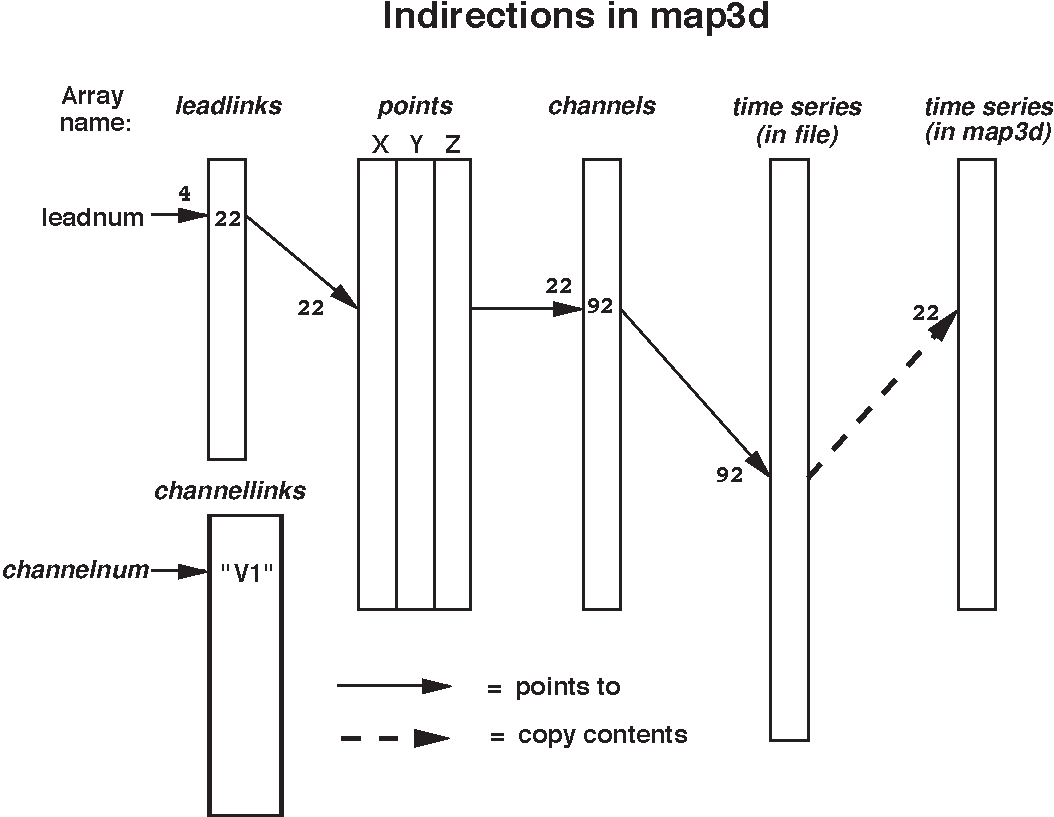
\includegraphics[width=4in] 
      {figures/map3d-indirection.pdf}}}
%end{latexonly}
\begin{htmlonly}
  \newcommand{\ethphoto}{%
     \htmladdimg[align=top,alt="indirection"]
                {figures/map3d-indirection.pdf}}
\end{htmlonly}


\section{Input files}

%% -*-latex-*-
% Document name: defaultfile.tex
% Creator: Rob MacLeod [macleod@cvrti.utah.edu]
% Last update: September 4, 2000 by Rob MacLeod
%    - created but not included in version 1.0 of the manual
%%%%%%%%%%%%%%%%%%%%%%%%%%%%%%%%%%%%%%%%%%%%%%%%%%%%%%%%%%%%%%%%%%%%%%
\subsection{Default settings files}
\label{sec:defaults} 

\map{} looks for files containing default settings for
many parameters that are relevant to the control of the program.
The order of precedence is as follows:
%
\begin{enumerate}
  \item The {\tt-df filename} option defines the file with highest
        precedence default settings.
  \item A file named {\tt .map3drc} in the current directory (the one from
        which the application was launched) is used next.
  \item If no {\tt .map3drc} files is found in the current directory, it is
        searched for in the user's home directory (see the HOME
        environmental variable).  This file has the lowest precedence and
        is only used of the other two options are not found.
  \item The program \map{} has a set of internal defaults which are used
        if there are no external default files found.
\end{enumerate}

\newpage
The format of the default file is as follows:
%
\begin{verbatim}
           # comment line (ignored by map3d)
           parameter = value
\end{verbatim}

\noindent
where the parameters and values are taken from the following list:

\begin{center}
\begin{tabular}{|l|l|p{3.2in}|} \hline
\multicolumn{1}{|c|}{Parameter} &
\multicolumn{1}{|c|}{Values} &
\multicolumn{1}{|c|}{Meaning} \\ \hline
shadingmodel & GOURAUD & Use Gouraud shading of triangles \\ 
             & FLAT    & Use flat shading of triangles \\ \hline
scale\_scope  & GLOBAL\_SURFACE & Scaling global over each surface \\ 
             & GLOBAL\_FRAME   & Scaling global over each frame of data \\
             & GLOBAL\_GLOBAL  & Scaling global over all data \\
             & LOCAL          & Scaling local to each frame and surface\\
             & USER           & Scaling by user-supplied values (-pl -ph)
             \\
\hline
scale\_model  & LINEAR & Use linear scaling of contours \\
             & LOG    & Use logarithmic scaling \\
             & EXP    & Use exponential scaling \\
             & LAB7   & Use logarithmic in 7 levels scaling \\
             & LAB13  & Use logarithmic in 13 levels scaling \\ 
\hline
scale\_mapping & SYMMETRIC & scale symmetrically around both side of zero\\
              & SEPARATE  & scale separately for + and - data values\\
              & TRUE\_MAP  & scale from most - to most + values\\
\hline
color\_map     & RG       & Use full red-to-green colour map \\
              & RG2      & Use red-and-green (2-colour) colour map \\
              & FULL     & Use blue-to-red (full) colour map \\
              & BTW      & Use black-to-white colour map \\
              & WTB      & Use white-to-black colour map \\
\hline
lead\_marking\footnotemark 
              & LEADS          & mark nodes with lead (channel)
                                                             numbers\\ 
              & NODES          & mark nodes with node numbers\\
              & VALUES         & mark leads with potential values\\
              & CUBES          & mark leads with spheres/cubes \\
              & MINMAX\_LABELS & mark extrema with lead numbers \\
              & MINMAX\_CUBES  & mark extrema with cubes \\
              & SCALAR         & mark the selected scalar node \\
\hline
num\_cols      & value    & number of colours to use in shade display\\ \hline
num\_conts     & value    & number of contour levels in display\\ \hline
draw\_bbox     & TRUE/FALSE & set bounding box on or off \\ \hline
datafile\_path & pathame  & alternate path to the .pak/.raw files 
in .tsdf file. \\ \hline
geomfile\_path & pathame  & alternate path to the .geom files 
in .tsdf file. \\ \hline
report\_level  & value    & level of error reporting ( 0--3 ) \\ \hline
\end{tabular}
\end{center}

\footnotetext{options are cumulative} 

Note that these parameters and values are not case sensitive and that they
can all be overridden during execution of the program, typically via the
mouse menu (right mouse button).  See section~\ref{sec:scaling} for details
on the different scaling options.  The list of parameters possible will
also certainly grow with the program.

To save the current settings in a file, there is an option in the main menu
of \map{} which dumps all the settings to the file {\tt ./.map3drc}, that
is, the file {\tt .map3drc} in the current directory.  That way, when you
start the program again from that directory, the same settings will be loaded.
The {\tt .map3drc} file is just a normal text file, but like all
``rc''-files, it is hidden from the {\tt ls} command unless you add the
{\tt -a} option (the alias {\tt la} is set up by default to do a long
listing of all files, including hidden files).  Dumping a copy of the
settings is also the easiest way to see what settings are currently being
maintained by \map{} and also forms the best starting point to setting up
your own customized default settings files.

 %?? Uncomment and update once this feature is working

In this section, we describe the contents and formats of all the input
files that \map{} uses to get geometry, data, and much more.

%%%%%%%%%%%%%%%%%%%%%%%%%%%%%%%%%%%%%%%%%%%%%%%%%%%%%%%%%%%%%%%%%%%%%%

\subsection{Geometry input files}
\label{sec:geomfiles} 

The input of geometric data for \map{} occurs via files and we support
three different formats at present.  The simplest (and oldest) is a set of
ASCII files that contain the points or nodes of the geometry---stored in a
file with the extension .pts---and the connectivities that described
polygonal links between nodes---stored as line segments (.seg files),
triangles (.fac files), and tetrahedra (.tetra files).  To satisfy a need
for more comprehensive and compact storage of geometry information, we have
developed a binary file format and created the \graphicsio{} library to
manage these files.  Finally, in recognition of the ubiquity of MATLAB, as
of version 6.1, there is support for reading .mat files, which have an
internal structure that included node and connectivity information.  Below,
we describe each of these files and how \map{} uses them.

\subsubsection{Points (.pts) file}

The characteristics of a .pts file are as follows:
%
\begin{enumerate}
  \item ASCII file, no special characters permitted;
  \item Each line contains one triplet, ordered as x, y, and z values; one
        or more spaces between values, which are assumed to be real, 
        floating point numbers; 
  \item Each line may also optionally contain a group number as a fourth 
        element (although at present, \map{} does not use this group
        information); 
  \item the order of points in the file is the implicit order of the nodes in
        the geometry; connectivities are based on this ordering.
\end{enumerate}


\subsubsection{Triangle (.fac) files}

The characteristics of a .fac file are as follows:
%
\begin{enumerate}
  \item ASCII file, no special characters permitted;
  \item Each line contains a triplet of integer values pointing to the
        nodes of the geometry.  \textbf{Node numbers begin at 1 not 0!};
  \item The order of triangle vertices (nodes) is not strictly controlled,
        however, it is recommended that order reflect a common convention
        in graphics---a counterclockwise sequence of vertices when viewed from
        the {\bf outside} of the triangle;
  \item Each line may contain an optional fourth values which is the group
        number for the triangle (not used by \map{});
  \item Order of triangles in the file is not meaningful except for
        internal bookkeeping; user will notice ordering only when a
        triangle is picked for interrogation.
\end{enumerate}

\subsubsection{Binary (.geom) geometry files}
\label{sec:geomfile}


At the \htmladdnormallink{CVRTI} {http://www.cvrti.utah.edu} we have
developed a binary file system for efficient storage of complex geometry
and associated attributes, a part of what we call the \graphicsio{}
library.  Extensive documentation of this format is available from \rob{}
(\htmladdnormallink{www.cvrti.utah.edu/\~{}macleod/docs}
{http://www.cvrti.utah.edu/~macleod/docs}).

Briefly, each \graphicsio{} geometry file contains one or more sets of
node locations and, optionally, connectivities for polygonal elements
composed from those nodes.  It is possible in \graphicsio{} files to
associate scalar, vector, and tensor values to nodes or elements, the
most relevant example of which are channel pointers, stored as a set of
scalar values associated with the nodes of the geometry.  Each 
\graphicsio{} geometry file can contain any number of sets of 
geometries, each with different nodes and connectivities.  A typical
example for \map{} would be a single .geom file that contains information
from multiple surfaces that we might want to display together.


\map{} is capable of reading surface geometry from either single surfaces
or from all surfaces contained in a multi-surface geometry file. 
Command line arguments controls the selection, as we describe in the next
section.

\subsubsection{MATLAB geometry file support}
\label{sec:matlabgeom}

\map{} can read .mat files generated by MATLAB as long as they are
organized according to the following guidelines:
\begin{enumerate}
  \item Each separate surface is either a structure (See 
    the MATLAB documentation for 
%\htmladdnormallink{cells}
%    {http://www.mathworks.com/access/helpdesk/help/techdoc/matlab_prog/ch_da37a.html#67323}
%    and  
    \htmladdnormallink{structures}
    {http://www.mathworks.com/access/helpdesk/help/techdoc/matlab\_prog/ch02\_d27.html\#88951}
     ).  To include multiple surfaces requires an array of
    structures.
  \item Within a surface structure, the following fields contain the
    geometry:
    \begin{itemize}
      \item \emph{.pts or .node} contains the node locations, usually in a
        $3 \times N$ array (although \map{} will check and accept either $3
        \times N$ or its transpose, $N \times 3$), where $N$ is the number
        of nodes.
      \item \emph{.fac or .face} contains the triangle connectivities,
        usually in a $3 \times M$ array (again, \map{} will accept the
        transpose)\, where $M$ is the number of triangles.
      \item \emph{.seg or .edge} contains the line segment connectivities,
      \item \emph{.tet, .tetra, or .cell} contains tetrahedral
        connectivities, and
      \item \emph{.channels} contains the channel information in a
        one-dimensional vector, in which each element of the vector points
        to the associated data channel.
    \end{itemize}
\end{enumerate}

To prepare a structured .mat file is very simple, for example using the
following commands:
%
\begin{verbatim}
     >> geom.pts = ptsarray;
     >> geom.fac = facarray;
     >> geom.channels = 100:164
     >> save mygeom.mat geom
\end{verbatim}
%
where \verb|ptsarray| is a $3 \times N$ array defined to contain the node
locations, \verb|facarray| is a $3 \times M$ array of triangle
connectivities, and \verb|mygeom.mat| is the name of the resulting .mat
file.   The channels information indicates that there are 64 nodes in the
geometry and they expect to get time signals from channels 100--164 of a
data file.  (See Section~\ref{sec:leadfiles} for more information on
channels. 

\subsubsection{Landmark geometry file support}
\label{sec:landmarkgeom}

\map{} can also read geometry from a landmark file 
(See Section~\ref{sec:lmfile} below), where you specify a series
of connected points and radii.  \map{} will automatically connect
and triangulate them, and will also associate scalar data with them.
Note that currently there is no channels support for landmark geometry.


%%%%%%%%%%%%%%%%%%%%%%%%%%%%%%%%%%%%%%%%%%%%%%%%%%%%%%%%%%%%%%%%%%%%%%

\subsection{Command line control of geometry files}
\label{sec:readgeom}


In \map{} the -f option determines in which files the geometry is to be
found.  Starting from the filename that follows -f, which may or may not
include a file extension, the program looks for all possible candidate
geometry files and queries the user for resolution of any ambiguities.
Thus, with the arguments {\tt map3d -f myfile}, \map3d{} looks for
\texttt{myfile.geom}, \texttt{myfile.mat}, \texttt{myfile.pts},
\texttt{myfile.fac}, \etc{} and tries to resolve things so that a valid
geometry description is found.  It is possible to direct this process by
typing the geometry filename with an extension according to the following
rules:
%
\begin{center}
\begin{tabular}{|l|p{4in}|} \hline
\multicolumn{1}{|c|}{Extension} &
\multicolumn{1}{|c|}{Effect} \\ \hline
none & look for files with the extensions .pts, .fac, .tetra, and .geom and
if an incompatible set are present (\eg{} both .pts and .geom), ask user
which to take \\ 
.pts & take only the .pts file and ignore any connectivity or .geom file \\
.fac & take .pts and .fac and ignore any .geom files present. \\
.geom & take the graphicsio geometry file and ignore any others present. \\
.mat & take the MATLAB file and ignore any others present. \\ \hline
\end{tabular}
\end{center}

A further way to read geometry into \map{} is to use the geometry filename
that can be optionally contained within the time series file (see
Section~\ref{sec:datafiles}) that contains the potentials.  This requires
that the .tsdf file be created with the geometry filename
included; adding this after the fact is difficult.  Note that even if a
geometry filename is found in the .tsdf file, it can be overridden
by the geometry file name specified in the argument list of \map{}.

%%%%%%%%%%%%%%%%%%%%%%%%%%%%%%%%%%%%%%%%%%%%%%%%%%%%%%%%%%%%%%%%%%%%%%

\subsection{Scalar data files}
\label{sec:datafiles} 

There are three ways of storing scalar values (typically electric potential
in our applications) so that \map{} can recognize and read them.  One is a
simple ASCII file, one is a binary format developed at the
CVRTI\@, and the third is MATLAB. 

\subsubsection{.pot files}
\label{sec:potfiles} 

One way to package the scalar data values that are assigned to the points
in the geometry is the .pot file.  In the default condition,
the scalar values in the .pot files are ordered in the same way as
the node points in the geometry file with simple one-to-one assignment.
With a channels file, it is possible to remap this assignment, as described
in Section~\ref{sec:leadfiles}).

\noindent
The rules for .pot files are:
%
\begin{enumerate}
  \item Each line of the files contains one scalar data value, assumed to
        be a real number in single precision floating point format. 
  \item The order of the values within the file must either agree with that
        of the associated set of nodes or a channels file must be supplied
        to redirect the links between potential value and nodes.
  \item Each .pot file {\em must\/} end with a blank line.
  \item A single .pot file can contain only the data values
        associated with a single surface at a single instant in time.  To
        represent a sequence of time steps (frames) requires a sequence of
        files, typically with filenames ending in a three-digit series,
        \eg{} \texttt{mapdata001.pot}, \texttt{mapdata002.pot},
        \texttt{mapdata003.pot}, \ldots{}.  Section~\ref{sec:scalarparams}
        explains how to specify such a series of .pot files to \map{} and
        Section~\ref{sec:usage-examples} shows examples.
  \item The extension .pot {\em must\/} be used.
\end{enumerate}


\subsubsection{CVRTI data (.tsdf and .tsdfc) format files}
\label{sec:tsdffile} 

One efficient and flexible way to store scalar values is by means of the
time-series data file format developed at the CVRTI, also as part of the
\graphicsio{} library.  Each time series data file (.tsdf files) holds an
entire sequence, or \emph{time series} of scalar data in a single file,
along with some information about the contents, type, units, and global
(\ie{} that apply to all channels) temporal fiducials from the time series.
For more details on this file format see
\htmladdnormallink{www.cvrti.utah.edu/\~{}macleod/docs/graphicsio}
{http://www.cvrti.utah.edu/~macleod/docs/graphicsio}.

Here are some concepts of the time series data file structure that are
relevant to the different modes of operation described in this manual.
%
\begin{description}
  \item [Links to geometry]  The
        links between the channels of data in the .tsdf file and the nodes
        of the surface[s] over which they are displayed is established via
        {\em channel\/} array information, which is available stored as
        associated scalars to the nodes in the geometry file (see
        Section~\ref{sec:geomfiles}) or in explicit channels files (see
        Section~\ref{sec:leadfiles}).
  \item [Frames]  By {\em frames\/} of data, we mean instants in the data
        stream representing single moments in time.  For each frame, there
        is a set of values that for a spatial distribution or map and
        \map{} needs to know what subset of frames are to be 
        included in the display.  To explicitly specify frame numbers, use
        the \texttt{-s} and \texttt{-i} options described in
        Section~\ref{sec:usage}.  As an example, the command line
\begin{verbatim}
        map3d -w -f geomfile.geom@1 -p datafile.tsdf -s 10 130 -i 2
\end{verbatim}
        specifies that surface 1 from the geometry file {\tt geomfile.geom}
        should be used to display frames 10 to 130, taking every second
        frame, from run 2 of the time series data file {\tt datafile.tsdf}.
\end{description}


\paragraph{Time series container files (tsdfc): } 
\label{sec:tsdfcfile}

There is an extension to the \graphicsio{} library that defines a container
file format for a set of time series data (.tsdf) files, and
can contain parameters extracted from the associated time series.  These
files are actually small databases and we use a modified (patched actually)
version of the GNU Database Library (GDBL) to manage them.  

Examples of programs and libraries that provide support for .tsdfc
files include Everett, a program by Ted Dustman for initial processing of
mapping data,  \htmladdnormallink{Matmap}
{http://www.cvrti.utah.edu/~jeroen/matmap/}, a set of MATLAB uilities by
Jeroen Stinstra with a similar functionality, and \texttt{tsdflib} (as yet
undocumented), a library created by Ted Dustman, Rob MacLeod, Jenny
Simpons, and Jeroen Stinstra that provides C-language access to container
files.

For more information on container files, see the documentation for the
graphicsio library at
\htmladdnormallink{www.cvrti.utah.edu/\~{}macleod/docs/graphicsio/}
{http://www.cvrti.utah.edu/~macleod/docs/graphicsio/}. 

\subsubsection{MATLAB data file support}
\label{sec:matlabdata}

You can also store and read scalar values in .mat files, as a structure
with a single field called ``.potvals'', that contains a $N \times M$ array,
where $N$ is the number of data channels and $M$ is the number of time
instants.  There are additional fields in the structure that mimic the
information available in the graphicsio .tsdf file so---the complete list is
as follows:
%
\begin{itemize}
  \item \emph{.potvals, .data, .field, or .scalarfield} scalar values as $N
    \times M$ array, where $N$ is the number of data channels and $M$ is
    the number of time instants.
  \item \emph{.unit} the type of units for the data, ``um'' for microvolts,
  ``mv'' for millivolts and ``V'' for volts.
  \item \emph{.label} the name of the time series.  This is optional, but is
    useful in identifying the time series, particularly from a 
    multi-time-series file.
  \item \emph{.fids} a structure (or array of structures) containing
    fiducial time markers for the time series (see below for details of
    fidicual storage).
\end{itemize}

Note that only the 'potvals' field is required.  A matlab array may 
be one instance of these fields, a cell or struct array of them, or 
simply an $N \times M$ array of data.  To read a matlab file with many time
time series, specify the time series on the command line with the '@' symbol
(See Section~\ref{sec:scalarparams}) or specify the time series in the 
file browser.  It will be shown by the label specified in the matlab file.

The commands to make a suitable .mat file are very easy in MATLAB, for
example, to load 128 channels of time signals with unit of millivolt from
an array \texttt{sockinfo} in MATLAB to a file called
\texttt{mysockdata.mat}
%
\begin{verbatim}
    >> sockdata.potvals   = sockinfo(1:128,:);
    >> sockdata.unit = 'mV'
    >> sockdata.lavel = 'A set of cool sock data'
    >> save mysockdata.mat sockdata
\end{verbatim}

\subsubsection{Fiducial (ascii) files}
\label{sec:fidfiles}

A fiducial can be input currently also in three ways: via a .tsdfc file,
where the potential and fiducial values are stored together, via a .fids
file, a simple ASCII file containing the values for each node, or by means
of the MATLAB file that contains the time series data.

\paragraph{MATLAB file format for fiducials}


The fiducial information in a MATLAB time series data file is stored in a
array of structures called fids, where each element of the array represents
one set of fiducials.  This way, for example, there can be a set of $N$
activation times, another set of $N$ recovery times, and a set of $N$
Q-onset times.  Each element of the array is, in itself, a structure, so
that the set of fiducials contains enough information for \map{} to do a
useful display. 

The legal elements of a fids structure are as follows:
%
\begin{itemize}
  \item \emph{.type} the type of fiducial (see table below).
  \item \emph{.value} the array of fiducial values, one for each 
    channel of the data file.
\end{itemize}


Here is an example of creating the structures for some fiducials in MATLAB:
%
\begin{verbatim}
   matdata.potvals = potvals;
   matdata.unit = unit;
   matdata.label = label;
   matdata.fids(1).type = 10
   matdata.fids(1).value = fidvals(:,1);
   matdata.fids(2).type = 13;
   matdata.fids(2).value = fidvals(:,2);
   save (outfilename, 'matdata');
\end{verbatim}

The first three lines set up the time series data, as we have seen above.
The lines 4 and 5 create a set of fiducials of type 10 and loads the values
into that part of the data structure.  Lines 6 and 7 do the same thing for
a second set of fiducials, which have type 13. The final line saves the
contents of the structure into a file.

The type value for fiducials is important as \map{} associates colors to
fiducial types to provide consistent display.  Moreover, each type has an
associated text label that \map{} uses in the interface.  The list of
current fiducial types and their numbers is as follows:

\bigskip

\begin{center}
\begin{tabular}[h]{|c|l|} \hline
\multicolumn{2}{|c|}{Fiducial Types} \\  \hline \hline
Number & Type \\ \hline 
 0 & pon, pstart \\
 1 & poff, pend \\
 2 & qon, qrsstart, qrson \\
 3 & rpeak, qrspeak \\
 4 & soff, qrsend, qrsoff \\
 5 & stoff, tstart, ton \\
 6 & tpeak \\
 7 & toff \\
 8 & actplus \\
 9 & actminus \\
 10 & act \\
 11 & recplus \\
 12 & recminus \\
 13 & rec \\
 14 & ref, reference \\
 15 & jpt, jpoint \\
 16 & baseline \\
 30 & pacing \\
\hline
\end{tabular}
\end{center}

\paragraph{ASCII file format for fiducials}

The characteristics of a .fids file are as follows:
\begin{enumerate}
  \item ASCII file
  \item must have the following at the top of the file, on each line:
  \begin{enumerate}
    \item number of time series, e.g., 1 (\map{} only allows 1)
    \item series number (space) pak number
    \item number of nodes (space) list of fiducial types
  \end{enumerate}
  \item each successive line contains the node number followed by
        a list of fiducial values, one corresponding to each
        type specified on the line with the node numbers
\end{enumerate}

\begin{verbatim}
    Example:
    1
    1 -1
    256 activation recovery
    1 8 212
    2 16 225
    3 9 214
    ...
    255 39 248
    256 25 237  
\end{verbatim}


%%%%%%%%%%%%%%%%%%%%%%%%%%%%%%%%%%%%%%%%%%%%%%%%%%%%%%%%%%%%%%%%%%%%%%

\subsection{Channels and leadlinks}
\label{sec:leadfiles} 

\subsubsection{Description of leadlinks and channels
information}

Channels and leadlinks files, and the arrays they
contain, are identical in structure, but they have important {\bf
functional differences}.  A run of \map{} may require both, either, or
neither of these, depending on the structure of the data files and
geometries. The basic function of both channels and leadlinks information
is to offer linkages between nodes in the geometry and the data that is to
be associated with those nodes.  The first file type, the channels file,
links the nodes in the geometry to specific time signals in a data file;
without channel mapping, the only possible assumption is that each node $i$
in the geometry corresponds to the same time signal $i$ in the data file.
Any other linkage of geometry and data channel requires there to be channel
information, typically either from a separate .channels file or stored with
the binary .geom file as an associated scalar value for each node.

\begin{figure}[htb]
   \begin{makeimage}
    \end{makeimage}
    \indirec
    \caption{\label{fig:indirec}Example of the indirection possible in
      \map{} through the use of {\em leadlinks\/} {\em channels}, and {\em
        channellinks}.  Lead number 4 points, via the {\em leadlinks\/}
      array to node number 22.  This, in turn, points via the {\em
        channels\/} array to location 92 in the multiplexed data buffer,
      which causes the values at time signal 92 to be loaded into location
      22 in the internal data array (and displayed by \map{}).  In a
      separate, \emph{channellinks} array, shown below the leadlinks array,
      the entry in lead 4 says that that lead should actually be labeled
      ``${\rm V_{1}}$''. }
\end{figure}

Leadlinks are purely for visualization and describe the connection between
``leads'', a measurement concept, with ``nodes'', a geometric location in
space.  In electrocardiography, for example, a lead is the algebraic
difference between two measured potentials, one of which is the reference;
``unipolar'' leads have a reference composed of the sum of the limb
electrode potentials.  It is often useful to mark the locations of these
leads on the geometry, which often contains many more nodes than there are
leads.  The most frequent use to date has been to mark the locations of the
standard precordial ECG leads within the context of high resolution body
surface mapping that uses from 32--192 electrodes.  Another common
application is to mark subsets of a geometry that correspond to 
measurement sites (values at the remaining nodes are typically the product
of interpolation).  In summary, leadlinks allow \map{} to mark specific
nodes that may have special meaning to the observer.

Figure~\ref{fig:indirec} shows an example of lead and channels
information and their effect on \map{}.  See the figure caption for
details. 


\map{} handles this information in the following manner:
%
\begin{description}
  \item [channels]  The {\em channels\/} information links 
        nodes in the geometry to individual channels or time series in the
        data file.  For example, the data values associated with node
        $k$ in the geometry are located in the data location specified by
        the channel array value ${\rm channels}(k)$.  If ${\rm channels}(k)
        < 0$, then there is no valid data for node $k$.

        Note that \textbf{ \map{} uses the channels arrays when
        loading scalar data into the internal storage arrays!}  Hence, the
        action of the channel mapping is not reversible.   Should geometry
        nodes and data channels match one-to-one, there is no need for a
        channels array.  It is also possible to define via a channels array
        the situation in which a single data channel belongs to two (or
        more) nodes in the geometry.  The most frequent example of this
        occurs when three-dimensional geometries are ``unwrapped'' into
        surfaces in which what was a single edge is split and thus present
        at both ends of the surface.

  \item [leadlinks] The {\em leadlinks\/} information is primarily
        used to identify and mark measurement lead specific within the
        geometry.  The typical use is to select a subset of the nodes to
        identify the measurement sites---values at other sites might
        be interpolated or otherwise computed.  Leadlinks also provide a
        means to renumber the labels on the nodes of the geometry in order
        to, for example, reproduce the numbering scheme used in an
        experimental setup.
        
        In the leadlinks array each entry refers, by its location in the
        array, to a particular lead \#; the value at that location in the
        array gives the number of the node in the geometry file to be
        associated with this lead.  For example if lead 4 has a leadlinks
        entry of 22 (${\rm leadlinks}(4)=22$), then \map{} will display
        node 22 in the geometry as ``4'', not ``22'' whenever node marking
        with \emph{leads} is selected).

  \item [channellinks] There is an extension of the basic scheme which
        includes a further level of redirection for giving the leads
        explicit text labels.  Channel links are stored as a array of
        strings, one for each node of the geometry.  The channellinks file
        is organized similarly to a leadlinks file, with each line
        containing information for one node.  However, each line consists
        of two values, 1) the number of the associated channel and 2) the
        text string to be used as the label when \map{} marks the nodes
        with channel numbers.
        
        Hence we have the situation of a node number $K$ in the geometry 
        displaying time signals from channel $L$ in the scalar data, but
        labeled with string ``XXX''. 

\end{description}

\subsubsection{Source of leadlink and channel information}

The sources of channels, leadlinks, and channellinks information are
files, or parts of files, as outlined in the following paragraphs.

\paragraph{In .geom files}

Information for the {\em channels\/} array is stored as an associated
scalar with the information in the standard .geom files.  At
present, there is no leadlinks array stored in the .geom file but
this could change in the future.

\paragraph{In .mat geometry files}

MATLAB geometry files can also contain an {\em channels\/} array is stored as
a .channels field in the structure.  See Section~\ref{sec:matlabgeom} for
more details.


\paragraph{In .leadlinks files}

A .leadlinks file is an ASCII file, the first record of which
contains a line {\tt nnn leads}, where {\tt nnn} is the number of leads to
be described in the file (and also one less than the total number of lines
in the file).  Each following record contains two integer values:\\
%
\begin{enumerate}
  \item the first number is the number of the lead, as it should appear in
        any labeling of the associated node.
  \item the second entry in each row is the value of the associated node
        number in the geometry.  
 \end{enumerate}
%
For example, the file for a surface which reads:
%
\begin{verbatim}
    32 Leads
    1   1   
    2   42  
    4   31  
    7   65  
    .   .   
    .   .   
    .   .   
    32  11     <---- 32nd entry in the file, at line 33 of the file.
\end{verbatim}
%
indicates that there are 32 leads to be linked (the geometry can, often
does, contain more than 32 nodes), and that lead \#1 is called lead ``1''
and is node 1 in the geometry file.  Lead \#2 is at node 42, lead \#3 is
called ``4'' and is found at node 31.  Likewise, lead \#4 is called ``7'',
and is located at node 65, and so on, up to lead \#32, called ``32'', at
node 11.

Nodes listed in a {\em leadlinks} file that is passed to \map{} with the
{\tt -ll} option can be marked in a number of ways, described more fully in
Table~\ref{table:nodemarking} in Section~\ref{sec:control-menus}.

\paragraph{In .channels files}

A \emph{channels} file is an ASCII file, the first record of which contain a
line {\tt nnn nodes}, where {\tt nnn} is the number of nodes to be
described in the file (and also one less than the total number of lines in
the file).  There is one line in the file for each node of the geometry to
which we wish to associate scalar data.   Each following record contains
two integer values:\\ 
%
\begin{enumerate}
  \item the first number is simply a running counter that indicates
        the node number with which to associated the second value in the
        row.
  \item The second value in each row is the {\em channel\/} number for
        that node; a negative number signifies a node to which there is no
        data associated.
\end{enumerate}

\noindent
For example, the file for a surface which reads:
%
\begin{verbatim}
    352 Nodes
    1    123
    2    632
    .    .
    .    .
    22   -1
    23   432
    .    .
    .    .
    352  12
\end{verbatim}
%
indicates that there are 352 leads to be linked, and that the data value
for the first node is located at location 123 of the data file.  For node
2, the data value is to be found at location 632, and so on.  Node 22 does
not have any scalar data associated with it.

\subsubsection{Display of lead/channel information}

To see how \map{} can display the node and lead information, see
Sections~\ref{sec:displayleads} and~\ref{sec:control}. 

%%%%%%%%%%%%%%%%%%%%%%%%%%%%%%%%%%%%%%%%%%%%%%%%%%%%%%%%%%%%%%%%%%%%%%

  \subsection{Landmark files}
  \label{sec:lmfile} 

  Landmark files contain information for visual cues or landmarks that \map{}
  can draw over the surfaces in order to aid and orient the viewer. Initial
  use was primarily for coronary arteries, but the idea has expanded to
  incorporate a number of different orientation landmarks.  The original
  coronary artery class of landmarks requires only that each can be described
  as a series of connected points, with a radius defined for each point.  The
  coronary landmark is then displayed as a faceted ``pipe'' linearly
  connecting the points at the centre, with a radius, also linearly
  interpolated between points, determining the size of the pipe.  The
  landmark file can contain numerous, individual segments of such pipe-work,
  each of which is drawn separately.

  Other classes of landmarks are described below, but all of them can be
  described in a file with the following general format:
  %
  \begin{center}
  \begin{tabular}{|l|l|p{3.0in}|}
  \hline
  \multicolumn{1}{|c|}{Line number} &
  \multicolumn{1}{|c|}{Contents} &
  \multicolumn{1}{|c|}{Comments} \\ \hline
  1 & nsegs   & number of landmark segments in the file \\ \hline
  2 & 1 type nsegpts [segindex] [segcolor] & segment number (1), type, number of
  points, with optional index number and color (color is a RGB triple, 0-255 each) \\ 
  3 & X, Y, Z, radius [label] & point location and radius of point 1, with optional label to be drawn at the point \\
  4 & X, Y, Z, radius [label] & point location and radius of point 2 \\
  . & . & . \\
  . & . & . \\
  nsegpts + 2 & X, Y, Z, radius & point location and radius of last point in
                              segment 1 \\ \hline
  . & 2 type nsegpts [segindex] [segcolor] & segment number (2), type, number of
  points, with optional index number and color \\ 
  . & X, Y, Z, radius [label] & point location and radius of point 1 \\
  . & X, Y, Z, radius [label] & point location and radius of point 2 \\
  . & . & . \\
  . & . & . \\
  . & X, Y, Z, radius [label] & point location and radius of last point in
                              segment 2 \\ \hline
  . & . & . \\
  . & . & . \\
  . & . & . \\
  . & . & . \\
  \hline
  \end{tabular}
  \end{center}

  The landmark types defined to date are the following:
  %
  \begin{center}
  \begin{tabular}{|l|p{1.5in}|p{3.5in}|} \hline
  \multicolumn{1}{|c|}{Name} &
  \multicolumn{1}{|c|}{Graph. object} &
  \multicolumn{1}{|c|}{Description}\\ \hline
  Artery & faceted pipe & a coronary artery/vein segment\\
  Occlusion & coloured sphere & an experimental occlusion that could be open and
  closed \\ 
  Closure & coloured sphere & a permanent occlusion that cannot be opened \\
  Stimulus & coloured sphere & a stimulus site \\
  Lead & coloured sphere & a particular electrode or lead location \\
  Plane & rectangular parallolopiped & a visible (but not functional) cutting
  plane through  the geometry (Note: do not confuse this with the cutting
  planes that \map{} provides for slicing through the  geometry).\\
  Rod & lines & rod inserted into needle track to digitize needle electrode
  locations. \\
  PaceNeedle & sphere & location of a pacing needle entry point\\
  Cath & faceted pipe & location of catheter in a vessel \\
  Fiber & arrow & local fiber direction indicator\\
  RecNeedle & sphere & location of recording needle entry point \\
  Cannula & tube & coronary vessel cannulus \\
  \hline
  \end{tabular}
  \end{center}

  Specifying  snare, closure, and stimulus requires a single point in the
  landmarks file, and the resulting sphere is coloured according to a set of
  values defined in the drawsurflmarks.c routine.  At present, the values
  used are:
  %
  \begin{center}
  \begin{tabular}{|ll|} \hline
    Occlusion & cyan \\ 
    Closure & blue \\
    Stimulus & yellow \\ \hline
  \end{tabular}
  \end{center}

  %
  and they are adjustable by the user, either via the Landmark menu, or by
  specifying a color for the segment

  To specify a plane landmark requires three ``points''
  %
  \begin{center}
  \begin{tabular}{|c|l|l|} \hline
    \multicolumn{1}{|c|}{Point} &
    \multicolumn{1}{|c|}{X,Y,Z} &
    \multicolumn{1}{|c|}{Radius} \\ \hline
  1 & First point of plane & Radius of the plane \\
  2 & Second point of plane & Thickness of the plane \\
  3 & Third point of plane & not used \\ \hline
  \end{tabular}
  \end{center}
  %
  The plane is drawn as a polygon with the number of sides controlled by a
  program variable. 

\paragraph{Filename conventions: } The standard extension of a
  landmark file is {\tt .lmarks} and the filename is specified by the {\tt
  -lm} parameter for each surface.

\paragraph{Control of landmark display: } for details of how to control the
display of landmarks, see Section~\ref{sec:control-landmarks}.



%%% Local Variables: 
%%% mode: latex
%%% TeX-master: "manual"
%%% End: 

\newpage
% -*-latex-*-
% Document name: display.tex
% Creator: Rob MacLeod [macleod@vissgi.cvrti.utah.edu]
% Last update: September 2, 2000 by Rob MacLeod
%    - created
% Last update: Sun Sep 24 22:24:02 2000 by Rob MacLeod
%    -  Version 5.0Beta release edition
% Last update: Mon Jul 23 13:28:30 2001 by Rob MacLeod
%    - release 5.2
% Last update: Fri Jun 21 13:35:32 2002 by robmacleod
%    - late update for release 5.3
% Last update: Wed Mar 31 13:35:32 2004 by Bryan Worthen
%    - late update for release 6.0
% Last update: Wed Jun 30 13:28:30 2004 by Bryan Worthen
%    - release 6.1
% Last update: Wed May 11 13:28:30 2005 by Bryan Worthen
%    - release 6.3
% Last update: Fri Feb 16 09:15:56 2007 by Rob Macleod
%    - version 6.5
%%%%%%%%%%%%%%%%%%%%%%%%%%%%%%%%%%%%%%%%%%%%%%%%%%%%%%%%%%%%%%%%%%%%%%
%%%%%%%%%%  Figures used in this file %%%%%%%%%%%%%%%%%%%%%%%%%%%%%%%%
%begin{latexonly}
  \newcommand{\timesignal}%
  {\centerline{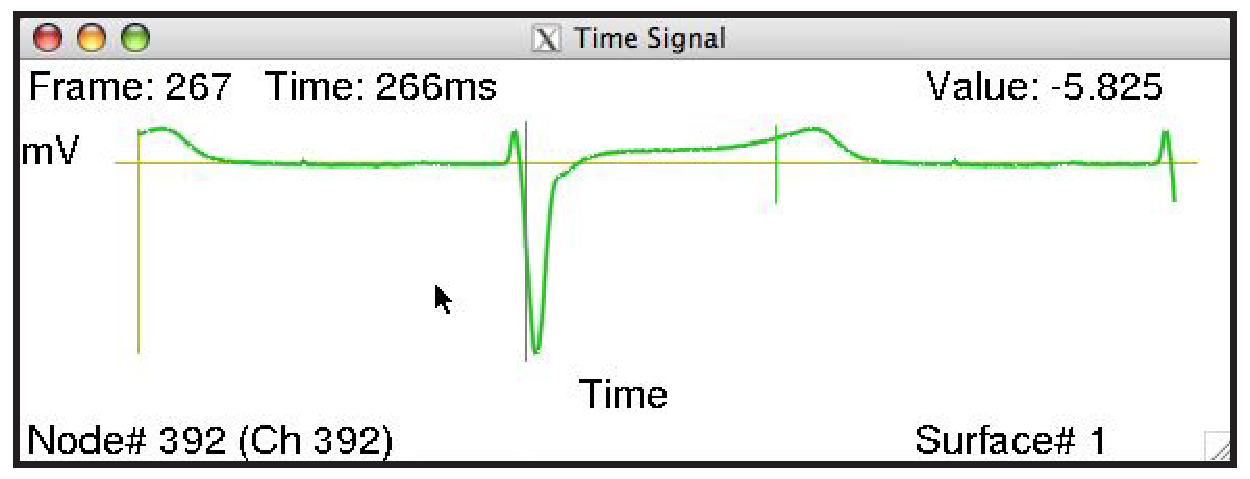
\includegraphics[height=2in]{figures/timesignal.pdf}}}
%end{latexonly}
\begin{htmlonly}
  \newcommand{\timesignal}{%
  \htmladdimg[align=top,alt="time signal"]
  {../figures/timesignal.jpg}}
\end{htmlonly}
%%%%%%%%%%%%%%%%%%%%%%%%%%%%%%%%%%%%%%%%%%%%%%%%%%%%%%%%%%%%%%%%%%%%%%

\section{Display features}
\label{sec:display} 

This section describes the displays that \map{} generates and what they
mean; for specific information on how to control \map{} and the displays,
see Section~\ref{sec:control}.

\subsection{Multiple surfaces}
\label{sec:displaysurfaces} 

The idea of \map{} has always been to display multiple sets of data on
multiple surfaces; the limitation has been how much flexibility to include
in a single invocation of the program.  This version of \map{}, as opposed
to previous versions, can now handle multiple windows each with multiple
surfaces.  Surfaces can be moved between windows (see
Section~\ref{sec:fileswindow}) When \map{} displays multiple surfaces, each
can exist in its own full window with its own border and window title bar,
or, \map{} can build a single main window with multiple sub-windows inside
the main window.  The user can reposition and resize each of these
sub-windows using the Alt(Meta) key and the left and middle mouse buttons
respectively.  To create this layout of main window and frameless
sub-windows, use the \texttt{-b} (borderless windows) option when launching
\map{} as described in Section~\ref{sec:usage-geometry}.


\subsection{Surface display }

The basic forms of display of the surfaces are
%
\begin{itemize}
  \item nodes or points from each surface
  \item connectivity mesh
  \item shaded surfaces based on either the geometry or the associated
        scalar values, with a number of different rendering options.
  \item landmarks superimposed on the surface display
\end{itemize}

%%%%%%%%%%%%%%%%%%%%%%%%%%%%%%%%%%%%%%%%%%%%%%%%%%%%%%%%%%%%%%%%%%%%%%

\subsection{Mesh Rendering}
\label{sec:display-mesh} 

Often the purpose of \map{} is to render a geometry consisting of nodes and
connectivities and there are several basic modes of rendering this
information. 

\begin{description}
  \item [Points: ] display just the nodes of the geometry as dots or marked
        with spheres.
  \item [Connectivities: ] display the connectivity information for the
        mesh as lines joining the nodes.
  \item [Elements: ] treat each polygon in the mesh as an element and
        render it in a way that shows its surface; for triangles, simple
        render each triangle surface; for tetrahedra there is no specific
        rendering in this version of \map{}.
  \item [Elements and connectivities: ] \map{} also supports a hybrid mode
        of rendering that shows outward facing triangles (using the
        convention of counterclockwise ordering) as elements but backwards
        facing triangles as connectivities.
\end{description}

\map{} also has the ability to render
all elements with a lighting model.  This is especially useful for
displaying the elements of the mesh.  Additional controls to note are depth
cueing, which can reveal the depth relationships between elements of the
mesh. 

%%%%%%%%%%%%%%%%%%%%%%%%%%%%%%%%%%%%%%%%%%%%%%%%%%%%%%%%%%%%%%%%%%%%%%

\subsection{Surface Data Display} 
\label{sec:display-data} 

The main use of \map{} is to display scalar data associated with geometry
and there are numerous options and controls to facilitate this.  The two
basic ways of conveying scalar value information are as shaded surfaces
and contour lines and \map{} supports each separately, as well as in
combination.  For surface shading, there are several basic rendering modes:

\begin{description}
  \item [Flat: ] each triangle received a single color that depends on the
        mean value of the scalar value over that triangle.
  \item [Gouraud: ] the colour of each triangle values linearly with the
        value at each of the vertices.  The current version uses texture
        mapping to achieve more desirable results, but if your hardware
        does not support texture mapping, you can toggle it with the g-key.
  \item [Banded: ] the regions between contour lines have a constant color,
        even if the contour lines are not visible.
  \item [Contours: ] this can be a separate rendering mode, or combined
        with any of the three modes above.  Contours are lines that trace
        iso-values over the surface of the geometry.
\end{description}


\subsubsection{Data scaling}
\label{sec:scaling} 

There is a wide variety of options available for mapping scalar values to
colour and contour levels.  One can picture the process as based on four
facets: 

\begin{description}
  \item [Extrema: ] the extrema of the data and the selected colour maps
        determine the basic parameters of how value maps to color.  \map{}
        maintains a detailed list of data extrema organized both by time
        signal, time instant and by surface.  Thus it is possible to determine
        extrema based on just the most local of conditions---a particular
        frame and surface---or by more global conditions---the full range
        of frames or the full set of surfaces.
  \item [Scaling function: ] the mapping between value and color occurs
        according to some mathematical function, the simplest of which
        is linear.   The scaling function uses the selected extrema and
        describes a complete mapping between value and color.
  \item [Mapping: ] by scale mapping, we mean how the translation from
        value to color treats positive and negative values.  We may choose
        to map uniformly between the extrema or to apply different
        extrema or functions to the positive and negative values.
  \item [Color maps: ] the color displayed for a particular scalar value
        depends on the actual range of colors and their order in the color
        map.
\end{description}

\map{} can adjust all four facets of the scaling to create a wide range of
displays.  Note that all surfaces conform to the first three scaling
options (there is only one scaling range, function, and mapping that
corresponds to all surfaces).  We also chose to limit some of these 
options, however, in an effort
to create reproducible displays that reflect standard within the field.  Of
course, we chose our field, electrocardiography, as the basis, a fact for
which we make no apologies and simply encourage others to make similar
choices for their own field and implement \map{} accordingly.  Subsequent
versions of \map{} will support this flexibility.

Below are the specific choices that \map{} offers to control data scaling
and display
\begin{description}
  
  \item[Scale range] \map{} supports several selections of range over which
    to look for extrema.  In {\em local\/} range, only the data presently
    visible are scanned for extrema---this is the default.  In the full
    {\em global\/} range, all the data in the entire dataset are used, even
    those not presently visible on the display.  In between these cases,
    one can have global in time and local in space, \ie{} we scale each
    surface separately but use all time values for that surface.  Or one
    can select local in time and global in space, in which \map{} scans all
    surfaces for the data extrema, but for each time instant separately.  

    The user can also select group
    scaling, where he assigns surfaces to groups and the range is based on
    the group min/max (either local in time or global).  Groups are
    assigned by the menu.  The user can also do slave scaling, where he
    assigns one surface (slave) to another's (master) range.  The slave
    surfaces are currently only set through the command line, by placing a
    -sl num (where num is the surface number of the master) after declaring
    the slave surface.  See Section~\ref{sec:control-menus} and
    Section~\ref{sec:scalarparams} for details.

    If these options are not suitable, the user can select his own scaling 
    scope for
    maximum and minimum values. This can be set via the command line 
    (see {\tt -pl} and {\tt -ph} input parameters in Section~\ref{sec:usage}).
    or in the Contour Spacing dialog (see Section~\ref{sec:contourwindow}).
    While the rest of the scaling range options are set once for all 
    surfaces, whether or not an individual surface corresponds to the
    default range can be selected through the Contour Spacing dialog as well.

        
  \item[Scale function] The scale model describes the way in which scalar
    data are mapped to colours (or contours).  The present choice is
    linear, but the next version of \map{} will include: \textbf{linear}
    model, which simply maps the data to a range of colours in a completely
    linear fashion, \ie{} \mbox{$colour = K \phi$}; the
    \textbf{logarithmic} model, which highlights the lower level data
    values at the cost of poorer resolution at the higher levels \ie{}
    \mbox{$colour = A\log(\phi) + B$}; and the \textbf{exponential} model,
    which does the opposite, compressing the smaller levels and expanding
    the higher ones to span a wider colour range, \ie{} \mbox{$colour = A
      e^{B\phi}$}.
    
    The two schemes with fixed numbers of contours, {\em log/7-levels\/}
    and {\em log/13-levels\/} both map the upper decade ($\phi_{max}$ to
    $\phi_{max}/10.$) of the potential data range into a fixed set of
    logarithmically spaced values.  These values are composed of a mantissa
    from the standard E6 (1.0, 1.5, 2.2, 3.3, 4.7, 6.8, and 10.) and E12
    (1.0, 1.2, 1.5, 1.8, 2.2, 2.7, 3.3, 3.9, 4.7, 5.6, 6.8, 8.2, and 10.)
    number series, and an exponent such that the largest mantissa falls
    into the range 1.0 to 10. Hence as long as the extrema is known, it is
    possible to read absolute values from the individual contour lines.
    
  \item[Scale Mapping] There are several different ways to manage the way
    positive and negative data are treated in the scaling transformations
    in \map{}.  The current version supports the simplest, or {\em true\/}
    mapping, in which the data are used as they are with no consideration
    of positive or negative values---the color map spreads evenly across
    the range of the extrema.  Subsequent versions will support the {\em
      symmetric\/} scale mapping, which sets the positive and negative
    extrema symmetrically---the larger (in the absolute value sense)
    determines both maximum and minimum data values.  Also to appear in the
    net version is the {\em separate\/} scale mapping, in which the
    positive and negative extrema are treated completely
    separately---`half' the colours (and contours) are used for the
    positive values, half for the negative values.  This is equivalent to
    producing maps with the same number of contours for both positive and
    negative values, even when the positive data have a different absolute
    maximum value than the negative data.
    
  \item[Colour Map] There are four different colour maps presently
    implemented with every chance of more to come. The user can select
    which colour map to use. The choices currently implemented are:
        %
    \begin{description}
        
      \item [Jet map] (default) The Jet map is the same as the one 
        used in MATLAB. Colours range from dark
        blue (for negative extrema) through greens (near zero)
        to dark red (positive extrema).  Jet utilizes a minimal set of similar
        color, particularly of greens and yellows, a complaint of the 
        Rainbow map.

      \item [Rainbow map] Colours range in rainbow fashion from
        blue (for negative extrema) through greens (near zero)
        to red (positive extrema).
        
      \item [Red (+) to Green (-)] Largest negative value is coloured
        bright green, dark grays are for the region near zero, and
        positive values appear red. 
        
      \item [Black (+) to White(-)] Grey shades from black for small
        values to white for large ones.
        
    \end{description}
      Note that for each color map, the direction of the mapping to value
      can be inverted, \eg{} in the default directions, blue indicates
      small or negative values and red indicates large or positive values.
      Inverted, this map uses red for small values and blue for large
      values.
      
  \item[Contours] 
    Contours will be spaced according to the scaling parameters mentioned
    above.  The number of contours or contour spacing can be changed in the
    Contour Dialog (See Section~\ref{sec:contourwindow}).  If 'contour 
    spacing' is selected, the spacing will determine the number of contours
    based on the range.  If the function is linear and the mapping is true,
    the gap between contours will be the number specified in the dialog.
    
    
\end{description}

\subsubsection{Scalar data reference}
\label{sec:reference} 

Related to scaling is the reference channel used for the displayed scalar
data.  By default, we assume that scalar values already have the right
reference and we do nothing to change that.  The user can, however, select
a new reference and then subtract that reference from all signals in the
surface.  This is done by selecting the ``Reference lead - single value''
or ``Reference lead - mean value'' from the Picking menu (See
Section~\ref{sec:control-picking}).  There are at present two types of
references that \map{} supports:
\begin{description}
  \item[Mean as reference: ] Selecting the mean as reference causes \map{}
    to subtract the average value over each surface for each instant in
    time from the scalar data on that surface.  Selecting the ``Reference
    lead - mean value'' from the Picking menu automatically does this, and
    can be undone by selecting ``Reset Reference'' from the same menu.
    
  \item[Selected lead as reference: ] It is also possible to select a
    single channel of data and use that as the reference signal.  This is
    done by first entering the the pick mode called ``Reference lead -
    single value'', and then selecting the reference node (See
    Section~\ref{sec:control-mouse}) performs this operation.  The rest of
    the nodes then use that node as a reference value.  Selecting a new
    reference lead works properly, \ie{} the effect is not cumulative but
    first restores the data to the original state, than applies the new
    reference, and this can all be undone by selecting ``Reset Reference''
    from the same menu.
\end{description}


%%%%%%%%%%%%%%%%%%%%%%%%%%%%%%%%%%%%%%%%%%%%%%%%%%%%%%%%%%%%%%%%%%%%%%

\subsection{Landmarks}
\label{sec:landmarks}

Landmarks provide a means to include visual icons and markers in the
surface display in \map{}.  They are not meant to render realistically but
simply to be cues to assist the user in identifying perspective or features
of the surfaces.  The list of support landmarks reflects our current usage
for bioelectric field data from the heart but many of the landmark types
are general purpose and hence useful in other contexts.  

Section~\ref{sec:lmfile} describes the currently support landmark types
and the files that contain them.  Display of each landmark type depends on
the type and user controlled options (see Section~\ref{sec:control} for
details on controlling the display).

%%%%%%%%%%%%%%%%%%%%%%%%%%%%%%%%%%%%%%%%%%%%%%%%%%%%%%%%%%%%%%%%%%%%%%

\subsection{Clipping Planes}
\label{sec:clipping} 

Clipping planes allow you to remove from view certain parts of the display
so that you can better see what is left.  So everything on one side of the
clipping plane is visible and everything on the other is not.  

We have two clipping planes in \map{} and their position and alignments are
adjustable as well as their relation to each other---we can lock the
clipping planes together so they work like a data slicer, always showing a
slice of constant thickness.

The controls for clipping planes are adjustable from the menus (see
Section~\ref{sec:control-menus}) and also via keyboard controls (see
Section~\ref{sec:control-keys}.   The basic controls turn the two clipping
planes on and off, lock them together, and lock their position relative to
the objects in the surface display.  By unlocking the last control, you can
select that part of the display you want to clip; the default clipping
planes are along the z-axis of the object (up and down).  To control
position of the planes along their normal direction, just keep hitting the
bracket keys ([] and \{\}).

%%%%%%%%%%%%%%%%%%%%%%%%%%%%%%%%%%%%%%%%%%%%%%%%%%%%%%%%%%%%%%%%%%%%
\subsection{Background image}
\label{sec:bgimage}

A background image may be useful in providing additional information.  See the usage.
If you want the image to line up in the geometry, you can specify geometry coordinates
to force the image to line up with the geometry by specifying opposite coordinates of the
geometry as parameters to the image.  Note that the z in the (x,y,z) min and the (x,y,z) max
should be the same.
%%%%%%%%%%%%%%%%%%%%%%%%%%%%%%%%%%%%%%%%%%%%%%%%%%%%%%%%%%%%%%%%%%%%%%

%  \subsection{Perspective view and depth cueing}
%  \label{sec:perspective} 

%  In \map{} the default view mode is orthogonal and there is no depth
%  cueing.  Both can, however, be switched on at the user's request. To toggle
%  between orthogonal and perspective views, use the o-key.  Currently, the
%  modeling transformations (rotation, translation, scaling) are all reset
%  when you switch modes, but this will hopefully be handled better in the
%  future. Note that in perspective mode, scaling and translation can be used
%  to change the degree of perspective in the display. By moving the object
%  further away (with the translate dial) and then increasing the scaling, the
%  degree of perspective is reduced, while by pulling the object closer and
%  reducing the scaling, the opposite occurs. The use of the bounding cube
%  (see next section) can serve as additional visual feedback on the spatial
%  definition of the object in the display.

%  Depth cueing works by reducing the intensity of lines and points in the
%  display as a function of the distance from the viewer (eye location). The
%  distance from objects in the display to the viewer is stored in a separate
%  ``z-buffer'', which has a value for each pixel in the screen. Depth cueing
%  is useful when viewing geometries or objects which would otherwise
%  be drawn with constant colour, but is misleading and invalid when the
%  colour is already being used to convey other information ({\em e.g.,}
%  colour-coded contour lines). Hence, use depth-cueing at your own
%  discretion. At the moment (\today), depth cueing is only supported for
%  drawing points and lines in \map{}. It can be combined with perspective
%  view to get fairly realistic images of three-dimensional objects which are
%  drawn as a wire mesh or as points.

%  To control depth cueing, use the d-key to toggle, and two menu items in the
%  ``Set Clipping Plane'' menu to tune. The menu items ``Z-buffer near'' and
%  ``Z-buffer far'' allow the lower right (clipping plane) dial to be used to
%  move the front and back (near and far) z-buffer planes either closer to
%  (counterclockwise dial rotation) or farther from (clockwise rotation) the
%  viewer.  The trick to using this feature effectively is to note that when
%  the {\bf near} z-buffer plane moves through an object, ever pixel that is
%  in {\bf front} of it is drawn at full intensity (no depth cueing).  The
%  {\bf far} z-buffer plane has the opposite effect in that as it moves
%  forward through an object, pixels located {\bf behind} it are drawn at
%  minimal (often black or background) intensity.  The region between the two
%  z-buffer planes is spanned by the range of colour intensities which are set
%  in the program (currently 20 linear steps span the full range of each
%  colour).  Note that this is not the same effect as moving the clipping
%  planes around since the change in intensity is gradual, and the result
%  depends on which z-buffer plane is used. If the two z-buffer planes meet,
%  the object becomes invisible (for obvious reasons), a situation which
%  \map{} permits, but hardly encourages.

\subsection{Node marking}
\label{sec:displayleads} 

Node markings are just additional information added to the display of the
nodes.  This may be as simple as drawing spheres at the nodes to make them
more visible, or as elaborate as marking each node with its associated
scalar data value.  Section~\ref{sec:control-menus} describes these options
in detail.

%  There are many options for defining and marking a node in the geometry
%  display (and the lead or data channel associated with it).  This can lead
%  to ambiguity in the node labels and markings that appear in a display.  The
%  conventions used in \map{} are shown in the following table:
%  %
%  \begin{center}
%  \begin{tabular}{|l|p{1.3in}|p{1.3in}|p{1.3in}|} \hline
%  \multicolumn{4}{|c|}{Node number display conventions}\\ \hline
%  \multicolumn{1}{|c|}{\bf Node Marking} & 
%  \multicolumn{3}{|c|}{\bf Lead/channels file present}\\ \hline
%  & \multicolumn{1}{|c|}{None} &
%  \multicolumn{1}{|c|}{Channels} &
%  \multicolumn{1}{|c|}{Leadlinks} \\ \hline
%  Node numbers & same as in geometry files, starting at one for each surface
%  & unaffected  & unaffected \\ \hline
%  Lead numbers\footnotemark & same as in geometry files, consecutive over
%  all surfaces & channel numbers  & leadnumber from leadlinks info \\ \hline
%  Data values & potential value & potential value & potential value \\ \hline
%  \end{tabular}
%  \end{center}

%  \footnotetext{If both leadlink and channels information is present,
%  then leadlink has priority}

\subsection{Time signal display}
\label{sec:displayscalar}

Display option for the time signal are very modest in this version of
\map{}.  This will change\ldots{}

%  When the {\tt -t trace-lead-num} option is used, \map{} collects the data
%  from the incoming frames of map data and plots it as a time signal of the
%  data channel selected by the value of {\tt trace-lead-num}.  The value of
%  {\tt trace-lead-num} is interpreted in different ways depending on whether
%  {\em leadlinks\/} information (see Section~\ref{sec:leadfiles}) is present:
%  %
%  \begin{center}
%    \begin{tabular}{lll} \hline
%      \multicolumn{3}{c}{Selecting data channel for display} \\ \hline
%      \multicolumn{1}{l}{Leadlinks present} & 
%      \multicolumn{1}{l}{Channels present} & 
%      \multicolumn{1}{l}{Interpretation of trace-lead-num} \\ \hline
%      No & No & as node number \\ 
%      Yes & No & as a lead number \\
%      No & Yes & as a channel number \\
%      yes & Yes & as a channel number \\ \hline
%    \end{tabular}
%  \end{center}


Figure~\ref{fig:scalar} shows the layout and labeling of the scalar
window.  Font sizes adjust with the window size and the type of units may
be explicit if the time series data (\texttt{.tsdf}) files contain this
information. 

\begin{figure}[htb]
  \begin{makeimage}
  \end{makeimage}
  \timesignal
  \caption{\label{fig:scalar} Time signal window layout.  Vertical line
  indicates the frame currently displayed in the surface plot.   Text
  annotations can vary with the data content and mode settings.}
\end{figure}

For directions on how to control the time signal window, see
Section~\ref{sec:control-scalar}. 



%%% Local Variables: 
%%% mode: latex
%%% TeX-master: "manual"
%%% End: 

\newpage
% -*-latex-*-
% Document name: controls.tex
% Creator: Rob MacLeod [macleod@vissgi.cvrti.utah.edu]
% Last update: September 2, 2000 by Rob MacLeod
%    - created
% Last update: Sun Sep 24 22:21:49 2000 by Rob MacLeod
%    -  Version 5.0Beta release edition
% Last update: Mon Jul 23 13:28:30 2001 by Rob MacLeod
%    - release 5.2
% Last update: Fri Mar 1 20:00:00 2002 by Bryan Worthen
%    - release 5.3
% Last update: Fri Jan 24 20:00:00 2003 by Bryan Worthen
%    - release 5.3
% Last update: Fri Apr 2  20:00:00 2004 by Bryan Worthen
%    - release 6.0
% Last update: Wed Jun 30 13:28:30 2004 by Bryan Worthen
%    - release 6.1
% Last update: Fri Aug 26 13:28:30 2005 by Bryan Worthen
%    - release 6.4
% Last update: Fri Feb 16 09:17:08 2007 by Rob Macleod
%    - version 6.5
%%%%%%%%%%%%%%%%%%%%%%%%%%%%%%%%%%%%%%%%%%%%%%%%%%%%%%%%%%%%%%%%%%%%%%
%%%%%%%%%%  Figures used in this file %%%%%%%%%%%%%%%%%%%%%%%%%%%%%%%%
%begin{latexonly}
  \newcommand{\mouseaction}%
  {\centerline{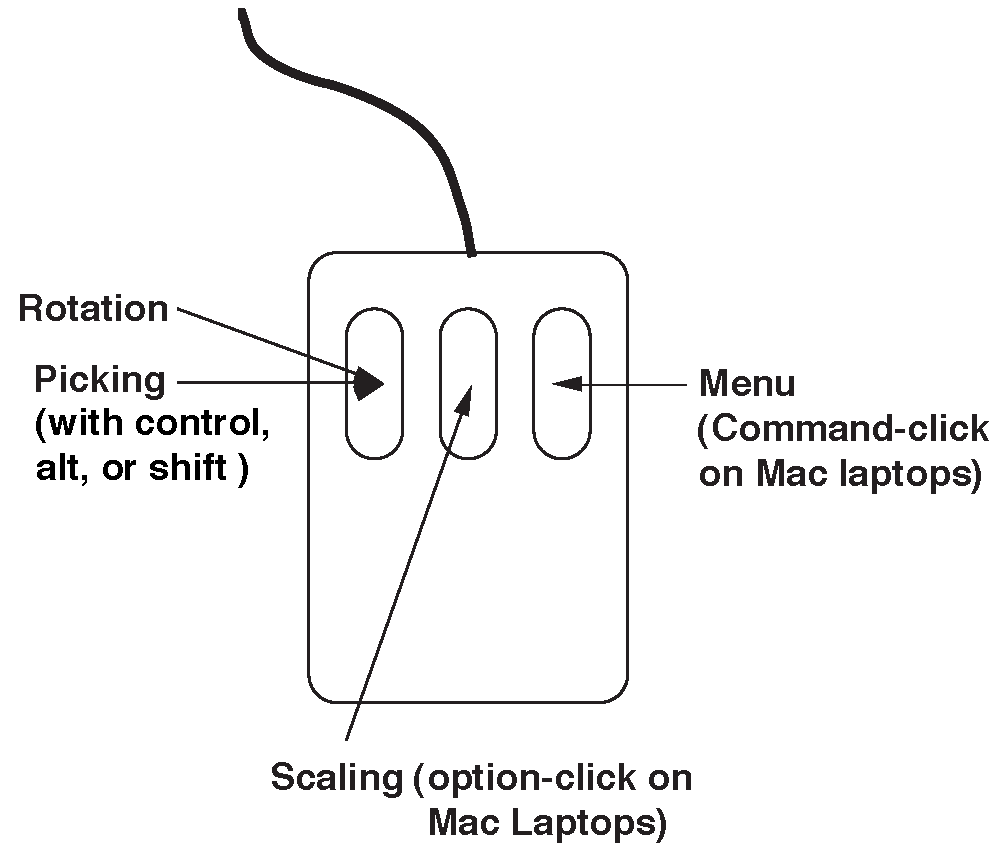
\includegraphics[height=2in]{figures/mouse.pdf}}}
  \newcommand{\filesdialogone}%
  {\centerline{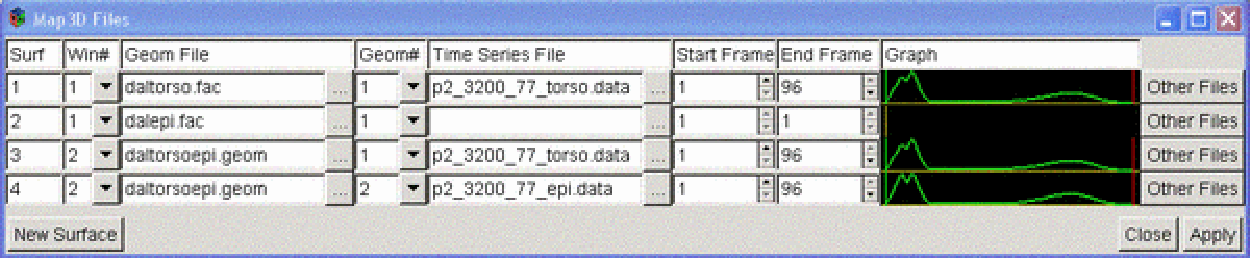
\includegraphics[width=\columnwidth]
      {figures/filesdialog1.pdf}}}
  \newcommand{\filesdialogthree}%
  {\centerline{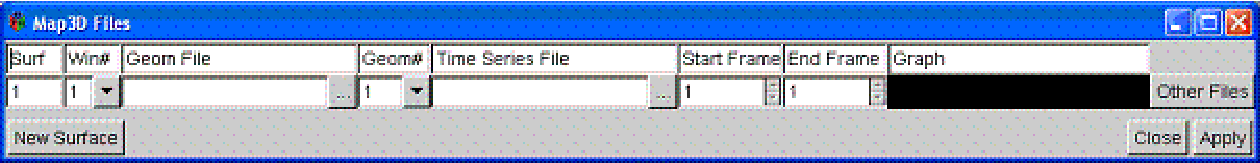
\includegraphics[width=\columnwidth]
      {figures/filesdialog3.pdf}}}
  \newcommand{\savedialog}%
  {\centerline{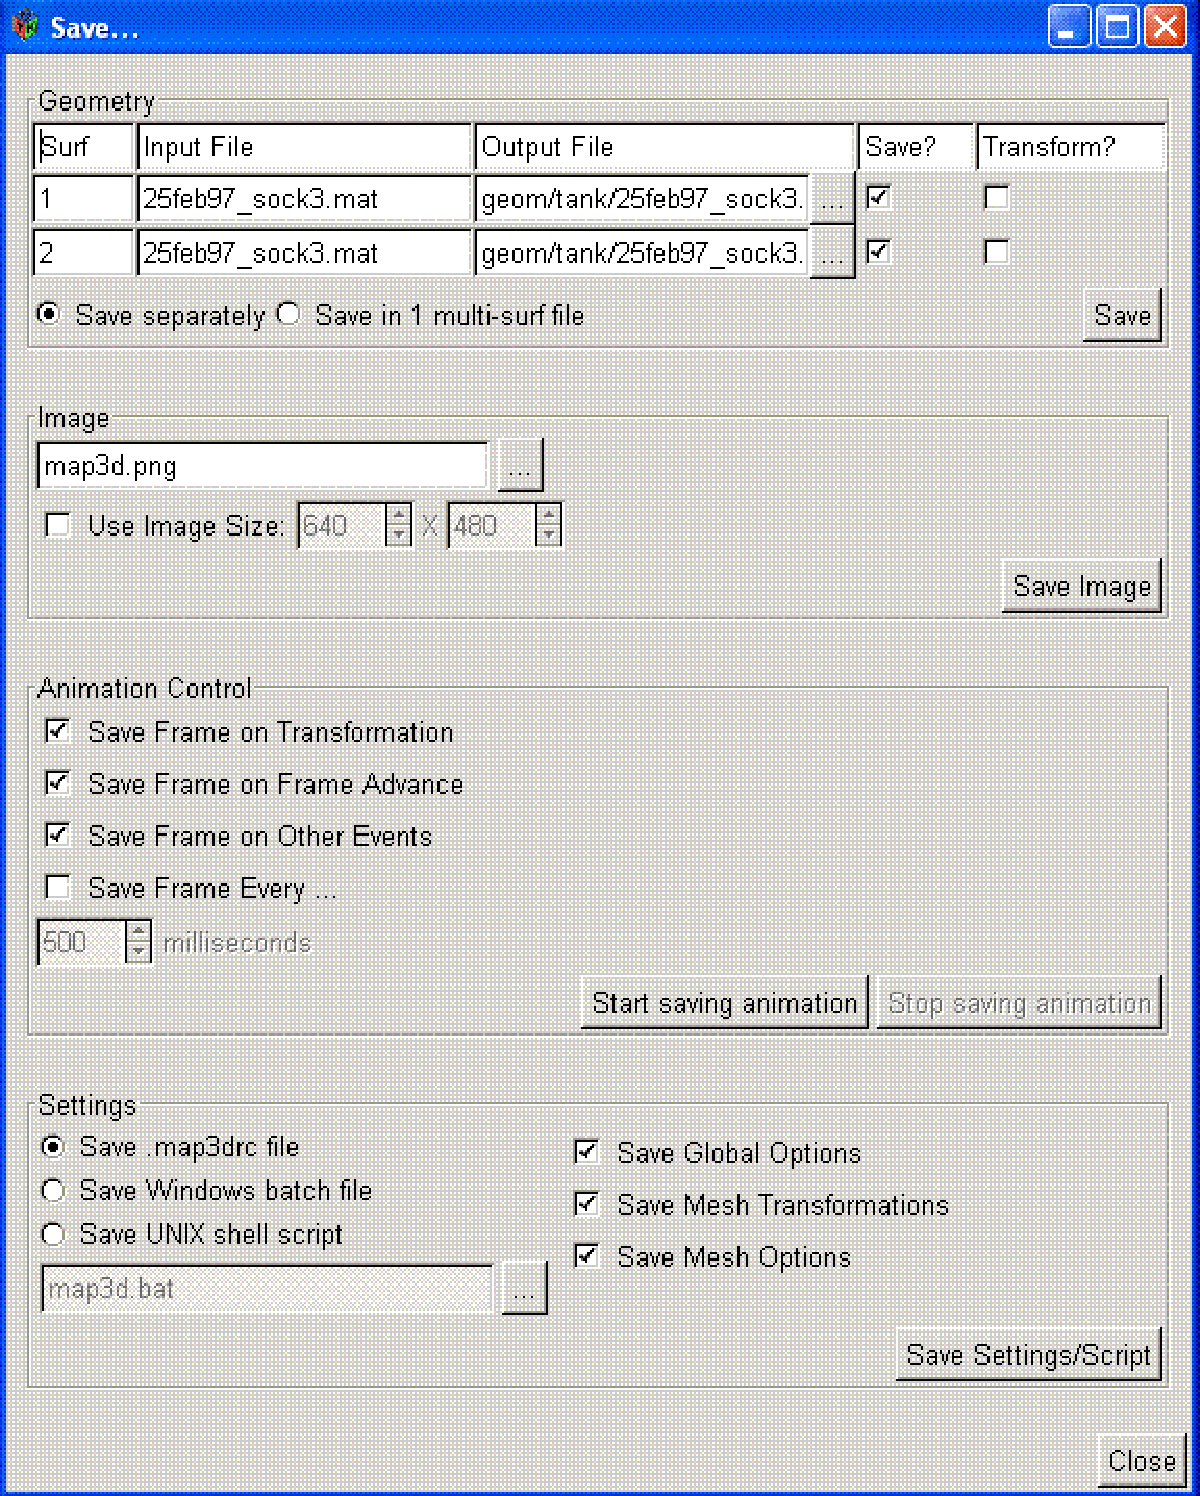
\includegraphics[height=4in]{figures/savedialog.pdf}}}
  \newcommand{\fiducialswindow}%
  {\centerline{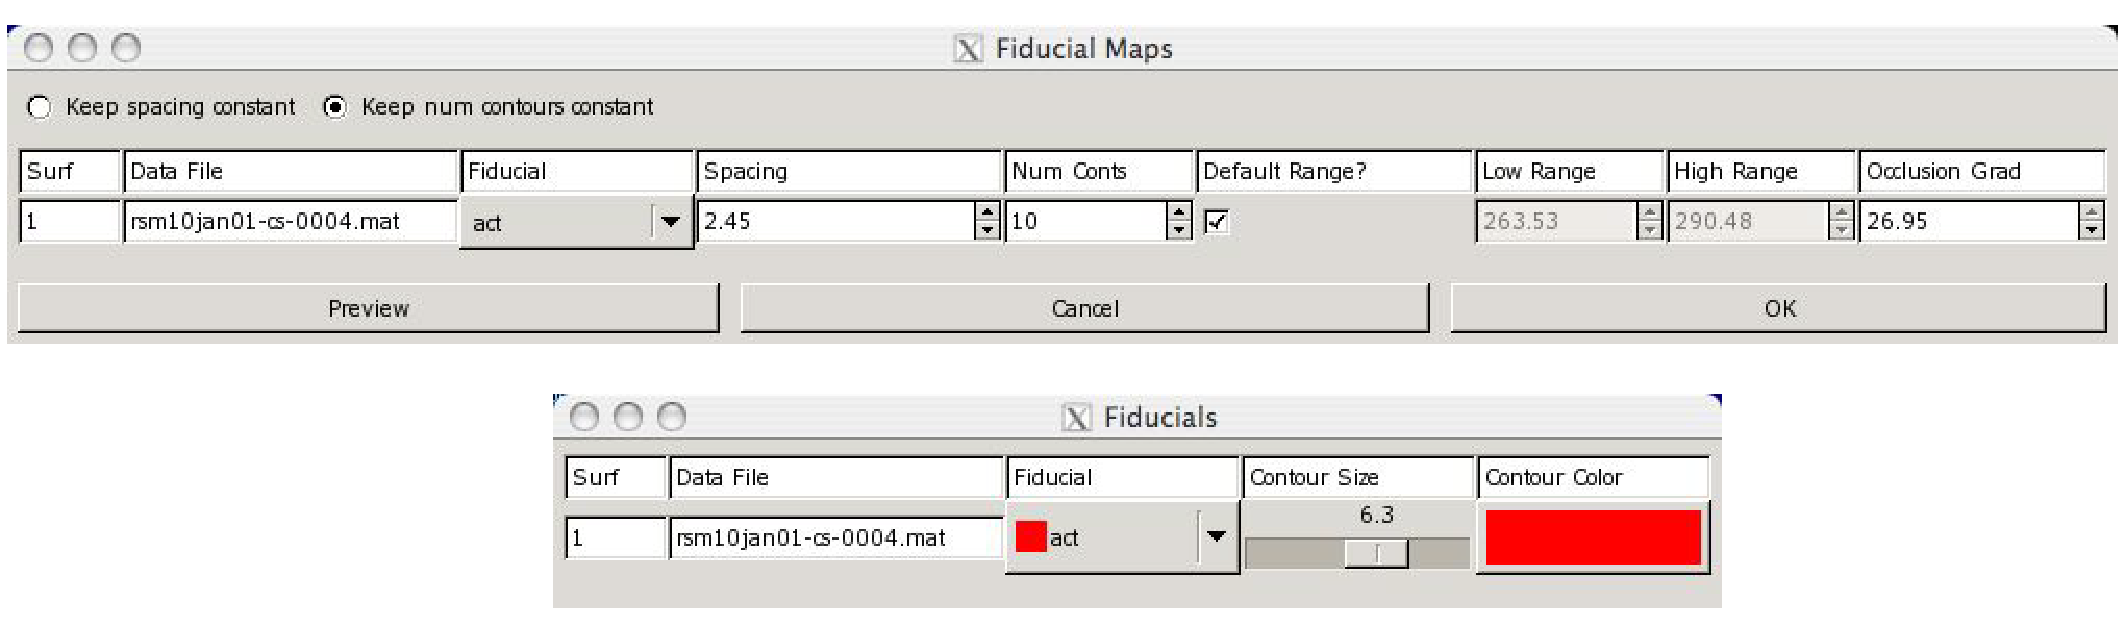
\includegraphics[width=\columnwidth]
  {figures/fidwindows.pdf}}} 
  \newcommand{\scaledialog}%
  {\centerline{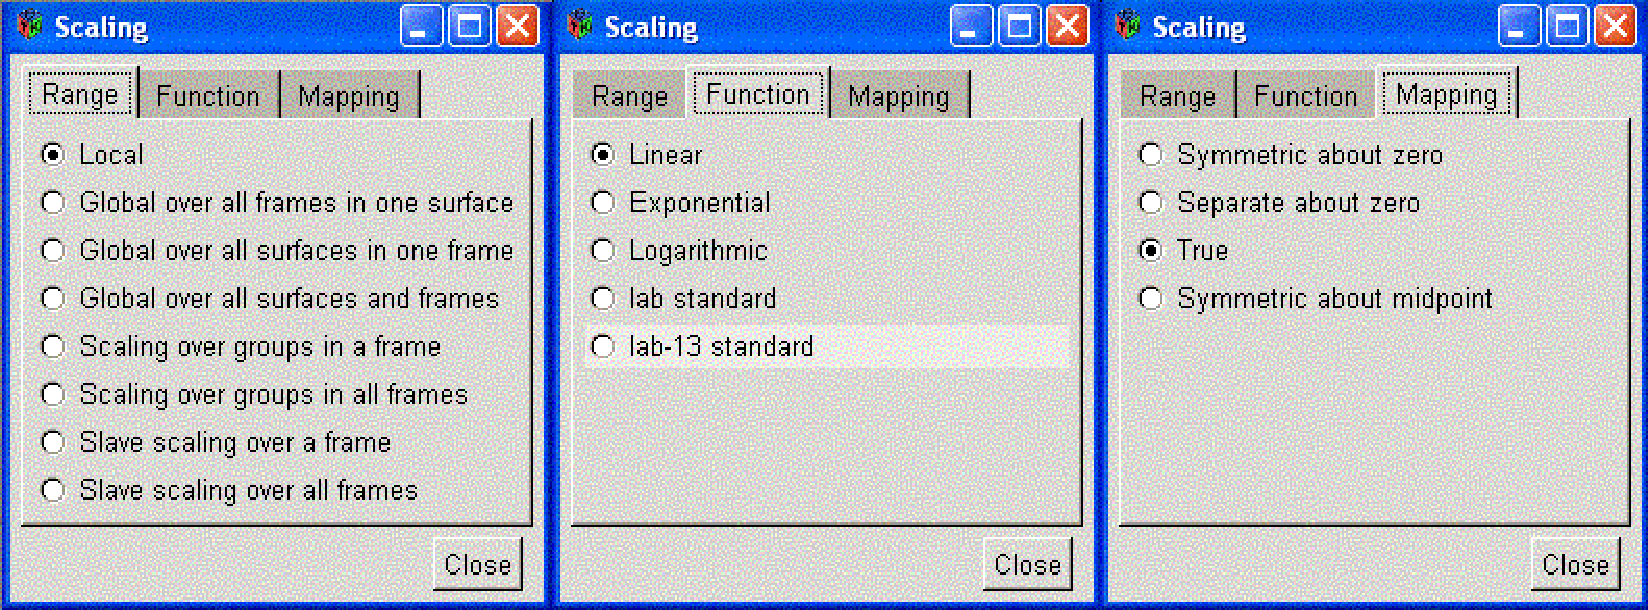
\includegraphics[height=2.5in]{figures/scaledialog.pdf}}}
  \newcommand{\contourdialog}%
  {\centerline{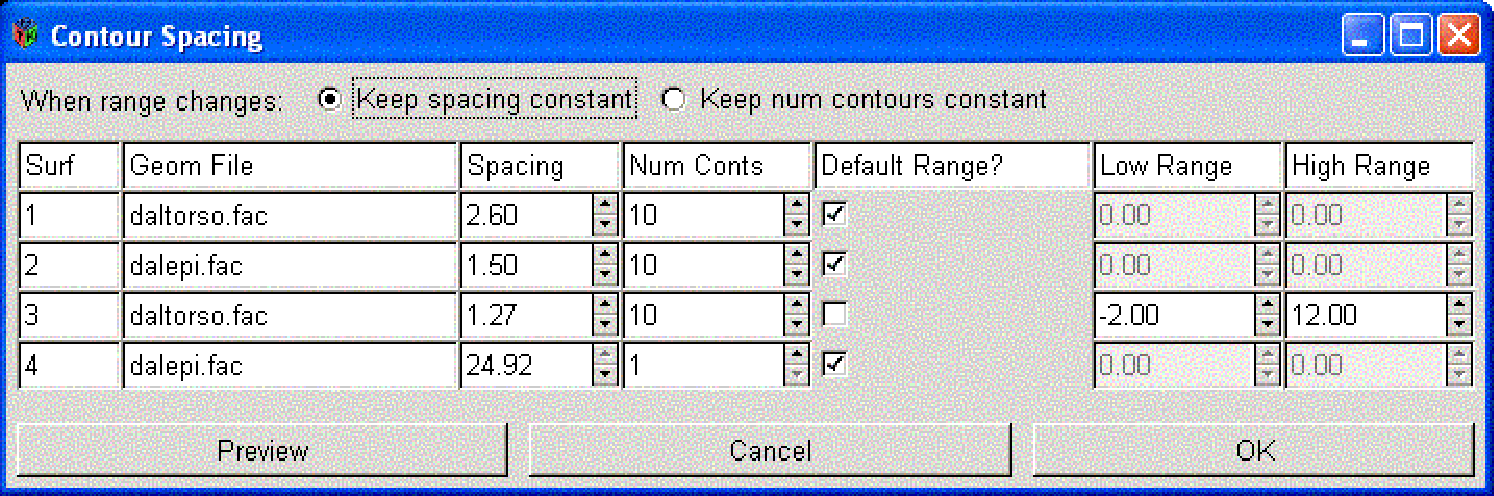
\includegraphics[height=2.5in]{figures/contourdialog.pdf}}}
  \newcommand{\colorpicker}%
  {\centerline{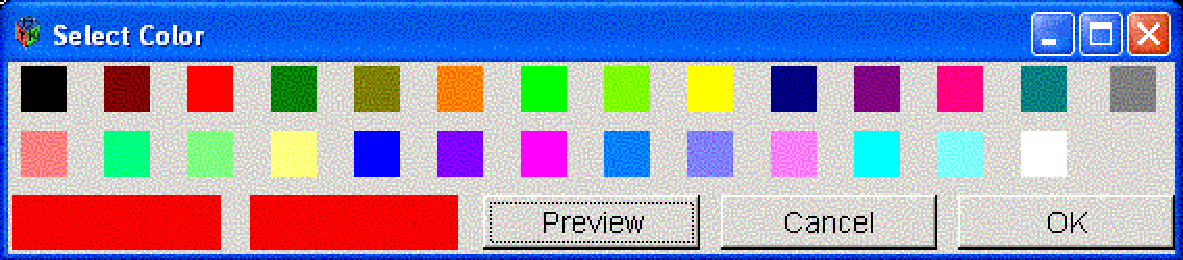
\includegraphics[height=1in]{figures/colorpicker.pdf}}}
  \newcommand{\sizepicker}%
  {\centerline{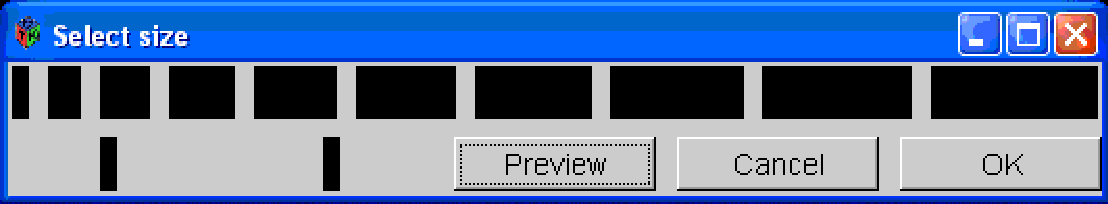
\includegraphics[height=1in]{figures/sizepicker.pdf}}}
%end{latexonly}
\begin{htmlonly}
  \newcommand{\mouseaction}{%
  \htmladdimg[align=top,width=371,alt="mouse action"]
  {../figures/mouse.jpg}}
  \newcommand{\filesdialogone}{%
  \htmladdimg[align=top,width=600,alt="Files Dialog"]
  {../figures/filesdialog1.gif}}
  \newcommand{\filesdialogthree}{%
  \htmladdimg[align=top,width=605,alt="Empty Files Dialog"]
  {../figures/filesdialog3.gif}}
  \newcommand{\savedialog}{%
  \htmladdimg[align=top,width=576,alt="Save Dialog"]
  {../figures/savedialog.gif}}
  \newcommand{\fiducialswindow}{%
  \htmladdimg[align=top,alt="Fiducials Window"]
  {../figures/fiduwindows.jpg}}
  \newcommand{\scaledialog}{%
  \htmladdimg[align=top,width=791,alt="Scaling Dialog"]
  {../figures/scaledialog.gif}}
  \newcommand{\contourdialog}{%
  \htmladdimg[align=top,width=717,alt="Contour Dialog"]
  {../figures/contourdialog.gif}}
  \newcommand{\colorpicker}{%
  \htmladdimg[align=top,width=568,alt="Color Picker"]
  {../figures/colorpicker.gif}}
  \newcommand{\sizepicker}{%
  \htmladdimg[align=top,width=532,alt="Size Picker"]
  {../figures/sizepicker.gif}}
\end{htmlonly}
%%%%%%%%%%%%%%%%%%%%%%%%%%%%%%%%%%%%%%%%%%%%%%%%%%%%%%%%%%%%%%%%%%%%%%
\newpage
\section{Control of \map{}}
\label{sec:control}

This section describes all the means of controlling the function of \map{},
at least all the ones we are willing to tell you about.


%%%%%%%%%%%%%%%%%%%%%%%%%%%%%%%%%%%%%%%%%%%%%%%%%%%%%%%%%%%%%%%%%%%%%%

\subsection{Control by surface}

There is an ever growing number of parameters that the user can alter
for displaying the surfaces in \map{}.  Some of the more important (and
stable) include the following:

\begin{description}
  \item [Visibility:] of points, mesh, potentials, vectors, \etc{} can all
        be controlled individually by using the appropriate function key
        (see Section~\ref{sec:control-keys}), 
      \item [Lead markings: ] of the nodes in the geometry according to
        their node number, channel number, lead number or even value,
  \item [Landmarks: ] appearance of the landmarks on the surface.
\end{description}

Since this level of control is provided for each surface, it is possible to
have points showing on one surface, mesh on another, and rendered potential
shading on a third, and so on. 

\subsubsection{Selecting which surface to control} 
\label{sec:locks} 

To control the display of each surface, be that a surface in its own window
or sharing a single window with other surfaces, a user must select that
surface.  Otherwise, display options will affect all the surfaces.  There
are two different multi-surface situations and each has its own method of
selecting the surface:
%
\begin{center}
  \begin{tabular}{|l|p{3in}|}\hline
    \multicolumn{2}{|c|}{Selecting surfaces for display controls} \\ \hline
    \multicolumn{1}{|c|}{Multi-surface layout} & 
    \multicolumn{1}{c|}{Selection method} \\ \hline
    One surface per window & Mouse location establishes currently active
    window. \\
    Several surfaces in one window & Up/down arrows selects the surface.
    Hitting 
    the up-arrow key after selecting the last surface selects all surface. \\
    \hline 
  \end{tabular}
\end{center}

Note that in the surface window, the lock icons in the lower left corner
indicate if parameter settings act on all surface (locks visible) or just
single surfaces (locks invisible).  Each lock controls a different aspect of 
\map{}:

\begin{description}
  \item [General Lock:] is represented by the yellow (or first) lock icon.  
        When this lock is active, menu items and keyboard commands pertain 
        to all surfaces.  To turn this lock off and on use the up
        and down arrow keys.
  \item [Transformation Lock: ] is represented by the red (or second) 
        lock icon.  When this lock is active, rotation and translation 
        pertain to all surfaces. To turn this lock on and off, use the
        ``t'' key.
  \item [Frame Lock: ] is represented by the blue (or third) lock icon.
        When this lock is active, frame advancing, retreating, and resetting
        pertain to all surfaces.  To turn this lock on and off, use the
        ``f'' key or select from the menu under \emph{Frame Controls}.
\end{description}

Note: in the case where all surfaces are in the same window, unlocking the
general lock by means of the up or down arrow keys selects the single
surface to display.  However, when the general lock is active and either of
the other locks is disabled, the active surface mesh appears in a different
color (blue by default).  This identifies the selected surface and all
modifications apply to this surface.  To select the desired surface use the
(/) keys; ``('' selects the next surface and ``)'' selects the previous.



%%%%%%%%%%%%%%%%%%%%%%%%%%%%%%%%%%%%%%%%%%%%%%%%%%%%%%%%%%%%%%%%%%%%%%

\subsection{Mouse control, keyboard mapping, dials, and menus}
 
Direct interactive control of \map{} is by the keyboard and mouse.
%mouse, and dials.
Many option are available via the menus controlled with the right mouse
button, while others can be activated or toggled with single keystrokes.
Variable (non-binary) adjustments usually occur 
% with the dials, if they are present, 
through dialogues, or by repeating keystrokes.  Below are tables of all the
current control devices and their function.  When the program launches, the
user sets one or more windows which can be resized and moved at any time.
When launching the program with the {\tt -b} option, the resulting
borderless sub-window(s) can still be moved and resized within a main
window using the Alt-key together with the left and middle mouse buttons
respectively.  In Mac OS X and other operating systems where the Alt-key is
mapped to another function you may use the CRTL+SHIFT keys as an
alternative to the Alt-key.


\subsubsection{Mouse control}
\label{sec:control-mouse} 

The mouse can be used for different purposes. Figure~\ref{fig:mouse} 
shows the various actions of the mouse
buttons. 

\begin{figure}[htb]
  \begin{makeimage}
  \end{makeimage}
  \mouseaction
  \caption{\label{fig:mouse} Mouse action for \map{}. Picking
  makes intensive use of the mouse, as does moving objects in the surface
  window.}
\end{figure}

\paragraph{In surface windows: } when the mouse is over a surface window,
mouse buttons have the following actions:
\begin{center}
  \begin{tabular}{|l|l|p{3in}|} \hline
    \multicolumn{3}{|c|}{Mouse Actions}\\ \hline
    \multicolumn{1}{|c|}{Control Key} & 
    \multicolumn{1}{|c|}{Button} & 
    \multicolumn{1}{|c|}{Action}\\ \hline
    None & Left & rotation objects \\
    & Middle & scale objects (downwards increases size, upwards decreases
    size) \\ 
    & Right & activate pull-down menu \\ \hline
    Cntrl & Left & pick a node (and if time series data is present, select the
    channel to display in the time series window) \\
    & Middle &  no action \\
    & Right &  no action \\ \hline
    Shift & Left & translate objects \\
    & Middle & scale objects (rotates clipping planes if they are active
    - more info later) \\ 
    & Right & no action \\ \hline
\end{tabular}
\end{center}

\paragraph{In borderless windows: } when the mouse is over a 
surface within a borderless main window (-b option), the buttons have the
following additional actions: 
\begin{center}
  \begin{tabular}{|l|l|p{3in}|} \hline
    \multicolumn{3}{|c|}{Mouse Actions}\\ \hline
    \multicolumn{1}{|c|}{Control Key} & 
    \multicolumn{1}{|c|}{Button} & 
    \multicolumn{1}{|c|}{Action}\\ \hline
    Alt(Ctrl+Shift)   & Left & Move a single surface subwindow \\ 
      & Middle & Resize single surface subwindow (no indication of change
    until release of mouse button).\\ 
      & Right & no action \\ \hline
  \end{tabular}
\end{center}

Note: if \map{} does not respond as described in these tables, it may be
that your window manager is grabbing the mouse/key combinations for its own
purpose or maps the keys a little differently.  This will require some
setting changes for the window manager.  In Linux there is usually a
control panel or utility application to manage all window system
interactions.

%\newpage

\subsubsection{Keyboard controls}
\label{sec:control-keys} 

Each key of the regular keyboard, the function keys, and the keypad may be
mapped to some function of the \map{}.  Some keyboard keys serve as toggles
to change between a mode being on or off, \eg{} ``n'' toggles the display
of node markings.  Others cycle through a set of choices, \eg{} ``m'' runs
through a series of display options for the mesh.  Several lists of the
keyboard keys and their functions are shown in
Tables~\ref{table:keys}--\ref{table:keypad}.

\begin{table}[htbp]
%\nopagebreak[4]
        \caption{\label{table:keys} Keyboard controls for Geometry Window
          in map{}.  When control contains both lower and upper cases of a
          letter, one cycles through a parameter in one direction and the
          other in the reverse direction.}
    \begin{center}
        \begin{tabular}{|l|p{6in}|} \hline
        \multicolumn{2}{|c|}{\textbf{Regular keyboard}} \\ \hline
        a/A-key   &       Switch colour tables \\ \hline
%        B-key  &       Toggle clipping plane \\ \hline
        c-key   &       Toggle contour draw \\ \hline
        d-key   &       Toggle depth cueing\\ \hline
%        E-key   &       Toggle backfacing visibility\\ \hline
        f-key   &       Toggle frame lock (also in Time signal window)\\ \hline
%        F-key   &       Shift focus to next window \\ \hline
       g-key   &       Toggle style of gouraud shading (between
       texture-mapped and non-texture-mapped) \\ \hline 
%       H-key   &       Set the location of the video box \\ \hline
        i-key   &       Toggle ``direction'' (invert) of color table\\ \hline
        l-key   &       Toggle use of lighting\\ \hline
        m/M-key   &       Step through mesh/node drawing options \\ \hline
        n-key   &       Toggle display of node labels (some node marking
        must be selected)\\ \hline 
%        O-key   &       Toggle ortho/perspective views \\ \hline
        p-key   &       Toggle information in time signal (pick) window
         (also in Time Signal Window)\\ \hline 
         q-key   &       Quit or destroy a sub-window - Legend Window and
         Time Signal Window only (Escape quits the 
                         whole program) \\ \hline
        r-key   &       Reset to startup conditions \\ \hline
        R-key   &       Reset shading model (to wireframe rendering) \\ \hline
%       S-key   &       Saves a .pts and a .fac file of the current 
%       geometry \\ \hline
        s/S-key   &      Cycle through the various surface data draw 
        options \\ \hline
        t-key   &       Toggle transformation lock \\ \hline
%        T-key   &       Whatever Rob is currently testing \\ \hline
%       U-key   &       Toggle locking of clipping planes \\ \hline
%       V-key   &       Toggle video mode \\ \hline
        w-key   &       Write an image to a file.  This will append a 4-digit 
                        number representing a image sequence number to the 
                        base filename (before the extension).  The base 
                        filename can be set at start-time with the -if flag 
                        (see Section~\ref{sec:usage-global}), or in the 
                        Save... Dialog (Section~\ref{sec:saving}).  \\ \hline
        x-key   &       Draw axis \\ \hline
%        Z-key   &       Rotate about z-axis in steps \\ \hline
        Escape  &       Quit the program, if pressed in a Geometry Window, 
            or Destroys a Time Signal Window if pressed there. \\ \hline
        +/- key   &    Increases/Decreases size of of currently-selected object
       (see Section~\ref{sec:interactive-size})\\ \hline
       ( \& ) keys   &  Change which susrface inside a window will be affected
            when the general lock is on but the transform or frame lock is off
            (see Section~\ref{sec:locks})\\ \hline
\end{tabular}
\end{center}

\end{table} 

\begin{table}[htbp]
%\nopagebreak[4]
        \caption{\label{table:clipping} Clipping plane controls}
    \begin{center}
        \begin{tabular}{|l|p{6in}|} \hline
        \multicolumn{2}{|c|}{Clipping Controls} \\ \hline
        \verb|<|-key    &       Toggle front clipping plane \\ \hline
        \verb|>|-key   &       Toggle rear clipping plane \\ \hline
        [ \& ] keys   &     Move front clipping plane in (initially) +z/-z
             direction respectively \\ \hline
        \{ \& \} keys   &   Move rear clipping plane in (initially) +z/-z
                  direction respectively \\ \hline
        ,-key   &  Lock/Unlock clipping plane rotation with object
                   rotation (when unlocked, shift-Middle-click rotates clipping
                   planes) \\ \hline
        .-key   &  Lock/Unlock clipping planes from each other.
                   When active, clipping planes move together \\ \hline
\end{tabular}
\end{center}

\end{table} 

\begin{table}[htbp]
    \caption{\label{table:arrowkeys} Control of \map{} via the arrow keys}
\begin{center}
    \begin{tabular}{|l|l|} \hline
        \multicolumn{2}{|c||}{\textbf{Arrow Keys}} \\ \hline
        Left Arrow Key  &       Retreat by current frame step (Also in Time
        Signal Window) \\ 
        Right Arrow Key &       Advance by current frame step (Also in Time
        Signal Window)\\ 
        Up Arrow key    &       Select next surface \\
        Down Arrow Key  &       Select previous surface \\ \hline
    \end{tabular}
\end{center}

\end{table}


  %\medskip
\begin{table}[htbp]
    \caption{\label{table:keypad}
      Keypad controls in \map{} - have NUM-Lock off for these to work
      properly.  Again, based on how you have your keys mapped, you might
      have to use the non-keypad keys, but something should work for you
      for each key.}
\begin{center}

\begin{tabular}{|l|p{3in}|} \hline
        \multicolumn{2}{|c||}{\textbf{Keypad Keys}} \\ \hline
   Ctrl-Keypad Left-arrow  &  Y-axis rotate, CW (left)  \\ \hline
   Ctrl-Keypad Right-arraow  &  Y-axis rotate, CCW (right)\\ \hline
   Ctrl-Keypad Up-arrow  &  X-axis rotate, CCW (down) \\ \hline
   Ctrl-Keypad Down-arrow  &  X-axis rotate, CW (up) \\ \hline
   Ctrl-Keypad Home  &  Z-axis rotate, CCW  \\ \hline
   Ctrl-Keypad PgUp  &  Z-axis rotate, CW  \\ \hline
   Ctrl-Keypad End  &  Zoom down  \\ \hline
   Ctrl-Keypad PgDn  &  Zoom up  \\ \hline
%        Keypad 0  &  Shift clip plane  & 
%        Keypad .  &  Shift clip plane  \\ \hline
    Alt(or CRTL+SHIFT)-Keypad Left-Arrow  &  -X-translation (left) \\ \hline 
    Alt(or CRTL+SHIFT)-Keypad Right-Arrow  &  +X-translation (right)\\ \hline
    Alt(or CRTL+SHIFT)-Keypad Down-Arrow  &  -Y-translation (down) \\ \hline
    Alt(or CRTL+SHIFT)-Keypad Up-Arrow  &  +Y-translation (up) \\ \hline
    Alt(or CRTL+SHIFT)-Keypad Home  &  -Z-translation (away) \\ \hline
    Alt(or CRTL+SHIFT)-Keypad PgUp  &  +Z-translation (towards)  \\ \hline
        Plus/Minus key  & Increase/Decrease size of
    currently-selected object. (see Section~\ref{sec:interactive-size})\\
\hline
\end{tabular}
\end{center}
\end{table}
\clearpage


\subsubsection{Menu layout}
\label{sec:control-menus}

Access to the menus is by means of the right mouse button, as per the usual
OpenGL convention.  Below is a series of tables of the menu layout for
\map{}'s Geometry Window.

\begin{table}[ht]
\caption{\label{table:menu-geom}
  The overall menu structure in the Geometry Window}.
  \begin{center}
    \begin{tabular}{|l|p{4in}|} \hline
      \multicolumn{2}{|c|}{\textbf{Overview of Geometry Window menus}} \\
      \hline \hline 
      Files & Opens the Files Window (see Section~\ref{sec:fileswindow}) \\
      Save & Opens the Save Window (see Section~\ref{sec:saving})  \\
      Contours & number or spacing and display features of the contours \\
      Fiducials & Fiducial display features - Currently only opens the fiducial
        dialog.  (See Section~\ref{sec:fiducialswindow})\\
      Frame Controls & modifying frame controls\\
      Graphics & general display features such as lighting, clipping,
        and depth cueing \\
      Landmarks & features for toggling and displaying landmarks \\ 
      Mesh & display features of the mesh \\
      Node marking & marking of the nodes \\
      Picking & selecting times signals, mesh information, or other direct
      interactions with the display via the mouse\\
      Scaling & links between data values and color\\
      Surface Data & display features of the scalar data displayed on the
      mesh \\  
      Use +/- to select & Select a feature to change interactively with + or -
      \\
      Window Attributes & features of the windows such as color and text
      labels \\ \hline
    \end{tabular}
  \end{center}
\end{table}


\begin{table}[ht]
\caption{\label{table:contours}Menus for contour spacing/number.}
  \begin{center}
    \begin{tabular}{|l|l|p{3 in}|} \hline
      \multicolumn{3}{|c|}{\textbf{Contour Menus}} \\ \hline
    Set Contour Num/Spacing & & Opens a dialog to change user-specified 
    spacing or number of contours. See Section~\ref{sec:contourwindow}.
    \\ 
    Draw style & & \\
    & Dashed line for negative values & draw positive contours in solid,
    negative in broken lines\\
    & Solid lines for all contours & draw all contours in solid lines\\
    Line size & & set the line thickness \\ \hline
    Toggle contours & & toggle display of contours
    without changing settings \\ \hline
    \end{tabular}
  \end{center}
\end{table}

\begin{table}[ht]
\caption{Frame Controls.}
  \begin{center}
    \begin{tabular}{|l|l|p{2.8 in}|} \hline
      \multicolumn{3}{|c|}{\textbf{Frame Control Menus}} \\ \hline
    Lock Frames  & & toggle whether frames 
        operations affect one surface or all surfaces \\ \hline
    Set Frame Interval & & \\
      & Set Frame Step & Opens a dialog to interactively set User-specified 
    frame step.  Affected surfaces are determined by the lock status.\\
      & User-specified Interval & use the value of interval specified in the 
        \texttt{-i} option of the command line or the value set in the
        frame step dialog.\\ 
      & \emph{value} & select between 1 and 90 for frame animation step \\
    Reset Frames to 0 & & positions the surface at the first position in time
       \\
    Align meshes to this frame num & & Positions all surfaces' frames to the
    current surface.  What 'current surface' means will vary based on the status
    of the locks (see Section~\ref{sec:locks})
    \\
    Set time to zero & & Set current frame to be time zero.
        \\ \hline
    \end{tabular}
  \end{center}
\end{table}

\begin{table}[ht]
\caption{Graphics menus.  These control general graphic rendering options.}
  \begin{center}
    \begin{tabular}{|l|l|p{3 in}|} \hline
      \multicolumn{3}{|c|}{\textbf{Graphics Menus}} \\ \hline
    Light source & & select the source for the lighting model\\
    & From above &  \\
    & From below &  \\
    & From left &  \\
    & From right &  \\
    & From front &  \\
    & From back &  \\
    & None & no lighting (turn lighting off) \\ \hline
    Toggle clipping & & toggles particular clipping plane options \\
    & Front plane & toggles front clipping plane \\
    & Back plane & toggles rear clipping plane \\
    & Locking planes together & makes planes translate together\\
    & Locking planes with object & rotate surface with the planes or
        rotate surface through the planes \\
    Toggle Depth cue & & apply/disable depth cueing (fog) \\
    Adjust Depth cue & & Opens a dialog to adjust the front and rear planes
    to where the depth cueing occurs. \\
    \hline
    \end{tabular}
  \end{center}
\end{table}

\begin{table}[ht]
\caption{Submenus for the Mesh Display menu}
  \begin{center}
    \begin{tabular}{|p{1in}|p{2in}|p{2.5in}|} \hline
      \multicolumn{3}{|c|}{\textbf{Mesh render menu}} \\ \hline
    Render as & & \\
      &  None & Do not render the mesh \\
      &  Elements  & render filled surfaces for all elements \\
      &  Connectivity & render connectivity mesh\\ 
      &  Elements and connectivity & rendered front facing triangles as
            elements and back facing as connectivity \\ 
      &  Points & render points \\ 
      &  Points and connectivity & render both points and connectivity \\ 
      \hline
    Line/point size 
      & \multicolumn{2}{|l|}{set the size of the mesh's points and lines}\\
    \hline 
    Color 
      & \multicolumn{2}{|l|}{set the color of the mesh}\\ \hline
    Secondary Mesh Color
      & \multicolumn{2}{|l|}{set color of active mesh when multiple 
        surfaces are in same window} \\ \hline
    Show Legend Window
      & \multicolumn{2}{|l|}{display mesh's legend window}\\ \hline
    Hide Legend Window
      & \multicolumn{2}{|l|}{turn off display of mesh's legend window}\\ \hline
    Reload Geometry
      & \multicolumn{2}{|l|}{reload file associated with this geometry}\\
    \hline 
    Reload Surface Data
      & \multicolumn{2}{|l|}{reload file associated with this geometry's
    surface data}\\ \hline 
    Reload Both Geometry and Data
      & \multicolumn{2}{|l|}{reload files associated with this geometry and
    its data}\\ \hline 

    \end{tabular}
  \end{center}
\end{table}

\begin{table}[ht]
    \caption{\label{table:nodemarking} Menus for marking nodes in the display.
      If all surfaces are currently displayed, any of these settings will affect
      all surfaces based on the rules in locks section (see
      Section~\ref{sec:interactive-size}).  If we have a single  
      or current) surface only, then change only that surface.}
  \begin{center}
    \begin{tabular}{|l|l|p{4 in}|} \hline
      \multicolumn{3}{|c|}{\textbf{Node Marking Menus}} \\ \hline
    All & & Make all the nodes in this (or all) surface(s) \\
    &  Sphere & mark each node with a sphere \\
    &  Map data to spheres & mark each node with a sphere, whose
                             color reflects its scalar data value \\
    &  Node \# & mark each node with the node number in the geometry \\
    &  Channel \# & mark each node with the associated data channel number \\
    &  Data value & mark each node with the associated data value \\
    &  Color & set the color for marking all nodes \\
    &  Size & set the size of all node markings \\
    &  Clear all marks & remove all node marking settings \\ 
    \hline
    Extrema & & Make all the nodes that are the extrema  \\
    &  Sphere & mark each extrema with a sphere \\
    &  Node \# & mark each extrema with the node number in the geometry \\
    &  Channel \# & mark each extrema with the associated data channel
    number \\ 
    &  Data value & mark each extrema with the associated data value \\
    &  Size & set the size of all extrema markings \\
%    &  Color & set the color for marking all extrema \\
    &  Clear all marks & remove all extrema marking settings \\ 
    \hline
    Time signal & & Make all the nodes that identify the location of time
    signals shown in the display  \\
    &  Sphere & mark each times signal location with a sphere \\
    &  Node \# & mark each times signal location with the node number in
    the geometry \\ 
    &  Channel \# & mark each times signal location with the associated
    data channel number \\ 
    &  Data value & mark each times signal location with the associated
    data value \\ 
    &  Color & set the color for marking all times signal locations \\
    &  Size & set the size of all time signal markings \\
   &  Clear all marks & remove all time signal marking settings \\ 
    \hline
    Lead links & & Make all the nodes that identify the features from
    leadlinks file 
       (see Section~\ref{sec:leadfiles}) shown in the display  \\
    &  Sphere & mark each lead location with a sphere \\
    &  Node \# & mark each lead location with the node number in
    the geometry \\ 
    &  Channel \# & mark each lead location with the associated
    data channel number \\ 
    &  Data value & mark each lead location with the associated
    data value \\ 
    &  Lead labels & mark each lead with the label from the leadlinks file.\\
    &  Color & set the color for marking all lead locations \\
    &  Size & set the size of all lead markings \\
   &  Clear all marks & remove all lead marking settings \\ 
    \hline
    \end{tabular}
  \end{center}
\end{table}

\begin{table}[ht]
    \caption{\label{table:pickingone} Pick mode menus, part 1.  Picking is
      based on a 
      mode (selectable in this menu), and is done with CTRL-left mouse button
      unless otherwise specified.}
  \begin{center}
    \begin{tabular}{|l|p{4 in}|} \hline
      \multicolumn{2}{|c|}{\textbf{Picking Menus I}} \\ \hline
      Time Signal (new window mode) & create a new time signal window with
      each pick of a node \\
      Time Signal (refresh window mode) & update the last time signal 
      window with each pick of a node \\
      Display node info mode & Picking will cause certain node information
      to be dumped to the console. \\
      Display triangle info mode & Picking will cause information about
      the triangle you click in to be dumped to the console.
      It may be easier to pick triangles with clipping planes on. \\
      Triangle construction/deletion & Normal picking (ctrl-clicking on nodes)
      will select points to form a triangle (triangulate).  Clicking the first 
      two nodes in this fashion will display the selected nodes, and then a 
      line between the two.  When the third is clicked, a new triangle is 
      displayed and added to the geometry. \\
      & CTRL-middle clicking selects a triangle (and not nodes) to be deleted.
      Again, it may be easier to pick triangles with clipping planes on. \\
      Flip triangle mode & Will change the order of drawing the triangle's
      points.  This will cause front-facing triangles to become back-facing
      and vice-versa. \\
      Edit node mode & Will allow you to pick a point and translate it
      with the keyboard transform controls (see
      Section~\ref{sec:control-keys}, keypad controls) \\
      Edit landmark point mode & Will allow you to pick a landmark point
      and translate it with the keyboard transform controls (see
      Section~\ref{sec:control-keys}, keypad controls) \\
      Delete node mode & Will remove from the geometry any node that you pick
      and any triangles associated with it. \\
      \hline
  \end{tabular}
\end{center}
\end{table}

\begin{table}[ht]
  \caption{\label{table:pickingtwo} Pick mode menus, part 2.  Picking is
    based on a 
    mode (selectable in this menu), and is done with CTRL-left mouse button
    unless otherwise specified.}
  \begin{center}
    \begin{tabular}{|l|p{4 in}|} \hline
      \multicolumn{2}{|c|}{\textbf{Picking Menus II}} \\ \hline
    Reference lead, single value & Causes all values to be measured
    against the node which you pick \\
    Reference lead, mean value & Causes all values to be measured
    against a mean value of all the nodes \\
    Reset Reference & Causes the reference and values to be reset to
    its original value.  You must reset the reference if you want to
    change the reference more than once. \\
    Show Time Signal Window info & Toggles display modes in time series window.
    When there is no info, the graph takes up more room in the window. 
    This is equivalent to pressing 'p' in a geometry window or selecting
    the toggle display mode option of a time series window's menu. \\
    Show all pick windows & Causes all Time Series (Pick) Windows
    associated with this geometry to become visible. \\
    Hide all pick windows & Causes all Time Series (Pick) Windows
    associated with this geometry to become hidden. \\ 
    Size of picking aperture & select the size of the region around the
    mouse 
    pointer that will register a ``hit'' when picking; larger values will
    make it easier to pick an object but also easier to hit multiple
    objects. \\ 
    Size of triangulation node mark & when triangulating, a node
    mark will appear on the node(s) selected.  Adjust that mark's size. 
    \\ \hline
    \end{tabular} 
  \end{center}
\end{table}

\begin{table}[ht]
    \caption{Menu for scaling, the mapping from data value to color for
      rendering. }
\label{table:scaling}
  \begin{center}
    \begin{tabular}{|l|l|p{3 in}|} \hline
      \multicolumn{3}{|c|}{\textbf{Scaling Menus}} \\ \hline
    Scaling... & \multicolumn{2}{|l|}{opens up the scaling dialog.  (see
    Section~\ref{sec:scalinggui})} \\
    Range & & \\
    &  Local  & scale based on the local extrema for each surface and time
       instant \\
    &  Global over all frames in one surface  & scale based on the extrema 
        over the full times series \\ 
    &  Global over all surfaces in one frame & scale based on the extrema over 
        each surface for the local time instant\\
    &  Global over all surfaces and frames & scale based on the extrema
    over all surfaces 
       and all time instants\\
    &  Scaling over groups in one frame & scale based on the extrema over 
        each surface in specified group for the local time instant\\
    &  Scaling over groups in all frames & scale based on the extrema over 
        each surface in a specified group for all time instants\\
    &  Slave Scaling over one frame & scale based on the extrema over 
        each surface's master surface (set with -sl in command line)
        for one time instant\\
    &  Slave Scaling over all frames & scale based on the extrema over 
        each surface's master surface (set with -sl in command line)
        for all time instants\\ \hline

    Function & & \\
    &  Linear & linear mapping between value and color \\ 
    &  Logarithmic & color changes as  $\log({\rm value})$ \\ 
    &  Exponential & color changes as  $\exp({\rm value})$ \\ 
    &  Lab standard & color reflects lab standard \\ 
    &  Lab 13 standard & color reflects lab 13 standard \\ \hline
    Mapping & & \\ 
    &  True & use true extrema \\ 
    &  Symmetric about zero & take largest of absolute values of extrema to
    determine scaling \\
    &  Symmetric about midpoint & scale independently on both sides of the
    midpoint to determine scaling \\
    &  Separate about zero & scale positive and negative portions of the
    scale independently \\ \hline
    Grouping & & \\
    &  Move to group \# & Select a group to place the current surface
    (make sure the general (yellow) lock is off, or all surfaces
    will be placed in that group) \\ \hline
    \end{tabular}
  \end{center}
\end{table}

\begin{table}[ht]
    \caption{Submenus to control the display of scalar data on the mesh.}
  \begin{center}
    \begin{tabular}{|l|l|p{2.5 in}|} \hline
      \multicolumn{3}{|c|}{\textbf{Surface Display Menus}} \\ \hline \hline
    Color & & \\
    &  Rainbow  & use rainbow color map to render scalar values on the mesh\\
    &  Green to red & use green to red color map\\
    &  White to Black & use black and white color map\\ 
    &  Invert & invert the sense of any color map, \eg{} black becomes
        white and white becomes black \\ \hline
    Render style & & \\
    &  None & Turn Shading off \\
    &  Flat & colour each mesh element in a constant
       color according to the mean value of scalar data over the vertices\\
    &  Gouraud & shade each polygon using linear interpolation \\
    &  Banded & draw the regions between contour lines as bands of constant
       color\\  \hline
    \end{tabular}
  \end{center}
\end{table}

\begin{table}[ht]
    \caption{The Use +/- to interactively change sizes menu}
  \begin{center}
    \begin{tabular}{|l|p{4in}|} \hline
      \multicolumn{2}{|c|}{\textbf{+/-  Adjust Menu.}} \\ \hline \hline
      Large Font Size & Change the largest font size (This is the title
    for the Colormap and Geometry windows) \\ 
      Medium Font Size & Change the medium font size (This is all text
    not small or large) \\ 
      Small Font Size & Change the small font size (This is the size for
    the node marks, the axis labels in the Time Signal Window, and the
    Contour Labels in the ColorMap Window) \\ 
      Contour Size & Change the contour width \\
      Line/Point Size & Change the width of Lines/Points in the mesh \\
      Node Marks (all) Size & Change the width of node marks \\
      Node Marks (extrema) Size & \\
      Node Marks (time signal) Size & \\
      Node Marks (leads) Size & \\
      Change in translation & Change how fast the keyboard translation
    happens \\ 
      Change in scaling & Change how fast the keyboard scaling happens \\
      Change in rotation & Change how fast the keyboard rotation happens
      \\ \hline 
    \end{tabular}
  \end{center}
\end{table}



\begin{table}[ht]
  \caption{Controls for the attributes of the \map{} windows.}
  \begin{center}
    \begin{tabular}{|l|l|p{3 in}|} \hline
      \multicolumn{3}{|c|}{\textbf{Window Attributes Menus}} \\ \hline
    Screen info & & select the text written to the screen.  
    Note that screen info 
       disappears when clipping is on.\\
      & Turn screen info on & \\
      & Turn screen info off & \\ 
      & show/hide lock icons & toggle lock display \\ \hline
      & Show Legend Window & Turns on Colormap window \\ 
      & Hide Legend Window & Turns off Colormap window \\ 
    Color & & select window colors with the separate color selector \\
      & Background & select background color for the window \\
      & Foreground & select foreground color for the window \\ \hline
    Size & & select some size options \\
      & \emph{value} & set window to specified resolution \\
    Axes & & select options for axes \\
      & Axes Color & Select axes color \\
      & Axes Placement & select whether axes displayed per window or mesh \\
      & Toggle Axes & turn on/off axes \\ \hline
    Font Size & & Use the Size Picker to adjust the font size \\
      & Small Font Size & Size of node mark text or Colormap window contour 
        ticks \\
      & Medium Font Size & Size of window subtitles or text in Pick Window \\
      & Large Font Size & Size of Window titles \\
    Toggle Transformation Lock & & toggle whether surfaces transform 
        together or independently \\ \hline
    \end{tabular}
  \end{center}
\end{table}


\begin{table}[ht]
\caption{Controls for the attributes of the Time Signal Window.}
  \begin{center}
    \begin{tabular}{|l|p{4in}|} \hline
      \multicolumn{2}{|c|}{\textbf{Time Signal Window Controls}}
      \\ \hline \hline
      Axes Color & Select Axes Color \\
      Graph Color & Color of data graph \\  
      Toggle Display Mode & Show basic values and graph, show
      detailed values and graph, or show larger
      graph\\ \hline
    \end{tabular}
  \end{center}
\end{table}


\begin{table}[ht]
\caption{Controls for the attributes of the Legend window.}
  \begin{center}
    \begin{tabular}{|l|l|p{3 in}|} \hline
      \multicolumn{3}{|c|}{\textbf{Legend Window Controls}} \\ \hline
    Orientation & & Layout of information in Legend Window\\
      & Vertical & \\
      & Horizontal & \\ \hline
    Number of Tick Marks & & select number of ticks to appear on bar \\
      & 2,4,8 & Either 2,4,8 ticks.  These will not be colored as they do not
        directly correspond to contour values. \\
      & Match Contours & Match number of contours in corresponding geometry
    \\ \hline 
    \end{tabular}
  \end{center}
\end{table}

\begin{table}[ht]
\caption{Controls for the Legend Window Menu}.
  \begin{center}
    \begin{tabular}{|l|p{4in}|} \hline
      \multicolumn{2}{|c|}{\textbf{Main Window Controls}} \\ \hline \hline
      Set Background Color & Select bg Color \\
      Quit Map3D & Quit Map3D \\ \hline
    \end{tabular}
  \end{center}
\end{table}

\clearpage


%  Report level & & \\
%     & \multicolumn{2}{l|}{Level 0 = default} \\
%     & \multicolumn{2}{l|}{Level 1 = report extrema} \\
%     & \multicolumn{2}{l|}{Level 2 = mild debugging}  \\
%     & \multicolumn{2}{l|}{Level 3 = moderate debugging} \\
%     & \multicolumn{2}{l|}{Level 4 = max debugging} \\ \hline
%  \hline
%Save settings & & \\
%   & \multicolumn{2}{l|}{save in local .map3drc} \\
%   & \multicolumn{2}{l|}{save in home .map3drc} \\ \hline

%%%%%%%%%%%%%%%%%%%%%%%%%%%%%%%%%%%%%%%%%%%%%%%%%%%%%%%%%%%%%%%%%%%%%%

%  \subsection{Feedback Reporting Level}

%  In order to control the amount of printed feedback \map{} provides (which
%  is posted in the window from which the program was launched), the user can
%  select a value between 0 and 3 from the a sub-menu of the main menu titled
%  {\em Report level}.  The settings and level of output are as follows:


%  \begin{center}
%  \begin{tabular}{|c|l|} \hline
%    \multicolumn{1}{|c|}{Report Level} &
%    \multicolumn{1}{|c|}{Types of output} \\ \hline
%    0 & minimal output --- just changes in status \\
%    1 & report extrema \\
%    2 & report some warning messages \\
%    3 & debug mode \\ \hline
%  \end{tabular}
%  \end{center}


%%%%%%%%%%%%%%%%%%%%%%%%%%%%%%%%%%%%%%%%%%%%%%%%%%%%%%%%%%%%%%%%%%%%

\subsection{Interactive GUIs - File Selection, File Saving, and Scaling
  Options, \etc{}} 
\label{sec:interactive}

With the move to a deidcated GUI system (in our case, gtk), we make use of
a number of different windows to select parameters and control \map{}.
This section covers the functionality of all of them.

\subsubsection{Files Window}
\label{sec:fileswindow}

\begin{figure}[htb]
  \begin{makeimage}
  \end{makeimage}
  \filesdialogone
  \caption{\label{fig:file1} Files Dialog for \map{}.}
\end{figure}

The most frequently used GUI window is the ``\map{} Files'' window, allows
you to interactively select filenames, data windows, etc.  The others are
for saving files, and for quick scaling changes.  Figure~\ref{fig:file1}
shows an example of such a file window, and access to this window is by
means of the ``Files'' menu option of the main menu.  This window displays
one row for each surface, where each row shows the surface number, the
window the surface appears in, the geometry filename, the geometry number,
the data filename, the start frame number, the end frame number, a graph of
the RMS curve, and a button to show other files.  Most of these columns can
be modified at any time.  If you click on the ``New Surface'' button, an
empty row will pop up, allowing you to add a surface from scratch.
 
None of the changes made to this window will take effect until you click on
the ``Apply'' button.  The  ``Close'' button will cause  the window
will close, but opening it again will reveal the same content.

\begin{table}[htbp]
\caption{\label{table:filewindow} Options for the file window}    
\begin{center}
\begin{tabular}{|l|p{4in}|} \hline
    \multicolumn{2}{|c|}{\textbf{File Window Options}} \\ \hline\hline
    Surf      &      Number of the surface \\ \hline
    Win\#      &      Number of the window that contains this surface.
          You can change this number to move the surface to any
          open window, or to a new window (by selecting the last
          number from the drop-down menu). \\ \hline
    Geom File &      Name of the geometry file of this surface.  To change
        the geom file click on the
        ... button and then browsing for the desired file. You may reload the
        current geometry by  
        selecting the ``Mesh$\Rightarrow$Reload Geometry'' 
        menu entry. \\ \hline
    Geom\#     &      Number of surface within the geometry file (see
         Section~\ref{sec:geomfile}). 
         If there is more than one surface in the geometry
         file, an associated drop-down  menu selects which one to 
         insert.   \\ \hline
    Time Series File      &   Name of the data file of this surface.
         As with geometry  clicking on the ... button launches 
         a file browser to select a time-series data file.
         Selecting the ``Mesh$\Rightarrow$Reload Data'' reloads
         the data. \\ \hline
    Start Frame           &   Start reading data at this frame. 
         Left-clicking 
         in the graph section and dragging will also  select the
         correct frame. \\ \hline
    End Frame             &       Finish reading data at this frame.
         Middle-clicking in the graph section and draging 
         will  select the correct frame. \\ \hline 
    Graph     &       Graph of the root-mean-square signal calculated
         from all signals in the time series.    Left- or
         middle-clicking in this graph selects the data window that
         \map{} will read and display. \\ \hline 
    Other Files           &       This button will pop open another
         window in which to view/modify the channels, leadlinks, 
         landmarks, or fiducial file to use with this surface. \\ \hline 
\end{tabular}
\end{center}
\end{table}


\begin{figure}[htb]
  \begin{makeimage}
  \end{makeimage}
  \filesdialogthree
  \caption{\label{fig:file3} Empty Files Dialog. \map{} will start up this way
            if launched without arguments.}
\end{figure}

Note that the File window allows launching of \map{} without any arguments.
In this case an empty file window appears, as in Figure~\ref{fig:file3} so
that the user can select all the files for display and set up the display
interactively.


\subsubsection{Saving Files}
\label{sec:saving}

\begin{figure}[htb]
  \begin{makeimage}
  \end{makeimage}
  \savedialog
  \caption{\label{fig:save1} Saving Dialog.}
\end{figure}


The ``Save...'' Window will appear if after selecting ``Window
Attributes$\Rightarrow$Save...''  from the main \map{} menu.  The first
section is for saving geometry files, the second is for images, and the third
for settings.

\paragraph{Saving Geometry}
\label{sec:savegeom}

The Geometry section displays each surface number with its current geometry
filename and next to each is a check box.  If that check box is checked
when the user clicks one of the save buttons, then that surface will be one
of a set that is saved.  If the second check box (labelled Transform?)
is checked, then \map{} will save the geometry will be saved with the
current transformations (translations and rotations) applied.

Make sure to modify the filename or the current filename will be replaced (
clicking on ... launches a browser for a filename).  If the filename ends
in the extension .fac, it will save filename.fac and filename.pts.  If the
filename ends in .geom, it will save the file in the CVRTI binary file
format (see Section~\ref{sec:geomfile}). If Transforms is selected and
there is a landmarks file, then a filename.lmark.

Clicking on the ``Save in 1 geom file'' button will save all of the
geometry into one CVRTI binary file (see Section~\ref{sec:geomfile}),
choosing the filename of the first entry, which must have a .geom
extension.  Clicking ``Save individually'' will save each in its own
filename.  There is currently a known bug with saving .geom files under
Windows and reading them back in again.

\paragraph{Saving Images}
\label{sec:saveimages}

In the image section, select a filename (you can click on ... to browse for
a filename) and click save. The filename may have the extension .ppm, ,png,
or .jpg to save in one of those formats.  The final filename also appends a
4-digit number before the extension, representing a number in a sequence of
images.  I.e., if the filename selected is map3d.png, the image will
actually save in map3d0000.png, and subsequent images will be
map3d0001.png, map3d0002.png, etc.  The image that will saved is
approximately the smallest rectangle that contains all open map3d windows.

NOTE: If there are windows that overlap, the one on top might not be the one
\map{} thinks is on top.  So if after moving windows around, it is
necessary to click inside the
window (not the title bar), to tell \map{} it is on the top.  Otherwise,
data that appears on the computer screen may end up obscurred by other
windows that appear to lie beneath. 

If the Save... window is in the way, close it, and pressing the 'w'
key will have the same effect as clicking the ``Save Image'' button. 

\paragraph{Saving Animations}
\label{sec:saveanimations}

This section allows you to control automatic frame saving to put images 
together into movies.  While \map{} is not yet sophisticated enough to 
actually create the movies, this control can save the images you need and
then you can use some external software to make a movie from them.
See Section~\ref{sec:animation} for links to instructions of how to make 
movies from sets of images. 

\medskip
There are four controls to select when an image will be saved.  
%
\begin{enumerate}
  \item Save Frame on Transformation - will save a frame (image) every
        time you transform (rotate, translate, scale) any surface, either 
        with the mouse or the keyboard.
  \item Save Frame on Frame Advance - will save a frame when you move 
        forward or backward in time with the arrow key, or change the time
        in the pick window.
  \item Save Frame on Other Events - will save a frame when you interact with
        with the Geometry Window in any other way, via keyboard commands or 
        menu controls.
  \item Save Frame Every x milliseconds - A frame will be saved approximately
        every x milliseconds, depending on whether \map{} is doing something 
        else (like saving an image for one of the other controls).  This option
        will only take effect if you select it while animations are not being
        saved.  
\end{enumerate}
\medskip

Naturally, animations start recording when you click the ``Start saving 
animations'' button, and end when you click the ``Stop saving animations'' 
button.  If you close the window while animations are being saved, they
will keep recording (this is useful if the Save... window gets in the way
of the images you want to save).


\paragraph{Saving Settings}
\label{sec:savesettings}

\map{} saves two types of settings files.  There is the .map3drc file,
which acts as a settings file which (if in your home directory or in the
directory in which you run map3d) will load a list of options at
start-time, so \map{} can behave similarly each time you run it without
having to reset options manually.

The other type of setting file is a script (or batch) file (See
Section~sec:scripts).  \map{} will attempt to save exactly what you have
loaded, including all files and window positions.  The difference between a
script and a batch file is that a batch file is designed for MS Windows,
and a script is designed for everything else.

To save a script/batch file, click on the appropriate button and select a
filename.  If you choose to save a .map3drc file, you cannot change the
filename.

The only real difference between scripts and the .map3drc file is that the
.map3drc file saves global options and the options set on the first surface
(which then will apply to all surfaces), and scripts save information about
all surfaces.  The options they save are the same, so they are grouped
together.

These options are added to the command line.  For the script, the options
are saved as command line arguments, and for the .map3drc file the options
are saved to a file and when \map{} is executed, the options get inserted
into the command line before any other arguments.  Note that this also
happens when you run \map{} from a script.  Also note that the options set
in the .map3drc file may be overridden by subsequent arguments.
(Naturally, both the .map3drc file and the script file may be editted by
hand.)

These are three types of options that \map{} can save: global options,
which are set independent of any surface; surface transformations, which
will save the rotation, translation, and scaling of the surfaces; and other
surface options, which save everything else.  You may select or deselect
any of these three items as you wish.  Note, if none of them is selected
and save a .map3drc file, it will be empty.  If none is selected and you
save a script, then it will save the filenames and the window information.

The options are as follows (some of these are mentioned in the usage -
Section~\ref{sec:usage}).  Some of the values are unclear (like the -sc
scaling option) as to what the result will be if you edit it by hand.
Future versions of \map{} will make this more clear.  See
Section~\ref{sec:display} for more information on these features.

\begin{table}[htbp]
\begin{center}
\begin{tabular}{|l|p{4in}|} \hline
        \multicolumn{2}{|c||}{\textbf{Global Options}} \\ \hline
        -b              &       Run \map{} in borderless mode \\
        -nw             &       Assign each surface its own window \\ \hline
        -sc range function mapping   &   Sets the global range, function,
        and mapping based on each number. 
                                         Range can be a number from 0-7,
        function from 0-4, mapping from 0-2. \\ \hline 
        -l general transform frame   &   general, transform, and frame are
        0 or 1 based on whether or not 
                                         the general, transform, and frame
        locks are set, respectively. \\ \hline 
        -rl level       &       Sets the report level to level \\ \hline
        -pm mode        &       Sets the pick mode to mode (mode is a
        number from 0-12). \\ \hline 
        \multicolumn{2}{|c||}{\textbf{Surface Transformation Options}} \\ \hline
        -rq w x y z     &       Rotation Quaternion.  These are 4
        floating-point values which represent the rotation info \\ 
        -tc x y z       &       x, y, z translation coordinates \\ \hline
        -zf factor      &       Zoom factor.  This really applies to the
        window as opposed to the surface\\ \hline 
        \multicolumn{2}{|c||}{\textbf{Other Surface Options}} \\ \hline
        -c r g b        &       Mesh Color, red, green, blue values \\
        -sm mode        &       Shading model (flat, gouraud, banded) -
        mode is a number between 0-3 \\ 
        -rm mode        &       Mesh render mode (dots, connectivity, etc.)
        - mode is a number between 0-5 \\ 
        -ic mode        &       Inverted Colormap - 1 for true, 0 for false\\
        -slw mode       &       Show colormap legend window - 1 for true, 0
        for false \\ 
        -el mode        &       Lighting enabled - 1 for true, 0 for false \\
        -ef mode        &       Fogging (depth cue) - 1 for true, 0 for false \\
        -sco mode       &       Contours shown - 1 for true, 0 for false \\
        -nc mode        &       Negative contours dashed - 1 for true, 0
        for false \\ 
        -x mode         &       Axes drawn - 1 for true, 0 for false \\
        -xc r g b       &       Axes Color, red, green, blue values\\ \hline
\end{tabular}
\end{center}
\caption{\label{table:settingsoptions} Settings options}

\end{table}

%%%%%%%%%%%%%%%%%%%%%%%%%%%%%%%%%%%%%%%%%%%%%%%%%%%%%%%%%%%%%%%%%%%%%%

\subsection{Controlling the time signal window}
\label{sec:control-scalar} 


There are two ways to create a time signal window:
%
\begin{enumerate}
  \item Specify a \texttt{-at xmin xmin ymin ymax} on the command line
        (optionally with a \texttt{-t trace-lead-number} to specify the
        channel to use).
      \item Using picking (Cntrl-left mouse) to select a lead to show in
        the time signal window, when the current pick mode is time signal
        new-window mode or time signal refresh mode.  Note that subsequent
        time signal picking can be set to either a) update the last time
        signal window to the new data channel or b) add yet another time
        signal window.
\end{enumerate}
%

The format of the scalar display is fairly simple 
%(see Section~\ref{sec:displayscalar})
, with a vertical bar moving along the time axis as the frame number is
advanced.  \map{} derives the time axis label from the frame numbers of the
signal relative to the time series data file, not relative to the subset of
frame read in, \ie{} if frames (or pot file numbers) 10--20 are read in
with an increment of 2, then frame number will begin at 10, and go through
12, 14, 16, 18 and end at 20 rather then beginning at 0 or 1 and going to 10
(the number of frames of data actually read).

%There is also a menu item for adjusting the time base of the signal,
%manually aligning time across multiple windows, and setting the time
%increment between frames of data.

\subsubsection{Adjusting the frame selector}
\label{sec:control-frames} 

In order to facilitate rapid movement through large datasets, the user can
control the frame number being displayed by interacting with the scalar
window itself.  If the user moves the cursor to the scalar window and
pushes the left mouse button, the vertical time bar will jump to the
nearest sample to the cursor location.  The user can then hold the left
button down and slide the time marker left and right and set a desired
frame.  Once the mouse button is released,\map{} updates the map display.
The left and right arrow keys also shift the frame marker back and forth.
The only other command allowed when the cursor is within the scalar window
is the ``q''-key, to shut down just the scalar window, the ``f'' key,
to toggle the frame lock, or the ``p'' key, to toggle the display mode.
Any other attempt at input will not be accepted.


%%%%%%%%%%%%%%%%%%%%%%%%%%%%%%%%%%%%%%%%%%%%%%%%%%%%%%%%%%%%%%%%%%%%

\subsection{Color/Size Selection}
\label{sec:control-color} 

It is frequently necessary to control color and size of elements of the
\map{} display and this, we have selection subwindows that appear as
necessary and disappear upon selection.


\subsubsection{Color Picker}

\begin{figure}[htb]
  \begin{makeimage}
  \end{makeimage}
  \colorpicker
  \caption{\label{fig:colorpicker1} Color Picker.}
\end{figure}


The Color Picker shows a number of colors to select from.  There are only a
limited number of colors so that the color selection can be easily
reproduced on subsequent runs.  When you open up the Color Picker, the
current (original) color will be in a small box on the bottom left, whereas
the box next to it will show the color that was most recently selected.
There is a new ``Preview'' button which will change the color and let you
see what it would do, but will also allow you to push the ``Cancel'' button
and return to the original color, shown in the bottom left.

\subsubsection{Size Picker}

\begin{figure}[htb]
  \begin{makeimage}
  \end{makeimage}
  \sizepicker
  \caption{\label{fig:sizepicker1} Size Picker.}
\end{figure}


The Size Picker shows 10 sizes to select from, currently (to change later)
represented by the size of boxes, where the width of the box represents the
selectable size.  When you open up the Size Picker, the current (original)
size will be represented in a box on the bottom left, whereas the box next
to it will show the size that was most recently selected.  There is a new
``Preview'' button which will change the size and let you see what it would
do, but will also allow you to push the ``Cancel'' button and return to the
original size, shown in the bottom left.

\subsubsection{Interactive Size Control}
\label{sec:interactive-size}

Rather than having to open the Size Picker over and over, \map{} provides a
few options that can be changed by a single keystroke.  To do this, open
the menu in the Geometry Window and select ``Mesh->Use +/- to select'' and
then select a feature you wish to dynamically adjust.  Then press + or - to
adjust the size.  However, most of these only have 10 possible sizes.



\subsubsection{Scaling Options}
\label{sec:scalinggui}

\begin{figure}[htb]
  \begin{makeimage}
  \end{makeimage}
  \scaledialog
  \caption{\label{fig:scale1} The three tabs of the Scaling Dialog.}
\end{figure}

This three-tabbed dialog contains the same opions as the Scaling Menu in
the Geometry menu, but in dialog form for convenience.  Click on the tab at
the top of the scaling type you wish to change (Range, Function, or
Mapping), and click on the check box of the feature you wish to select, and
\map{} will update.  (see Section~\ref{sec:control-menus}, scaling menu)
and Section~\ref{sec:scaling}.

\subsubsection{Contour Setting Dialog}
\label{sec:contourwindow}

\begin{figure}[htb]
  \begin{makeimage}
  \end{makeimage}
  \contourdialog
  \caption{\label{fig:contourdialog} Contour Spacing Dialog.}
\end{figure}

The contour setting dialog allows selection of the contour spacing, number
of contours and scaling range.  A side-effect of this dialog is that a
change of one feature has consequences on other features.  For example,
changing the number of contours will likely also change the spacing between
the contours.  ALternatively, it could change the range of the scaling,
\ie{} the maxiumum and minimum used to map value to color.  This
interdependence of the control parameters can make this dialog somewhat
obscure but it does allow broad flexibility of settings.

There are two controls that affect the interplay among features.  The bar
at the top contain two buttons: ``Keep spacing constant'' and ``Keep num
contours constant''.  The choice between thee two will determine which
parameter will remain constant when the range changes (the range can change
by selecting a different contour or by setting the range explicitly).

A second, related control is the ``Default Range'' check box on each row.
If it is checked, then changing the contour spacing will affect the number
of contours and vice-versa.  If it is unchecked, then changing the number
of contours or the spacing will affect the range, and changing the range
will affect the feature that is not held selected in the top bar.  Also,
unselecting ``Default Range'' will set the scaling range for this surface
to the range specifed in the contour dialog and will not reflect the
default range parameter.

Upon pressing ``Preview'' or ``Okay'', the changes will take effect.  Note that
the exact contour spacing will only take effect if the scaling function is 
set to Linear and the mapping is set to True.  Otherwise, an approximate 
contour spacing will result. 

This description may sound confusing but some trial and error should
hopefully provide complete control over the display of scaling features.
Complexity is the cost of flexibility and when in doubt, we have always
tended toward flexibility. 



\subsubsection{Fiducial Control}
\label{sec:fiducialswindow}

\begin{figure}[htb]
  \begin{makeimage}
  \end{makeimage}
  \fiducialswindow
  \caption{\label{fig:fid1} The Fiducials Control Windows.}
\end{figure}

There are two windows that allow control of the display of temporal
fiducials in \map{}.  Fiducials are time markers in the signals, for
example, indicating the time of activation or the start and end of the QRS
complex in an ECG.  Because the main application domain of \map{} is
cardiac electrophysiology, the selection of support fiducials is related to
signals from the heart.  However, there is not reason one could not add new
fiducials (contact \rob{}) 

There are two dialogs because there are two ways of viewing fiducials.
%
\begin{description}
  \item [1) Single fiducial contour: ] in this mode, \map{} draws an
    isochrone line over top of the potential map that corresponds to the
    time value of the current potential map.  This sounds complicated but
    it means that, for example, if the potential map has a time value
    within the range of activation times for the time series, then
    somewhere on the map will be an isochrone corresponding to that
    activation time.  In practice, one sees the activation contour 
    expand with each step in time and can also perform quality control of
    any fiducial detection algorithm
    
    The lower window in Figure~\ref{fig:fid1} allows control of the display
    of the contour, setting the contour thickness and the color associated
    with each time of fiducial.
    
  \item [2) Multiple fiducial contours or maps:] This is the more
    traditional model of fiducial map display in which the entire set of
    isochrone values maps up a map.  To enable simultaneous viewing of
    potential and fiducials in this mode, \map{} provides a number of
    options controlled by the upper interface window in
    Figure~\ref{fig:fid1}, the ``p''-key, and the ``s''-key.  With various
    combinations, it is possible to display a) potentials as shaded maps
    with black isochrones, b) no potentials with colored isochrones, and c)
    potentials as black contours drawn over shaded color isochrone map.
    The window allows selection of the particular fiducial to display.
\end{description}


\subsection{Picking mode}
\label{sec:control-picking} 

By ``picking'' we mean selecting some piece of the display in the current
window using the mouse.  \map{} currently supports selection of nodes or
triangles with different actions, all of which either return some
information, affect the display, or even alter the geometry of the display.
The current choices include node information, triangle information, time
signal displays, triangulation, triangle deletion, triangle flipping, node
editing/deletion, landmark editing.  Note that picking is successful and
the desired results occur only when there is one (no more, no less) hit.
To aid in getting the one hit, you may adjust the picking aperture or
activate the clipping planes.  In any picking mode where your geometry is
modified, you might want to save your geometry (see
Section~\ref{sec:saving}).  To control picking, use the top-level
``Picking'' menu. See Tables~\ref{table:pickingone} and
\ref{table:pickingtwo} for the available options.


% and then one of the choices in the
% ``Toggle Pick Action'' submenu. Below we describe each of the picking
% option in more detail.

%  To adjust the size of the picking window, the keypad plus/minus keys can be
%  used, much as they are to alter the sensitivity of the dials to rotation
%  and translation.  Experience suggests that a larger window makes
%  triangulating (selecting nodes) easier while a small window makes selecting
%  triangles (to remove or flip them).  Each picking mode maintains its own
%  picking window size so that changes affect only the current picking mode.

\begin{description}
  \item[Time Signal (new window mode): ] This mode opens up a new window
    and provides information about the node/channel.  It tells the node
    number, channel number, the associated surface, the current frame
    number, and the value of the scalar data at the current time instance.
    In addition, it shows a graph of the scalar data associated with that
    node over time.
    
  \item[Time Signal (refresh window mode): ] This mode provides the same
    information and graph as the new window mode, but displays the
    information in the most-recently created window (and creates one if one
    doesn't exist).
    
  \item[Node Information: ] This mode outputs information of the selected
    node to the console: Surface number, frame number, node number, channel
    number, current data value, and the X,Y,Z coordinates of the point (as
    read by the geometry file).
    
  \item[Triangle Information: ] This mode outputs information of the
    selected triangle to the console: Surface number, triangle number, and
    the numbers and X,Y,Z coordinates of the 3 triangle points (as read by
    the geometry file).

  \item[Triangle Construction (Triangulating) and Deletion: ]
    \label{sec:triangulate} 
    In this mode, the left mouse is used to select the nodes that you wish
    connected into a triangle.  Note that each time you select a valid
    point a change is made to the geometry.  The first valid point you will
    see a new point on the mesh.  The second will be similar except there
    will be a line connecting the two points, and the third time will add
    the completed triangle to the geometry
%(see figure~\ref{fig:triangulate}).

    Pushing CTRL-middle mouse button selects a triangle and kills it,
    removing it from the list.

%  Files with the latest version of the connectivity are updated each time you
%  leave triangulate mode, which you can do by either hitting the ``Q'' key or
%  selecting ``Turn picking off'' option.  The filenames are created in a
%  random fashion and are (optional) removed when you end the session and
%  save the latest version of the geometry in a file of you choice.  When you
%  go to exit \map{}, you will be asked for the basefilename into which you
%  wish the updated version of all surfaces (points and connectivities) to be
%  stored.  At the moment, these files are .pts/.fac files, which can easily
%  be converted to .geom files if needed.  
    
  \item[Triangle flipping: ] Often it is necessary to know the orientation
    of the triangles in the geometry.  While this can be computed, there
    remains a 180-degree ambiguity as to which way the normal points.  To
    resolve this, triangles nodes should be ordered in a counterclockwise
    direction as viewed from the ``outside'' of the surface to which the
    triangle belongs.  This convention is used by OpenGL to decide which
    triangles to show in ``hide backfacing triangles'' mode.
    Unfortunately, it is not always possible when constructing geometric
    models to tell which way the triangle is to be viewed---this is still
    something humans do better than computers---and so we often need to
    edit a geometric model so that the triangles are 'flipped' the right
    way.  Hence, the ``Flip triangle'' option in the ``Picking'' menu.
    
  \item[Edit node: ] If your surface isn't perfect, you can edit the
    positions of the nodes.  Select this pick mode in the Picking menu, and
    pick a node.  A mark will appear on the node that you pick.  Then use
    the keyboard transformation controls to translate a node (see
    Section~\ref{sec:control-keys}, keypad controls).  Note that keyboard
    rotation won't work in this mode.
    
  \item[Edit landmark point: ] If your landmarks aren't perfect, you can
    edit their positions.  Select this pick mode in the Picking menu, and
    pick a landmark point.  A mark will appear on the point that you pick.
    Then use the keyboard transformation controls to translate it (see
    Section~\ref{sec:control-keys}, keypad controls).  Note that keyboard
    rotation won't work in this mode.
    
  \item[Delete node: ] In this mode, any node you pick and any triangle
    that connects with it will be removed from the geometry.
    
  \item[Reference lead, single value: ] In this mode, the value of the node
    you pick will be used as the reference from which the other nodes will
    be measured.
    
  \item[Reference lead, mean value: ] In this mode, a mean value of all the
    nodes will be used as the reference from which the nodes will be
    measured.
\end{description}


\subsection{Control of landmark display}
\label{sec:control-landmarks} 


\begin{table}[ht]
\caption{\label{table:landmarks} Landmark menus.  These control landmark
    display options.} 
  \begin{center}
    \begin{tabular}{|l|p{1.5in}|p{3 in}|} \hline
      \multicolumn{3}{|c|}{\textbf{Landmarks Menus}} \\ \hline
    Coronary/Catheter & & toggle and select color for coronary/catheter\\
    & Toggle Coronary & toggle coronary artery \\
    & Toggle Catheter & toggle catheter display \\ 
    & Wireframe Coronary & show coronary artery as wireframe and pt. numbers\\
    & Coronary Color & select coronary color \\
    & Catheter Color & select catheter color \\ \hline
    Points & & toggle and select color for point landmarks\\
    & Toggle temporary occlusions & toggle temporary occlusion display\\
    & Toggle permanent occlusions (stich) & toggle stitch display \\ 
    & Toggle stimulation site & toggle stim display \\ 
    & Toggle recording site (lead) & toggle lead display \\ 
    & Occlus Color & select occlus color \\
    & Stitch Color & select stitch color \\
    & Stim Color & select stim color \\
    & Lead Color & select lead color \\
    & Toggle All Points & turn on/off point landmarks \\ \hline
    Planes & & toggle and select color for plane landmarks \\
    & Toggle Plane & toggle plane display \\
    & Toggle Plane Transparency & make plane transparent or opaque \\
    & Plane Color & select plane color \\ \hline
    Points & & toggle and select color for point landmarks \\
    & Toggle rod & toggle rod display\\
    & Toggle recording needle & toggle recneedle display \\ 
    & Toggle pace needle & toggle pace needle display \\ 
    & Toggle fiber (lead) & toggle fiber display \\ 
    & Toggle cannula (lead) & toggle cannula display \\ 
    & Rod Color & select rod color \\
    & Recneedle Color & select recneedle color \\
    & Paceneedle Color & select paceneedle color \\
    & Fiber Color & select fiber color \\
    & Cannula Color & select cannula color \\
    & Toggle All Rods & turn on/off rod-type landmarks \\ \hline
    Toggle All Landmarks & \multicolumn{2}{|l|}{turn all landmarks on/off} \\
    \hline
    \end{tabular}
  \end{center}
\end{table}

There are some lighting and colour controls for the display of landmarks
that are useful to know about.  Table~\ref{table:landmarks} describes all
the specific menus mentioned here.

\begin{description}
  \item [Coronary/Catheter: ] these are controls to adjust color and
        visibility of the vessel type landmark, the ones we use for
        arteries and also for catheters.  You can also switch from a
        rendered version of this landmark type to a wire mesh that is
        labeled according to segment numbers---a debugging tool when the
        vessels are not going where you expect.
  \item [Points: ] there are a range of point types in the landmark suite
        and this option allows you to control them turn them off and on,
        adjust color, etc.
  \item [Planes: ] for the plane landmark, you can set color, but also the
        transparency level of the plane.  Default is transparent and this
        usually works best.
  \item [Rods: ] as with points, there are different rod type landmarks and
        with this menu you can control their visibility and color.
  \item [Toggle all landmarks: ] this is the master switch and toggling it
        turns all the landmarks from on to off or vice versa.

\end{description}


%%% Local Variables: 
%%% mode: latex
%%% TeX-master: "manual"
%%% End: 

\newpage
% -*-latex-*-
% Document name: output.tex
% Creator: Rob MacLeod [macleod@vissgi.cvrti.utah.edu]
% Last update: September 2, 2000 by Rob MacLeod
%    - created
% Last update: Oct 19, 2004 by Bryan Worthen
%    - for version 6.2
% Last update: Thu May 19 12:35:15 2005 by Rob Macleod
%    - for version 6.3
% Last update: Sat Feb 17 23:16:41 2007 by Rob Macleod
%    - version 6.5
%%%%%%%%%%%%%%%%%%%%%%%%%%%%%%%%%%%%%%%%%%%%%%%%%%%%%%%%%%%%%%%%%%%%%%
\section{Output from \map{}}

\subsection{Capturing images for animation, printing, or photos/slides}
\label{sec:output} 

While screen images are lovely to look at, we need to be able to get the
output from the screen to some transportable medium like paper, animation
movies, video tape, or film.  This section describes some of the methods
available for this process.

\subsubsection{Image capture}
\label{sec:capture}
 
There are no standard provisions in OpenGL for generating output from the
images generated by \map{}.  However, \map{} uses a collection of the GL
windows to create an image and save it to a file.  Once preserved,
this file can be viewed later, either by itself or as part of a sequence of
images in an animation. \\

To capture an image using \map{} simply set the image you want to preserve
and hit the ``w''-key. There will be a slight pause and the a line will
appear in the control window telling you where the image has been stored.
Filenames for image storage are generated automatically, using the filename
specified in the Saving dialog, which defaults to the value set with the
{\tt -if} option or it will default to map3d.png (See
Section~\ref{sec:saveimages}).  Appended to this base filename are sets of
four digits, denoting the frame number currently in the display, starting
with ``0001''.  Thus, for example, if the base image file were
daltorso.png, the first file produced would be {\tt daltorso0001.png}.
Note the {\tt .png} file extension, standard for this sort of file, can
also be changed to .ppm or
.jpg. \\

The screen area captured in this mode is the smallest rectangle that
contains all the windows currently managed by the current invocation of
\map{}.  This often requires with careful placement of the windows or
setting the background window for the display to black or something that
matches the background of the \map{} display.


\subsubsection{Animations}
\label{sec:animation}

Sometimes it is desirable to save a sequence of images in a movie for use
in a demonstration.  \map{} does not (currently) have the ability to save
movies directly, but it does have the ability to automatically save a
sequence of images based on a set of input events, which can be pieced into
a movie from external software.  The images
are saved into a sequence of files based on the rules in the image capture
section, and each time the appended digits increment.  See
Section~\ref{sec:saveanimations} for more information on how to control the
animations.

\paragraph{Making movies}

There are a few commercial programs we have found useful in 
generating movies directly:
\begin{enumerate}
  \item \htmladdnormallink{Snapz Pro}
    {http://www.ambrosiasw.com/utilities/snapzprox/}, which is a marvelous
    program from Ambrosia Software for grabbing frames in real time from
    the screen.
  \item \htmladdnormallink{Final Cut Pro}
    {http://www.apple.com/finalcutstudio/finalcutpro/}, a program from
    Apple that is as good as most professional tools (so they say).
  \item \htmladdnormallink{iMovie HD} {http://www.apple.com/ilife/imovie/},
    which comes free on a Mac.  It is worth checking the iLife version,
    which is usually a little ahead the version shipped with Macs, if you
    are serious about editing video.
\end{enumerate}

Otherwise, while we are working on integrating movie support directly into
\map{}, there are a few packages to create movies from your frames.
%
\begin{enumerate}
  \item \htmladdnormallink{QuickTimePro}
    {http://www.apple.com/quicktime/download/} (for Mac OSX), if you
    want this one in a version that allows editing, you'll have to pay.
  \item \htmladdnormallink{Snapz Pro}
    {http://www.ambrosiasw.com/utilities/snapzprox/} (for Mac OSX), 
    also some cost involved but very modest for what this program will do. 
  \item \htmladdnormallink{Discreet Cleaner XL}
    {http://www4.discreet.com/cleanerxl/} 
    (for Win32). 
  \item \htmladdnormallink{mencoder}
    {http://www.mplayerhq.hu/homepage/design7/dload.html} (for Linux or
    Windows).   
  \item \htmladdnormallink{ffmpeg} {http://ffmpeg.sourceforge.net} is a 
    cross-platform utility you can use to generate movies.
    However, you would have to download it and compile it yourself.
    Once you have downloaded and compiled it, you can, for example: 
    ffmpeg -i map3d\%04d.jpg map3d.mpg, which will turn map3d0001.jpg, etc.
    into map3d.mpg.
\end{enumerate}

We are still learning which combinations of settings work best to capture,
edit, and save animations.  It depends a lot on the context in which you
plan to view/show the results.  As we learn more, we will share it with you.
%%%%%%%%%%%%%%%%%%%%%%%%%%%%%%%%%%%%%%%%%%%%%%%%%%%%%%%%%%%%%%%%%%%%%%


%%% Local Variables: 
%%% mode: latex
%%% TeX-master: "manual"
%%% End: 


\clearpage

% -*-latex-*-
% Document name: bugs.tex
% Creator: Rob MacLeod [macleod@vissgi.cvrti.utah.edu]
% Last update: September 4, 2000 by Rob MacLeod
%    - created from old version of the manual
% Last update: Mon Jul 23 13:28:30 2001 by Rob MacLeod
%    - release 5.2
% Last update: Tue Mar 30 13:28:30 2004 by Bryan Worthen
%    - release 6.0
% Last update: Wed Jun 30 13:28:30 2004 by Bryan Worthen
%    - release 6.1
% Last update: Sat Feb 17 23:26:58 2007 by Rob Macleod
%    - version 6.5
%%%%%%%%%%%%%%%%%%%%%%%%%%%%%%%%%%%%%%%%%%%%%%%%%%%%%%%%%%%%%%%%%%%%%%

\section{BUGS}
\label{sec:bugs}

Despite all our efforts, they creep in when we are not looking.  If
there are any you would like exterminated, please send email to
\htmladdnormallink{map3d@sci.utah.edu} {mailto:map3d@sci.utah.edu} (we
accept all foreign currency in large denominations, bicycle parts, assorted
outdoor gear, but no credit cards).  You can also go to the 
\htmladdnormallink{bugzilla}{software.sci.utah.edu/bugzilla} at the SCI
Institute and log the bug there.  The program will keep sending us annoying
emails until the problem is resolved.

Here is a short list of those we know about and are currently addressing:

\begin{itemize}
  \item Some combinations of settings when viewing fiducial maps can lead
    to fragmented surface rendering.
  \item When adding surfaces or updating time series data interactively,
    there can be surprises with scaling.  The easy solution is to adjust
    the scaling in some small way and the resulting update usually takes
    care of the problem.
\end{itemize}

%%% Local Variables: 
%%% mode: latex
%%% TeX-master: "manual"
%%% End: 


\newpage
\bibliography{strings,biglit,crj}
\bibliographystyle{plain}

\end{document}





